\documentclass[10pt]{article}
\usepackage{commands}
\usepackage{simpler-wick}

\begin{document}
\begin{tcolorbox}
  \begin{center}
  \begin{Large}
    \textbf{PHYS 443 (Quantum Field Theory I) Notes} \\
    \vspace{5pt}
  \end{Large}
  \begin{large}
        Rio Weil \\
\vspace{5pt}
    \emph{This document was typeset on \today}
  \end{large}
  \end{center}
\end{tcolorbox}

\begin{center}
  \textbf{Introduction:}

  This is a set of lecture notes taken from UChicago's PHYS 443 (Quantum Field Theory I), taught by Luca Delacrétaz. Topics covered include the classical to quantum transition, Free scalar field theory, Lorentz Invariance, Symmetries, Correlation functions, The path integral formalism, Wick's theorem, Noether's theorem and Ward identities, Interacting theories, Counterterms, The renormalization group, Scattering and the LSZ formula, The S-matrix and particle cross-sections.

\end{center}
\addtocontents{toc}{\protect\hypertarget{toc}{}}
\tableofcontents

\newpage
\section{Introduction}
\subsection{Motivation and Logistics}
QFT is at the center of HEP, CMP, Soft matter/stat mech. Historically from HEP, but now useful everywhere. All the fields have their own insights, and their own answer into the question; why QFT?
\begin{itemize}
    \item HEP: Unique way to combine quantum physics with Lorentz invariance/SR; need it to describe the fundamental properties of the universe. This perspective is nicely emphasized in Weinberg. This was developed in parallel with experiments in particle physics, culminating in the standard model of particle physics, one of the most precise scientific theories that we have.
    \item CM: QFTs are an efficient way to parametrize many degrees of freedom, i.e. that may appear in many-body physics. An interesting notion here is then Effective Field Theories - in CM we aren't interested in the fundamental particles, generally; we know the microscopics of the system and can look at the emergent properties of a system. We can study EFTs that might be different from those that govern fundamental particles, that describe the system accurately at low-energy scales.
    \item Stat-mech: Field theories and QFT methods are very useful in classical contexts! As an example, in water, at a phase transition point between liquid and gas the system is described by a conformal field theory/CFT. In this context, we replace quantum fluctuations with thermal ones (statistical field theory). The idea of the renormalization group comes in, and coarse graining can give rise to universality.
    \begin{figure}[htbp]
        \centering
        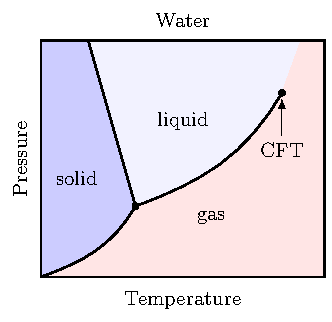
\includegraphics{Lectures/Figures/PT_diagram.pdf}
        \caption{Phase diagram of water. At the critical point, the system is described by a conformal field theory/CFT.}
        \label{fig:waterphase}
    \end{figure}
\end{itemize}

In this course we'll try to take a holistic perspective of QFT. The textbook is Srednicki - it's maybe not the best QFT textbook; it doesn't give good insights (come to lecture for that), but takes you through the details and developing techniques. Grade from weekly problem sets, assigned on Thursday and due the next Thursday.

\subsection{Review of Classical and Quantum Mechanics}
It will be useful to review the quantum simple harmonic oscillator as the simplest QFT is simply a collection of QSHOs.

\subsubsection*{Classical SHO - Variational Method}
Let's start with the classical SHO. Consider a (classical) point particle in a potential $V(x)$. 
\begin{figure}[htbp]
    \centering
    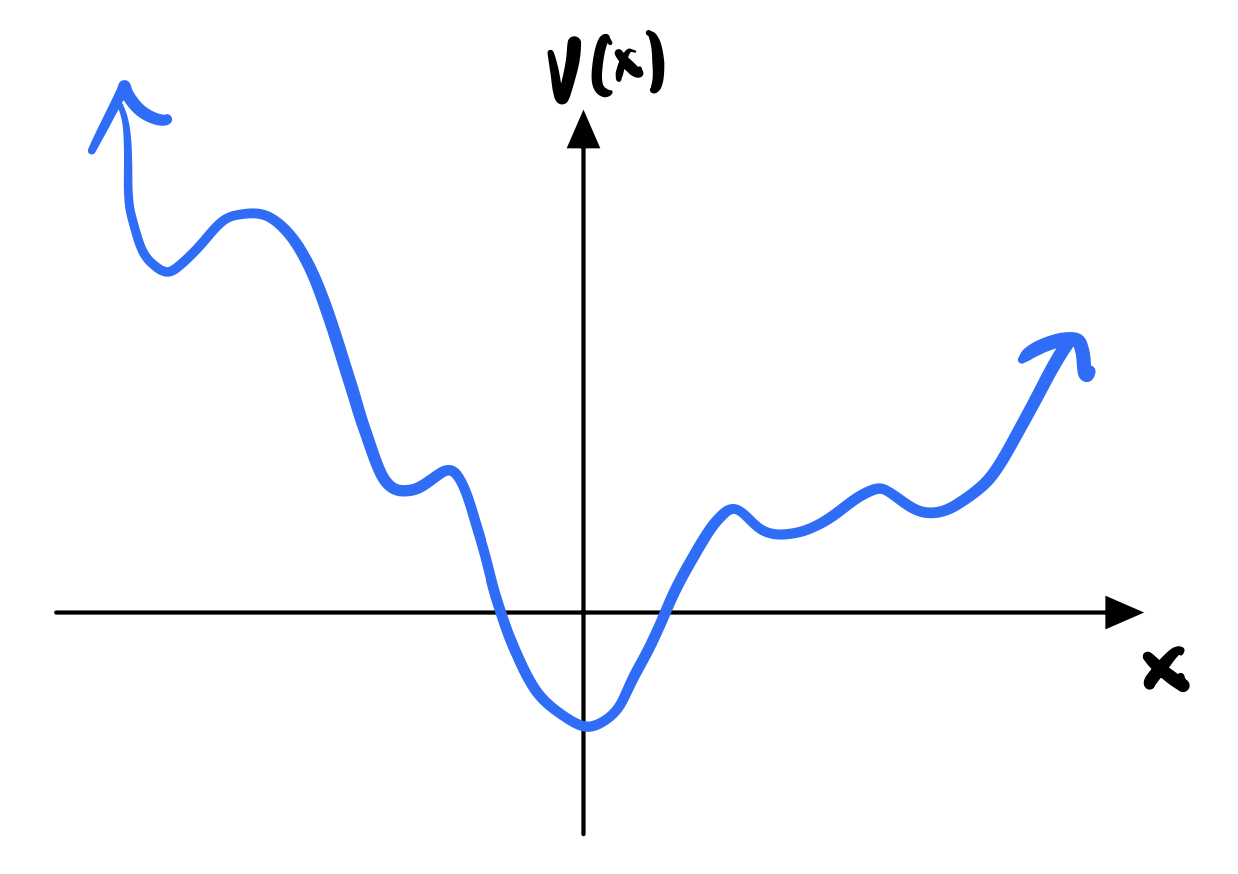
\includegraphics[scale=0.4]{Lectures/Figures/arbitrary_potential.png}
    \caption{Sketch of an arbitrary 1-D potential $V(x)$.}
    \label{fig:arbitrary_potential}
\end{figure}
Its dynamics is described by the action:
\begin{equation}
    S[x(t)] = \int dt \frac{1}{2}m\dot{x}(t) - V(x(t))
\end{equation}
where the first term is the kinetic energy and the second term is the potential energy.

To get the equation of motion from the action approach, we look for the trajectory $x(t)$ that extremizes the action (which is a \emph{functional}, as it depends on a function $x(t)$) $S[x(t)]$. We use a variational approach to find the extremizing trajectory. Under an arbitrary $\delta x(t)$ (to the true path $x(t)$), we must have $\delta S = 0$. Let us look at the variation, to linear order:
\begin{equation}
    0 = \delta S = \int dt m \dot{x}\dot{\delta x} - V'(x(t))\delta x
\end{equation}
Now, integrating by parts, we have:
\begin{equation}
    \int dt \dot{x}\dot{\delta x} = \left. \partial_t(\dot{x}\delta x) \right|_{-\infty}^\infty - \int dt \ddot{x}\delta x
\end{equation}
where the first term is a total derivative, which we take to be zero assuming the variation dies off at the infinite past and future. We then obtain:
\begin{equation}
    0 = \delta S = -\int dt \delta x(t)\left[m\ddot{x}(t) + V'(x(t))\right]
\end{equation}
Since this must vnaish for all variations $\delta x$, we obtain the equation of motion:
\begin{equation}
    \boxed{m\ddot{x}(t) + V'(x) = 0}.
\end{equation}

This is a nonlinear ODE, and difficult to solve; however when the potential is quadratic:
\begin{equation}
    V(x) = \frac{1}{2}kx^2
\end{equation}
\begin{figure}[htbp]
    \centering
    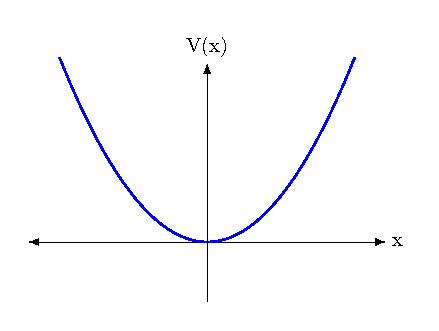
\includegraphics[]{Lectures/Figures/quad_potential.pdf}
    \caption{A quadratic potential $V(x) = \frac{1}{2}kx^2$.}
    \label{fig:quad_potential}
\end{figure}
it becomes linear and we can solve it! In this case, we have:
\begin{equation}
    0 = m\ddot{x} + kx
\end{equation}
The general solution is:
\begin{equation}
    x(t) = Ae^{i\omega_0t} + Be^{-i\omega_0t}
\end{equation}
where we have introduced the characteristic frequency $\omega_0 = \sqrt{k/m}$. $A, B$ are integration constants fixed by the initial conditions. Since we want $x(t) \in \RR$ for all $t$, this enforces $B = A^*$. 

\subsubsection*{Classical SHO - Hamiltonian Formalism}
We solve the same problem, but in the Hamiltonian formalism. We identify the conjugate momentum:
\begin{equation}
    p = \frac{\delta S}{\delta \dot{x}} = m\dot{x}
\end{equation}
And the Hamiltonian is given by:
\begin{equation}
    H = \dot{x}p - L = \frac{p^2}{m} - \frac{p^2}{2m} + V = \frac{p^2}{2m} + \frac{1}{2}kx^2
\end{equation}
and can be viewed as the generator of time translations. To obtain the EOM from the Hamiltonian, we consider the Poisson brackets:
\begin{subequations}
    \begin{align}
    \dot{x} &= \{x, H\}_{PB} \\
    \dot{p} &= \{p, H\}_{PB}
    \end{align}
\end{subequations}
Where $\{\}_{PB}$ denotes the Poisson bracket:
\begin{equation}
    \{f(x, p), g(x, p)\}_{PB} = \partial_x f \partial_p g - \partial_p f \partial_x g
\end{equation}
So the EOM become:
\begin{subequations}
    \begin{align}
        \dot{x} &= \partial_p H = \frac{p}{m} \\
        \dot{p} &= -\partial_x H = -kx
    \end{align}
\end{subequations}

From which we obtain:
\begin{equation}
    \dot{p} = m\ddot{x} = -kx
\end{equation}
which is precisely hte same equation we had previously.

A comment; the conjugate coordinate momentum pair satisfy:
\begin{equation}
    \{x, p\}_{PB} = 1.
\end{equation}

\subsection{The Quantum SHO}
In canonical quantization, one starts from the coordinates in phase space (in this case, $x$ and $p$) and then promotes them to quantum-mechanical operators satisfying canonical commutation relations:
\begin{equation}
    \{x, p\}_{PB} \to [\hat{x}, \hat{p}] = i\hbar
\end{equation}
where $\hbar$ is a constant with dimensions - by appropriate choice of units we can set it to 1, which we do for the remainder of this course. Thus, instead of measuring momentum in kg m/s, we will measure it in $\hbar$/m to make the commutator dimensionless.

$H$ is also now an operator; it has the same expression as before, but now involves $\hat{x}, \hat{p}$:
\begin{equation}
    \hat{H} = \frac{\hat{p}^2}{2m} + \frac{1}{2}k\hat{x}^2.
\end{equation}
$\hat{H}$ acts on states $\ket{\psi}$ of a Hilbert space. The dynamics are governed by the Schrodinger equation:
\begin{equation}
    i\partial_t \ket{\psi} = \hat{H}\ket{\psi}
\end{equation}
Acting on this equation with $\bra{x}$ a position eigenstate, we obtain the Scrodinger equation in position space:
\begin{equation}
    i\partial_t \psi(t, x) = -\frac{1}{2m}\partial_x^2\psi(t, x) + \frac{1}{2}kx^2\psi(t, x).
\end{equation}
where $\psi(t, x) \coloneqq \braket{x}{\psi}$ and we recall that $\hat{p} \to -i\partial_x$ when acting in position space (this can be derived from the canonical commutation relations).

This is a partial differential equation; in general, this is not trivial to solve (though we may of course put it on a computer and see the time evolution for arbitrary initial conditions). Instead of solving it fully generally, we look for stationary solutions:
\begin{equation}
    \psi(x, t) = e^{-iEt}\psi(x)
\end{equation}
We then obtain an ODE, which is slightly easier to work with:
\begin{equation}
    E\psi(x) = -\frac{1}{2m}\partial_x^2\psi(x) + \frac{1}{2}kx^2\psi(x).
\end{equation}
We would like for the solutions to be normalizable such that we are able to normalize $\psi(x)$ and interpret $\abs{\psi(x)}^2$ as a spatial probability distribution. Mathematically, this is the condition:
\begin{equation}
    \int dx \abs{\psi(x)}^2 < \infty.
\end{equation}
Although in the classical SHO we had an infinite, continuous set of solutions, the normalization condition interestingly reduces the set of solutions to a discrete (though still infinite) set. In this sense we have \emph{quantized} the SHO. We can label this discrete set of solutions as $\ket{n}$ for $n \in \NN$:
\begin{equation}
    \hat{H}\ket{n} = E_n\ket{n}.
\end{equation}

Let us review how to obtain the spectrum of the QSHO. We do this by diagonalizing $\hat{H}$, which we do via the method of raising and lowering operators, which are defined as linear combinations of $\hat{x}, \hat{p}$:
\begin{equation}
    \hat{a} = \frac{1}{\sqrt{2}}\left[\sqrt{m\omega_0}\hat{x} + i\frac{1}{\sqrt{m\omega_0}}\hat{p}\right]
\end{equation}
\begin{equation}
    \hat{a}^\dagger = \frac{1}{\sqrt{2}}\left[\sqrt{m\omega_0}\hat{x} - i\frac{1}{\sqrt{m\omega_0}}\hat{p}\right]
\end{equation}
The coefficients are chosen such that:
\begin{equation}
    [\hat{a}, \hat{a}^\dagger] = 1
\end{equation}
and such that:
\begin{equation}
    \hat{H} = \omega_0(\hat{a}^\dagger \hat{a} + \frac{1}{2})
\end{equation}
Defining $N \coloneqq \hat{a}^\dagger a$, the eigenstates are discrete; let $\ket{n}$ be the eigenstates of $\hat{N}$:
\begin{equation}
    \hat{N}\ket{n} = n\ket{n}.
\end{equation}
we show that $n \in \NN$. This follows as:
\begin{equation}\label{eq:lowering}
    \hat{N}\hat{a}\ket{n} = \hat{a}^\dagger \hat{a}\hat{a}\ket{n} = ([\hat{a}^\dagger, \hat{a}] - \hat{a}\hat{a}^\dagger)\hat{a}\ket{n} = -\hat{a}\ket{n} + \hat{a}\hat{a}^\dagger \hat{a}\ket{n} = (n-1)\hat{a}\ket{n}
\end{equation}
so $\hat{a}$ lowers the eigenvalue of $\hat{N}$ by one. In order for the spectrum to be bounded, we require a state annihilated by $\hat{a}$, i.e. that which $\hat{a}\ket{0} = 0$ (else there is no lower bound to the spectrum). We then note that:
\begin{equation}
    \hat{N}\ket{0} = \hat{a}^\dagger\hat{a}\ket{0} = 0 = 0\ket{0}
\end{equation}
thus this is an eigenstate (the ground state) of $\hat{H}$ with eigenvalue $\omega_0/2$. The rest of the spectrum can be built using $\hat{a}^\dagger$s. Via a similar argument to Eq. \eqref{eq:lowering}, it can be shown that $\hat{a}^\dagger$ increases the eigenvalue of $\hat{N}$ by one, and thus the eigenstates are:
\begin{equation}
    \ket{n} = \frac{(\hat{a}^\dagger)^n}{\sqrt{n!}}\ket{0}
\end{equation}
where $\braket{n}{n'} = \delta_{nn'}$, $\hat{N}\ket{n} = n\ket{n}$, and $\hat{H}\ket{n} = \omega_0(n + \frac{1}{2})\ket{n}$. Thus the spectrum is:
\begin{equation}
    \boxed{E_n = \omega_0(n + \frac{1}{2})}.
\end{equation}

This QSHO will be the building block from which we will construct quantum field theories.

\subsection{Free Scalar QFT}
Consider a SHO on every site of a $M$-site lattice:
\begin{figure}[htbp]
    \centering
    
\includegraphics[scale=0.4]{Lectures/Figures/qsho_chain.png}
    \caption{We begin to construct the simplest QFT, the free scalar QFT, by placing non-interacting quantum SHOs on sites of a lattice.}
    \label{fig:qsho_chain}
\end{figure}
The action is then simply the $M$-fold sum of our previous action
\begin{equation}
    S = m\sum_{j=1}^M\int dt \frac{1}{2}\dot{x}_j(t) - \frac{1}{2}\omega_0^2x_j(t) = \sum_{j=1}^M\int dt \frac{1}{2}\dot{\phi}_j^2(t) - \frac{1}{2}\omega_0^2\phi_j(t)
\end{equation}
where we have defined $\phi_j = \sqrt{m}x_j$. This is a quantum many-body system, but the solution to this is already known! It will simply be $M$ copies of the previous single-body system. Eigenstates are labelled by a collection of occupation numbers $\set{n_j}$, where:
\begin{equation}
    \ket{\set{n_j}} = \ket{n_1, n_2, \ldots, n_M}
\end{equation}
and the energy eigenvalues is just the sum of the individual energies:
\begin{equation}
    \hat{H}\ket{\set{n_j}} = \sum_j E_j \ket{\set{n_j}} = \sum_j \omega_0(n_j + \frac{1}{2})\ket{\set{n_j}}.
\end{equation}

\subsubsection*{Adding interactions}
This will become more interesting if we couple the SHOs, for example with nearest neighbour couplings. We add a term to the action:
\begin{equation}
    S = \sum_{j=1}^M \int dt \frac{1}{2}\dot{\phi_j}^2 - \frac{1}{2}\omega_0\phi_j^2 - \frac{1}{2}\frac{c^2}{\delta^2}(\phi_j - \phi_{j-1})^2
\end{equation}
The last term represents an energy penalty to the positions of neighbouring oscillators not being aligned. 

\begin{figure}[htbp]
    \centering
    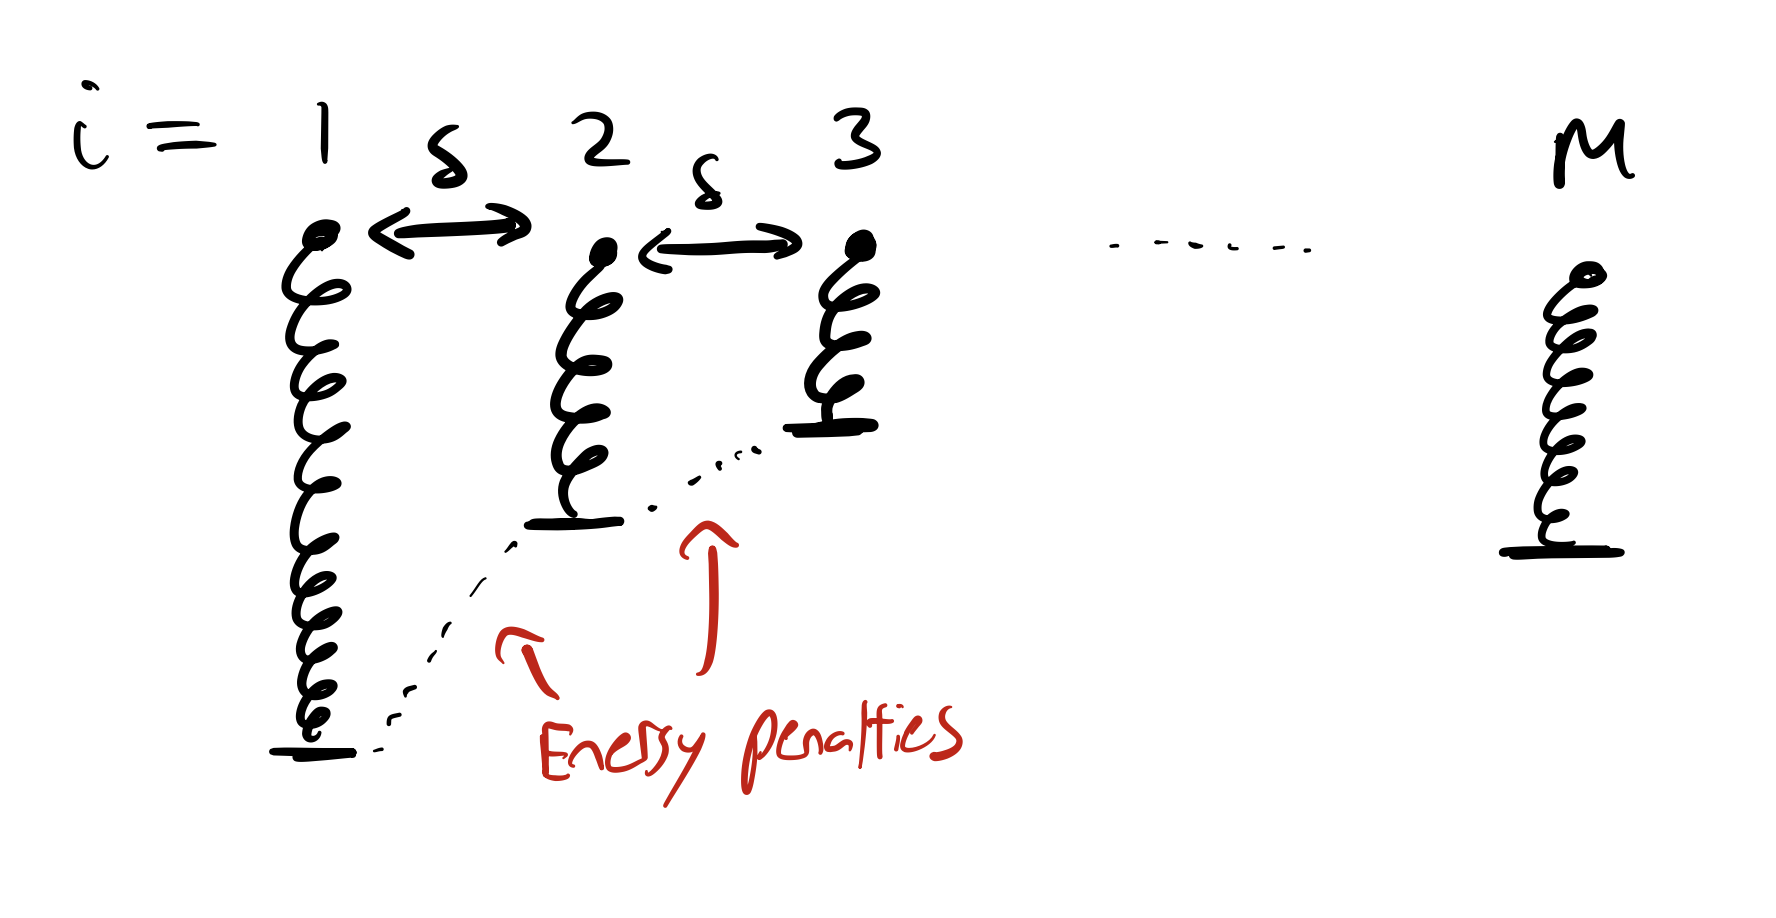
\includegraphics[scale=0.4]{Lectures/Figures/coupled_qsho_chain.png}
    \caption{We introduce couplings between QSHOs by imposing an energy penalty when neighbouring oscillators are misaligned. The relevant length scale of the interaction is given by the lattice spacing $\delta$.}
    \label{fig:coupled_qsho_chain}
\end{figure}

$\delta$ is the spacing between lattice sites and $c$ has the dimensions of velocity. The term must have units of $\frac{1}{t^2}$, and we see that $\frac{c^2}{\delta^2}$ indeed has this.

This turns out to be a much richer system! The action/Hamiltonian is not diagonal in the $i$ label. The trick is to do a change of basis, via a Fourier transform:
\begin{equation}
    \tilde{\phi}_k = \frac{1}{\sqrt{M}}\sum_{j=1}^Me^{-i\delta k j}\phi_j
\end{equation}
which we will show can be inverted:
\begin{equation}
    \phi_j = \frac{1}{\sqrt{M}}\sum_{k=1}^Me^{i\delta k j}\tilde{\phi}_k
\end{equation}
and $k \in \{-\frac{M}{2} + 1, \ldots, -1, 0, 1, \ldots, \frac{M}{2}\} \cdot \frac{2\pi}{L}$. We will then show that:
\begin{equation}
    S = \sum_k \int dt \frac{1}{2}\abs{\tilde{\phi}_k}^2 - \frac{1}{2}\omega_0^2\abs{\tilde{\phi}_k}^2 - \frac{c^2}{\delta^2}(1 - \cos(k\delta))\abs{\tilde{\phi}_k}^2.
\end{equation}
We then notice that the $\tilde{\phi}_k$s don't talk to each other/are decoupled! We are back to having decoupled SQHOs, just in a different basis. This immediately gives the spectrum.
\newpage
\section{Free Scalar Field Theory Part 2, Lorentz Invariance}
Recall the action for a collection of QSHOs coupled with nearest neighbour interactions:
\begin{equation}
    S = \sum_{j=1}^M \int dt \frac{1}{2}\dot{\phi}_j^2 - \frac{1}{2}\omega_0^2\phi_j - \frac{1}{2}\frac{c^2}{\delta^2}\left(\phi_j - \phi_{j+1}\right)^2
\end{equation}
where we have periodic boundary conditions, such that $\phi_{j+M} = \phi_j$. The lattice spacing is $\delta$ such that the total length of the chain is $L = M\delta$.

We will solve this via a change of basis of degrees of freedom $\phi_i$ to momentum space:
\begin{equation}
    \tilde{\phi}_k = \frac{1}{\sqrt{M}}\sum_{j=1}^M e^{-ik\delta j}\phi_j, \quad k \in \set{-\frac{M}{2} + 1, \ldots, -1, 0, 1, \ldots, \frac{M}{2}} \cdot \frac{2\pi}{L}
\end{equation}
Note that the $\tilde{\phi}_k$s are no longer real, but they do satisfy the reality condition:
\begin{equation}
    (\tilde{\phi}_k)^* = \tilde{\phi}_{-k}
\end{equation}

We will show:
\begin{equation}\label{eq:actionmomentumspace}
    S = \sum_k \int dt \frac{1}{2}\abs{\dot{\tilde{\phi}}_k}^2 - \frac{1}{2}\omega_0^2\abs{\tilde{\phi}_k}^2 - \frac{c^2}{\delta^2}(1 - \cos(\delta k))\abs{\tilde{\phi}_k}^2
\end{equation}
The Fourier transform diagonalizes the action (each of the $\tilde{\phi}_k$s are independent) and we can also now see that the characteristic frequency of the $\tilde{\phi}_k$ has a dependence on $k$ through the $\cos(\delta k)$. 

Note that the inverse Fourier transform is given by:
\begin{equation}
    \phi_j = \frac{1}{\sqrt{M}}\sum_k e^{ik\delta j}\tilde{\phi}_k
\end{equation}
To check that this is the case, let us plug in the expression for the forwards Fourier transform and check that we recover $\phi_j$:
\begin{equation}
    \phi_j = \frac{1}{M}\sum_k \sum_{j'}e^{ik\delta j}e^{-ik\delta j'}\phi_{j'} = \frac{1}{M}\sum_{j'}\phi_{j'}\sum_k e^{ik\delta(j - j')} = \frac{M}{M}\sum_{j'}\phi_{j'}\delta_{jj'} = \phi_j
\end{equation}
In the second equality we commute the two sums and first carry out the sum over $j'$. For the third equality (where we carry out the sum over $j'$) note that if $j = j'$ then the argument of the exponential is zero and so the sum is just an $M$-fold sum of 1, i.e. just gives $M$. If $j - j' = 1$, then the sum is $\sum_k e^{ik\delta}$. The first term in the sum is $e^{i(0)} = 1$, the next term is $e^{i\frac{2\pi}{L}\delta} = e^{\frac{2\pi}{M}}$, the next is $ee^{\frac{2\pi}{M}\cdot 2}$, and so on. This is a sum over points on the unit circle in $\mathbb{C}$ for which the sum is just the center of mass, i.e. 0. 

\begin{figure}[htbp]
    \centering
    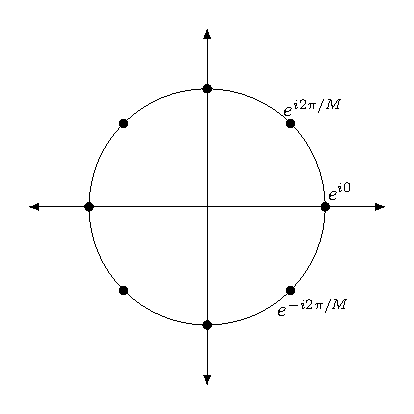
\includegraphics[]{Lectures/Figures/unit_circle_sum.pdf}
    \caption{When looking at $\sum_k e^{ik\delta(j - j')}$, for $k \in \set{-\frac{M}{2} + 1, \ldots, -1, 0, 1, \ldots, \frac{M}{2}} \cdot \frac{2\pi}{L}$, and $\abs{j-j'}=1$, we can view the sum as going over points in the complex unit circle. Above, we have $M = 8$. The sum of the points has its center of mass in the center of the unit circle, i.e. $0$ and so the sum evaluates to zero. For $\abs{j - j'} > 1$, we simply skip points (the sum goes around the circle at ``higher frequency''), but the sum cancells in the same way.}
    \label{fig:unit_circle_sum}
\end{figure}

For $j - j' \neq 0$ in general, we repeat the argument (potentially skipping point as larger $j-j'$ has larger frequency around the circle). This is why we conclude that $\sum_{k}e^{ik\delta(j-j')} = M\delta_{jj'}$.

Let's now convert the action:
\begin{equation}
    \sum_{j=1}^M \phi_j^2 = \frac{1}{M}\sum_j\left(\sum_{j}e^{ik\delta j}\tilde{\phi}_k\right)\left(\sum_{k'}e^{ik'\delta j}\tilde{\phi}_{j'}\right) = \frac{1}{M}\sum_{kk'}\tilde{\phi}_k\tilde{\phi}_{k'}\sum_j e^{ik\delta j}e^{ik'\delta j} = \frac{1}{M}\sum_{kk'}\tilde{\phi}_k\tilde{\phi}_{k'} \sum_{j=1}^M e^{i\delta j (k + k')}
\end{equation}

Applying the same argument as we saw in checking the inverse Fourier transform, we know that $\sum_{j=1}^M e^{i\delta j (k + k')} = M\delta_{k', -k}$ so:
\begin{equation}
    \sum_{j=1}^M \phi_j^2 = \sum_{kk'}\tilde{\phi}_k\tilde{\phi}_{k'}\delta_{k',-k} = \sum_k \tilde{\phi}_k\tilde{\phi}_{-k} = \sum_{k}\abs{\tilde{\phi}_k}^2
\end{equation}
where in the last equality we use the reality condition $(\tilde{\phi}_k)^* = \tilde{\phi}_{-k}$.

The time derivative term works out exactly the same way, just take the dot along for the ride:
\begin{equation}
    \sum_{j=1}^M \dot{\phi_j}^2 = \sum_{k}\abs{\dot{\tilde{\phi}}_k}^2.
\end{equation}

The term that is more subtle (and more interesting) is the interaction term. Let us study this now.

\begin{equation}
    \sum_{j=1}^M (\phi_j - \phi_{j+1})^2 = \frac{1}{M}\sum_j \left(\sum_k \left(e^{ik\delta j}\tilde{\phi}_k - \sum_k e^{ik\delta(j+1)}\tilde{\phi}_{k}\right)\right)^2
\end{equation}
The two terms appearing are almost identical, so we factor out the piece that looks the same:
\begin{equation}
    \sum_{j=1}^M (\phi_j - \phi_{j+1})^2 = \frac{1}{M}\sum_j \left(\sum_k \tilde{\phi}_k e^{ik\delta j}\left(1 - e^{ik\delta}\right)\right)\left(\sum_{k'}\tilde{\phi}_{k'}e^{ik'\delta k}(1 - e^{ik'\delta})\right)
\end{equation}
Now doing the trick we've seen twice already, we interchange the order of the summations and take the $j$ sum first:
\begin{equation}
    \sum_{j=1}^M (\phi_j - \phi_{j+1})^2 = \frac{1}{M}\sum_{kk'}\tilde{\phi}_k \tilde{\phi}_{k'}(1 - e^{ik\delta})(1-e^{ik'\delta})\sum_j e^{i\delta j(k+k')} = \frac{1}{M}\sum_{kk'}\tilde{\phi}_k \tilde{\phi}_{k'}(1 - e^{ik\delta})(1-e^{ik'\delta}) M\delta_{k',-k}
\end{equation}
We are then left with:
\begin{equation}
    \sum_{j=1}^M (\phi_j - \phi_{j+1})^2 = \sum_{k}\tilde{\phi}_k\tilde{\phi}_{-k}(1 - e^{ik\delta})(1-e^{-ik\delta}) = \sum_{k}\abs{\tilde{\phi}_k}^2 (2 - (e^{ik\delta} + e^{-ik\delta})) = 2\sum_k \abs{\tilde{\phi}_k}^2(1-\cos(k \delta))
\end{equation}
where the last equality follows via Euler's formula. We have thus successfully obtained the action $S$ in the $k$-basis. The modes are now not labelled by sites, but by the wavevector (number as we are in 1-D) $k$. 

Question: How could we have guessed that this was a good choice of basis? One intuition is that the action (in the position basis) was translation invariant. When we have a translation invariant problem, momentum is conserved and thus the momentum basis is convenient to work in.

Since we now have diagonalized the action - we have $M$ decoupled QSHOs labelled by $k$; the eigenstates and spectrum easily follow. The eigenstates are:
\begin{equation}
    \ket{\set{n_k}} = \ket{n_{(-\frac{M}{2} + 1)\frac{2\pi}{L}}, \ldots, n_{-\frac{2\pi}{L}}, n_0, n_{\frac{2\pi}{L}}, \ldots, n_{\frac{M}{2}\frac{2\pi}{L}}}
\end{equation}
The energy is simply the sum of the energy of each of the modes:
\begin{equation}
    \hat{H}\ket{\set{n_k}} = E_{\set{n_k}}\ket{\set{n_k}} = \sum_k E_{n_k}\ket{\set{n_k}}
\end{equation}
where:
\begin{equation}
    E_{n_k} = (n_k + \frac{1}{2})\sqrt{\omega_0^2 + 2\frac{c^2}{\delta^2}(1-\cos(\delta k))}
\end{equation}
which is obtained by looking at the action in Eq. \eqref{eq:actionmomentumspace}, and taking the square root of the terms multiplying $\frac{1}{2}\abs{\tilde{\phi}_k}^2$. 

We have thus solved our first nontrivial quantum many-body problem! Although simply, this already has applications in nature; this simple model describes phonons in a crystal, and can be used to predict the heat capacity of a crystal. Note that in a crystal, the spacing $\delta$ is finite (the lattice/atomic spacing). However, what we will do now is take the continuum limit.

\subsection{Continuum Limit: QM to QFT}
What we really did above is solve a quantum-mechanics problem; we now take $\delta \to 0$ and go from QM to QFT. Let's see what happens to the $\frac{c^2}{\delta^2}(1-\cos(\delta k))$ term in this limit. Taylor expanding the cosine, we have:
\begin{equation}
    \lim_{\delta \to 0 }\frac{c^2}{\delta^2}(1 - \cos(\delta k)) = \lim_{\delta \to 0}\frac{c^2}{\delta^2}\left(1 - \left(1 - \frac{(\delta k)^2}{2}\right)\right) = \frac{1}{2}c^2k^2
\end{equation}
Thus the action becomes:
\begin{equation}
    S = \sum_k \int dt \frac{1}{2}\abs{\dot{\tilde{\phi}}_k^2} - \frac{1}{2}(\omega_0^2 + c^2k^2)\abs{\tilde{\phi}_k}^2
\end{equation}
and the spectrum becomes:
\begin{equation}
    E_{n_k} = (n_k + \frac{1}{2})\sqrt{\omega_0^2 + c^2k^2}
\end{equation}
You will explore this a little more in the first problem set.

Let us see what happens in position space in the continuum limit! Recall the action in position space:
\begin{equation}
    S = \sum_{j=1}^M \int dt \frac{1}{2}\dot{\phi}_j^2 - \frac{1}{2}\omega_0^2\phi_j - \frac{1}{2}\frac{c^2}{\delta^2}\left(\phi_j - \phi_{j+1}\right)^2
\end{equation}
Then noting that, $\phi_j = \phi(x = j\delta)$ in the continuum limit the interaction term becomes:
\begin{equation}
    \lim_{\delta \to 0} \left(\frac{\phi(j\delta + \delta) - \phi(j\delta)}{\delta}\right)^2 = (\partial_{x=\delta j} \phi)^2
\end{equation}
where we recognize the definition of the derivative. In addition, the sum over lattice sites becomes an integral over position space, so the action becomes:
\begin{equation}
    S = \int dt \int dx \frac{1}{2}(\partial_t \phi(t, x))^2 - \frac{1}{2}c^2(\partial_x \phi(t, x))^2 - \frac{1}{2}\omega_0^2(\phi(t, x))^2
\end{equation}
where we can (loosely) recognize the wavevector $k$ becoming $\partial_x$ in position space. Now, let's obtain the classical equation of motion for this system:
\begin{equation}
    0 = \delta S = \int dtdx \dot{\phi}\dot{\delta \phi} - c^2 \partial_x \phi \partial_x \delta \phi - \omega_0^2 \phi \delta \phi
\end{equation}
Like last time, we wish to factor out $\delta \phi$, as we can then conclude that whatever it multiples must be zero. We integrate by parts, and we choose the variation to be zero at spatial/temporal infinity so that we may throw away the boundary term (we don't \emph{have} to impose this - not doing so would give us an extra condition, but for now we don't care about the boundaries). We are left with:
\begin{equation}
    0 = \int dt dx \delta \phi(-\partial_t^2\phi + c^2\partial_x^2 \phi - \omega_0^2 \phi)
\end{equation}
and since this must be true for all choices of variations $\delta \phi(t, x)$, we obtain:
\begin{equation}
    \boxed{(\partial_t^2 - c^2\partial_x^2 + \omega_0^2)\phi(t, x) = 0}
\end{equation}
which is the classical equation of motion for this field, known as the \emph{Klein-Gordon equation}. The first two terms we recognize as those appearing in the standard wave equation, with solutions $f(x \pm ct)$. The $\omega_0^2$ is an addition to the wave equation, which tells us that disturbances propagate at speed $< c$. Although the dynamics are a little more complex than the wave equation, it is still a linear PDE and can be solved.

This equation is accidentally relativistic (it is Lorentz covariant, as we shall soon see), without trying. Interestingly, $c$ may not be the speed of light in materials, yet such systems have a sort of Lorentz symmetry.

Note that even with interactions, this QFT is still called free scalar field theory, as the action is quadratic in the field. We will also in the future look at (non-linear) interactions, which will be more difficult and lead to further phenomenology.

\subsection{Lorentz Invariance}
Some systems have relativistic symmetry, in which case we should use it; it is also just a great example of how we can use symmetries to constrain and understand QFTs. Finally, it is a symmetry of nature, so we should care about it, as humans, not just as physicists\footnote{Luca: I try to tell this to my friends, but it doesn't really work...}. Symmetries are described by groups, and then we can do things like classifying particles by representations of groups (e.g. spin-1/2 particles described by representations of the Lorentz group).

Historically, Maxwell's equations were the first hint that the laws of nature are \emph{not} invariant under Galilean boosts:
\begin{equation}
    \v{x} \to \v{x} + \delta\v{v}t, \quad t \to t
\end{equation}
(where time is left invariant) but rather invariant under Lorentz boosts:
\begin{equation}\label{eq:infinitesimalLorentz}
    \v{x} \to \v{x} + \delta\v{v}t, \quad t \to t + \frac{\delta\v{v} \cdot \v{x}}{c^2}
\end{equation}
where we note that time is also transformed. At low velocities $\abs{\v{v}} \ll c$ this effect is small so we may be able to neglect it, but (e.g.) in electromagnetism or in relativistic systems it becomes highly relevant.

From now on, we choose units such that $c = 1$. 

Note that the transformations appearing in Eq. \eqref{eq:infinitesimalLorentz} are the infinitesimal form, but this is all we really need; from these we can easily find the finite versions.

How can we understand Lorentz transformations? They are those that leave \emph{spacetime} distance between pairs invariant:
\begin{equation}
    \abs{\v{x}}^2 - t^2 \to (\v{x} + \delta\v{v}t)^2 - (t + \delta\v{v} \cdot \v{x})^2 = \abs{\v{x}}^2 - t^2 + 2\v{x} \cdot \delta \v{v}t - 2t\v{x}\cdot \delta \v{v} = \abs{\v{x}}^2 - t^2
\end{equation}
where we neglect terms $O((\delta \v{v})^2)$. 

\begin{figure}[htbp]
    \centering
    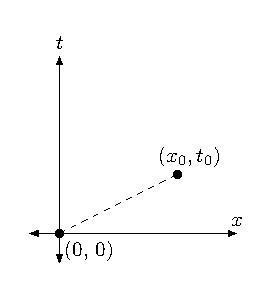
\includegraphics[]{Lectures/Figures/spacetime_interval.pdf}
    \caption{Lorenz transformations leave the \emph{spacetime} distance $\abs{\v{x}}^2 - t^2$ between two spacetime points invariant, here $x_0^2 - t_0^2$.}
    \label{eq:spacetime_interval}
\end{figure}

We here consider a more compact notation in the form of 4-vectors, where we group the 3 spatial and 1 temporal (3+1) coordinates into a single vector:
\begin{equation}
    x^\mu = (t, x^1, x^2, x^3)
\end{equation}
where we can then write the spacetime distance as:
\begin{equation}
    -t^2 + \v{x}^2 = \m{t \\ x_1 \\ x_2 \\ x_3}^T \m{-1 & 0 & 0 & 0 \\ 0 & 1 & 0 & 0 \\ 0 & 0 & 1 & 0 \\ 0 & 0 & 0 & 1}\m{t \\ x_1 \\ x_2 \\ x_3}
\end{equation}
the $4 \times 4$ matrix appearing above is the Minkowski metric $\eta_{\mu\nu} = \text{diag}(-1, 1, 1, 1)$, and we can write the spacetime interval as:
\begin{equation}
    -t^2 + \abs{\v{x}}^2 = x^\mu \eta_{\mu \nu} x^\nu = x^2
\end{equation}
where $\mu, \nu = 0, 1, \ldots, d$ where $x^0 = t$ and $d$ is the spatial dimension, $3$ in this case. This is the correct choice of the metric signature, according to Luca, though it was met with murmurs of mild controversy from the crowd.

\subsection{Classifying all Lorentz Transformations}
Let us try to find \emph{all} Lorentz transformations, i.e. linear transformations:
\begin{equation}
    x^\mu \to \Lambda^{\mu}_\nu x^\nu = x^{,\mu}
\end{equation}
that leave the spacetime interval invariant:
\begin{equation}
    x^2 \equiv x^\mu \eta_{\mu\nu} x^\nu \to \eta_{\mu\nu}x^{'\mu}x^{'\nu} = \eta_{\mu\nu}\Lambda^\mu_\alpha \Lambda^\nu_\beta x^\alpha x^\beta
\end{equation}
This yields the condition:
\begin{equation}
    \eta_{\mu\nu} \Lambda^\mu_\alpha \Lambda^\nu_\beta = \eta_{\alpha\beta}
\end{equation}
i.e. the $\Lambda$ matrices leave the Minkowski metric invariant.

Notice that these include spatial rotations, which rotates space and leaves time invariant! These satisfy $t \to t$ and $\abs{\v{x}}^2 \to \abs{\v{x}}^2$ (rotations leave spatial distances invariant). So, one subclass of Lorentz transformations are
\begin{equation}
    \Lambda = \m{1 & 0 & 0 & 0 \\ 0 & & & \\ 0 & & R & \\ 0 & & &}
\end{equation}
Where $R$ are the $3 \times 3$ rotation matrices satisfying$R^T \cdot R = \II$.

Note that Lorentz transformations form a group; let us check that they satisfy the group axioms. (1) If $\Lambda_1, \Lambda_2 \in G$, then:
\begin{equation}
    (\Lambda_1 \Lambda_2)^T \eta (\Lambda_1 \Lambda_2) = \Lambda_2^T (\Lambda_1^T \eta \Lambda_1) \Lambda_2 = \Lambda_2^T \eta \Lambda_2 = \eta
\end{equation}
so $\Lambda_1\Lambda_2 \in G$. (2) The $\Lambda$s are just matrices, so clearly their multiplication is associative:
\begin{equation}
    \Lambda_1(\Lambda_2\Lambda_3) = (\Lambda_1\Lambda_2)\Lambda_3.
\end{equation}
(3) There exists the identity element $\mathbb{I}$; this is just $\Lambda = \text{diag}(1, 1, 1, 1)$ which maps $x^\mu \to x^\mu$. Finally (4) There exists an inverse $\Lambda^{-1} \in G$ such that $\Lambda^{-1}\Lambda = \mathbb{I}$. Intuitively this is true, e.g. for rotations we just rotate in the opposite direction and that is the inverse transformation. We will examine the condition more closely next class. 

\newpage
\section{Lorentz Invariance Part 2, Transforming Fields}

\subsection{Inverses of Lorentz Transformations}
Recall the Lorentz transformations:
\begin{equation}
    X^\mu \to X'^\mu  = \Lambda^\mu_\nu X^\nu
\end{equation}
Which has the property of preserving spacetime distance:
\begin{equation}
    (X')^2 = X^2 = X^\mu X^\nu \eta_{\mu\nu}.
\end{equation}
Where $\eta = \text{diag}(-1, 1, 1, 1)$ is the Minkowski metric and $x^\mu = (x^0 = t, x^1, x^2, x^3)$. Thus they have the property:
\begin{equation}
    \eta_{\mu\nu}\Lambda^\mu_\alpha \Lambda^\nu_\beta = \eta_{\alpha\beta}
\end{equation}
or alternatively:
\begin{equation}
    \Lambda^T \eta \Lambda = \eta
\end{equation}

The Lorentz transformations form a group $O(1, 3)$, where $O$ stands for orthogonal. Last time we discussed the group axioms, one of which is that each group element has an inverse. Thus to conclude our argument about Lorentz transformations forming a group, for a given $\Lambda \in O(1, 3)$ let's find its inverse. To this end, we notice:

\begin{equation}
    \eta \Lambda^T \eta \Lambda = \eta(\eta) = \II
\end{equation}
thus:
\begin{equation}
    \Lambda^-1 = \eta \Lambda^T \eta.
\end{equation}
The inverse condition can also be phrased as:
\begin{equation}
    (\Lambda^{-1})^\mu_{\phantom{i}\nu} \Lambda^\nu_{\phantom{i}\lambda} = \delta^\mu_\lambda
\end{equation}
So the matrix elements are:
\begin{equation}
    (\Lambda^{-1})^\mu_{\phantom{i}\nu} = \eta^{\mu\alpha}\Lambda_{\phantom{i}\alpha}^\beta \eta_{\beta\nu}
\end{equation}

For more compact notation, it is often convenient to raise and lower indices using the Minkowski metric. For example:
\begin{equation}
    x_\mu = \eta_{\mu\nu}x^\nu.
\end{equation}
But be careful! Note that this means:
\begin{equation}
    x_\mu = (-t, x^1, x^2, x^3) \neq x^\mu.
\end{equation}
With this convention, we can write:
\begin{equation}
    (\Lambda^{-1})^{\mu}_{\phantom{i}\nu} = \Lambda_\nu^{\phantom{i}\mu}
\end{equation}
Note that Greek indices $\alpha, \beta, \mu, \nu$ we take to run from $0, \ldots, 3$ and regular letters $i, j, k, l$ we take to run from $1, \ldots, 3$ (spatial only).

\subsection{Infinitesimal Lorentz Transformations}
We consider infinitesimal versions of the Lorentz transformations; this makes the analysis more simple, and we can build up the finite versions from the infinitesimal ones. Thus, we consider:
\begin{equation}
    \Lambda = \II + \delta \omega
\end{equation}
thus:
\begin{equation}
    \Lambda^\mu_{\sp\nu} = \delta_\nu^\mu + \delta\omega^\mu_{\sp\nu}
\end{equation}
Thus for $\Lambda \in O(1, 3)$:
\begin{equation}
    \eta = \Lambda^T \eta \Lambda = (\II + \delta\omega^T)\eta(\II + \delta\omega) \approx \eta + \eta\delta\omega + \delta\omega^T \eta
\end{equation}
Thus:
\begin{equation}
    0 = (\eta\delta\omega)_{\mu\nu} + (\delta\omega^T\eta)_{\mu\nu} = \eta_{\mu\alpha}\delta\omega^\alpha_{\sp\nu} + \delta^\alpha_{\sp\mu}\eta_{\alpha\nu}.
\end{equation}
Let us define:
\begin{equation}
    \delta\omega_{\alpha\beta} = \eta_{\alpha\mu}\delta\omega^\mu_{\sp\beta}
\end{equation}
So then:
\begin{equation}
    0 = \delta\omega_{\mu\nu} + \delta\omega_{\nu\mu} \implies \delta\omega_{\mu\nu} = -\delta\omega_{\nu\mu} 
\end{equation}
i.e. the $\delta\omega$ matrix is antisymmetric! This might remind you of rotations; where the generators are antisymmetric. This tells us the general structure of infinitesimal Lorentz transformations; they are parametrized by antisymmetric matrices. Thus, the question of classifying Lorentz transformations becomes how many antisymmetric matrices they are.

In $D = 2$, we have a single independent antisymmetric matrix (0s on the diagonal, $a$ on the off diagonal, and $-a$ on the other off diagonal), corresponding to a boost. In general for $D$ dimensions we have $\frac{D(D-1)}{2}$ independent antisymmetric matrices; this can be seen from the fact that the diagonals are always zero, and then the upper triangle of the matrix - of which there are $\frac{D(D-1)}{2}$ entries - specifies the matrix (the lower triangle is fixed by antisymmetry). In $D = 4$, this corresponds to 6 independent infinitesimal Lorentz transformations; 3 rotations and 3 boosts. In a flat world (i.e. $D = 3$) we have 3, corresponding to 1 rotation and 2 boosts.

\subsection{Action of Symmetries - Representations}
In a little while, we will consider QFTs that have these symmetries. We are thus interested in learning how these symmetries act on the states. In QM and QFT, symmetries act as unitary operators on the Hilbert space.

For example, for a given Lorentz transformation $\Lambda$, there is a unitary operator $U(\Lambda)$ which acts on the Hilbert space, i.e.
\begin{equation}
    \ket{\psi} \to U(\Lambda)\ket{\psi}.
\end{equation}
where $U(\Lambda)^\dagger = U(\Lambda)^{-1}$. Alternatively, we can consider their action on operators:
\begin{equation}
    O \to U(\Lambda)^\dagger O U(\Lambda)
\end{equation}
This is a representation of the group symmetry, and this representation must be faithful. In particular:
\begin{equation}
    U(\Lambda_1)U(\Lambda_2) = U(\Lambda_1\Lambda_2)
\end{equation}
which implies:
\begin{equation}
    U(\II_G) = \II
\end{equation}
as well as:
\begin{equation}
    U(\Lambda)U(\Lambda^{-1}) = U(\II_G) = \II \implies U(\Lambda^{-1}) = U(\Lambda)^\dagger
\end{equation}
note that the $\II_G$ appearing in $(\cdot)$ is the identity group element, while the $\II$ appearing on the RHS is the identity operator. We drop the subscript as which is a group element/operator should be clear from context.

% A general note; representations are a mathematical concept which are different ways a group can act. For example on coordinates, we have the vector representation $x^\mu \to \Lambda^{\mu}_\nu x^\nu$, the trivial representation $x^2 \to ... = x^2$, or the tensor representation $x^\mu x^\nu = \Lambda^\mu_\alpha \Lambda^\nu_\beta x^\alpha x^\beta$.

For this course, we will generally consider faithful representations, though there are some cases where this is broken in a small way, e.g. up to a phase where $U(\Lambda_1)U(\Lambda_2) = U(\Lambda_1\Lambda_2)e^{i\alpha_{12}}$. 

So, if we consider the unitary representation of the infinitesimal Lorentz transformations:
\begin{equation}
    U(\II + \delta\omega) = \II + \frac{i}{2}\delta\omega_{\mu\nu}\hat{M}^{\mu\nu}
\end{equation}
here, $\hat{M}$ is a Hermitian operator:
\begin{equation}
    (\hat{M}^{\mu\nu})^\dagger = \hat{M}^{\mu\nu}.
\end{equation}
In a QFT, we will make $\hat{M}$ out of $\hat{a}_k, \hat{a}_k^\dagger, \hat{\phi}$ etc. We can think of $\hat{M}$ as a matrix of operators, acting (here) on an infinite-dimensional Hilbert space.

An observation; Lorentz transformations act on coordinates in a continuous way; so the only way to accommodate this is to have fields, which are infinite-dimensional.

We now derive very general results about QFTs with Lorentz invariance. We consider:
\begin{equation}\label{eq:transformedLorentztransform}
    U(\Lambda)^{-1}U(\II + \delta \omega)U(\Lambda) = U(\Lambda^{-1}(\II + \delta\omega)\Lambda) = U(\II + \Lambda^{-1}\delta\omega\Lambda) = \II + \frac{i}{2}\delta\omega'_{\alpha\beta}\hat{M}^{\alpha\beta}
\end{equation}
Where we have notated $\delta\omega' = \Lambda^{-1}\delta\omega\Lambda$. Writing out its components:
\begin{equation}
    \delta\omega'^{\alpha}_{\sp\beta} = (\Lambda^{-1})^\alpha_{\sp\mu} \delta\omega^\mu_{\sp\nu}\Lambda^\mu_{\sp\beta} = \Lambda^{\sp\alpha}_{\mu}\delta\omega^\mu_{\sp\nu}\Lambda^\nu_{\sp\beta}
\end{equation}
Thus:
\begin{equation}
    \delta\omega'_{\alpha\beta} = \Lambda^\mu_{\sp\alpha}\Lambda^\nu_{\sp\beta}\delta\omega_{\mu\nu}
\end{equation}
On the other hand, if we work out the LHS of Eq. \eqref{eq:transformedLorentztransform}, we have:
\begin{equation}
    U(\Lambda)^{-1}\left(1 + \frac{i}{2}\delta\omega_{\mu\nu}\hat{M}^{\mu\nu}\right)U(\Lambda).
\end{equation}
Thus comparing the left and right hand sides:
\begin{equation}\label{eq:LorentzonLorentz}
    U(\Lambda)^{-1}\hat{M}^{\mu\nu}U(\Lambda) = \Lambda^\mu_{\sp\alpha}\Lambda^\nu_{\sp\mu}\hat{M}^{\alpha\beta}
\end{equation}
Thus we see that we have a collection/multiplet of six operators $\hat{M}^{\mu\nu}$ (the generators of the Lorentz group) that get shuffled by Lorentz transformations. Thus, we can say that the generators $\hat{M}^{\mu\nu}$ transform in a \emph{tensor representation} of the Lorentz group.

\subsection{The Lorentz Algebra}
So, we have started to understand how Lorentz symmetries act on themselves. The statements that follow from symmetry are very simple and universal (in contrast to a lot of things about QFT)... Let's push this a little bit more to get one more interesting property. Let's also take the symmetry $\Lambda$ to be infinitesimal:
\begin{equation}
    \Lambda = \II + \delta\omega
\end{equation}
thus learning how infinitesimal Lorentz transformations act on each other. Taking $\Lambda$ to be infinitesimal in Eq. \eqref{eq:LorentzonLorentz}, we have (to leading order) on the LHS:
\begin{equation}
    \left(\II - \frac{i}{2}\delta\omega_{\alpha\beta}\hat{M}^{\alpha\beta}\right)\hat{M^{\mu\nu}}\left(\II + \frac{i}{2}\delta\omega_{\alpha\beta}\hat{M}^{\alpha\beta}\right) \approx \hat{M}^{\mu\nu} - \frac{i}{2}\delta\omega_{\alpha\beta}[\hat{M}^{\alpha\beta}, \hat{M}^{\mu\nu}]
\end{equation}
where we note that the inverse of the infinitesimal transformation simply flips the sign of $i$. The RHS of Eq. \eqref{eq:LorentzonLorentz} gives:
\begin{equation}
    \left(\delta^\mu_\alpha + \delta\omega^\mu_{\sp\alpha}\right)\left(\delta^\nu_\beta + \delta\omega^\nu_{\sp\beta}\right)\hat{M}^{\alpha\beta} \approx \hat{M}^{\mu\nu} + \delta\omega^\mu_{\sp\alpha}\hat{M}^{\alpha\nu} + \delta\omega^{\nu}_{\sp\beta}\hat{M}^{\mu\beta} = \hat{M}^{\mu\nu} + \delta\omega_{\alpha\beta}\left(\eta^{\alpha\nu}\hat{M}^{\mu\beta} - \eta^{\mu\beta}\hat{M}^{\alpha\nu}\right)
\end{equation}
where we note the swap of indices causes the flip of the sign in the last $\hat{M}$ term due to antisymmetry.

We want to now equate the two pieces; however note a small subtlety! $\delta\omega_{\alpha\beta}$ is \emph{not} a fully general matrix; it is a general \emph{antisymmetric} matrix, and thus places no constraint on the symmetric part of what it multiplies. So, we need to put the RHS expression into antisymmetric form via antisymmetrization:
\begin{equation}\label{eq:Lorentzalgebra}
    \boxed{[\hat{M}^{\alpha\beta}, \hat{M}^{\mu\nu}] = i\left(\eta^{\alpha\nu}\hat{M}^{\mu\beta} - \eta^{\mu\beta}\hat{M}^{\alpha\nu} - (\alpha \leftrightarrow \beta)\right)}
\end{equation}
where we note that the antisymmetric part of a matrix is given by $\frac{1}{2}(\text{itself} - (\alpha \leftrightarrow \beta))$.

Our conclusion: \emph{any} QFT with Lorentz invariance will obey the Lorentz algebra. The boost generators are
\begin{equation}
    \hat{K}_i = \hat{M}^{i0}
\end{equation}
i.e. mix space and time, and the rotation generators are the $M$s that involve two spatial indices.
\begin{equation}
    \hat{J}_i = \frac{1}{2}\e_{ijk}\hat{M}^{jk}.
\end{equation}
The commutation relation between rotations and boosts are given by Eq. \eqref{eq:Lorentzalgebra}:
\begin{equation}
    [\hat{J}_i, \hat{K}_j] = \frac{1}{2}\e_{ikl}[\hat{M}^{kl}, \hat{M}^{j0}] = \frac{1}{2}\e_{ikl}\left(-\delta^{jl}\hat{M}^{k0} - (k \leftrightarrow l)\right) = -\e_{ikj}\hat{M}^{k0} = \e_{ijk}\hat{K}^k = 
\end{equation}
So, we see that boosts transform like vectors:
\begin{equation}
    [\hat{J}_1, \hat{K}_1] = 0
\end{equation}
\begin{equation}
    [\hat{J}_1, \hat{K}_2] = i\hat{K}_3
\end{equation}
Similarly, the other commutation relations can be obtained:
\begin{equation}
    [\hat{J}_i, \hat{J}_j] = i\e_{ijk}\hat{J}_k
\end{equation}
which describe the group of rotations $SO(3)$ or $SU(2)$. The group of rotations is closed. The commutator of two boosts gives:
\begin{equation}
    [\hat{K}_i, \hat{K}_j] = -i\e_{ijk}\hat{J}_k
\end{equation}
which tells us that we cannot have a theory that is only invariant under boosts, we have to also include rotations.

\subsection{Transformations of Scalar Fields}
So, we have seen how we can classify objects according to their representation (i.e. how they transform under the group). We saw:
\begin{itemize}
    \item Scalar/trivial: $a \to a$ (e.g. $x^2 \equiv x^\mu x^\nu \eta_{\mu\nu}$)
    \item Vector: $x^\mu \to x'^\mu = \Lambda^\mu_{\sp\nu}x^\nu$
    \item Tensors: $x^\mu x^\nu, \hat{M}^{\mu\nu}$
\end{itemize}
but we now ask; how do fields $\phi(x^\mu)$ transform? The simplest reasonable possibility is that the fields do not transform, up to change in coordinates:
\begin{equation}
    \phi(x) \to \phi'(x') = \phi(x)
\end{equation}
For example, if we consider the temperature field $T(x)$ in a classroom, if we change coordinates then the temperature field should not change up to accounting for the coordinate transformation. In terms of Lorentz transformations:
\begin{equation}
    \boxed{\phi'(x) = \phi(\Lambda^{-1}x)}.
\end{equation}
This is the scalar field transformation. Note that after we have constructed a scalar field, we can then define composite fields, e.g. $O(x) = (\phi(x))^2$; indeed we see that this obeys the transformation law for a scalar field:
\begin{equation}
    O(x) \to O'(x) = \left[\phi'(x)\right]^2 = \left[\phi(\Lambda^{-1}x)\right]^2 = O(\Lambda^{-1}x).
\end{equation}
This will be the same for $\phi^3, \phi^4$ etc. This means the ``mass term'' in our simple scalar field Lagrangian from last lecture is a scalar field:
\begin{equation}
    \mathcal{L}_m =  \frac{1}{2}m^2\phi^2.
\end{equation}
Note that a scalar field is \emph{not} a scalar, but it instead describes the behaviour under transformations. Notably, the Lagrangian is not Lorentz invariant; however, the action \emph{is}:
\begin{equation}
    S = \int d^4x \mathcal{L}(x) \to \int d^4x \mathcal{L}'(x) \to  = \int d^4x\mathcal{L}(\Lambda^{-1}x) = \int d^4\tilde{x} \abs{\det\dod{x}{\tilde{x}}}\mathcal{L}(\tilde{x}) = \int d^4\tilde{x}\mathcal{L}(\tilde{x})
\end{equation}
where we note that:
\begin{equation}
    \det\dod{x}{\tilde{x}} = \abs{\det \Lambda} = 1
\end{equation}
as:
\begin{equation}
    \Lambda^T \eta \Lambda = \eta \implies \det \Lambda = \pm 1.
\end{equation}
This is why the action approach is so important; it is Lorentz invariant. The Hamiltonian formulation is not, as energy is not Lorentz invariant.
\newpage
\section{Transforming Fields Part 2, Revisiting the Relativistic Scalar Field}
Recall the transformation of a scalar field:
\begin{equation}
    \phi(x) \to \phi'(x) = \phi(\Lambda^{-1}x)
\end{equation}
If $\mathcal{L}(x)$ is a scalar field (e.g. $\mathcal{L} = \frac{1}{2}m^2\phi^2)$, then its integral:
\begin{equation}
    S = \int d^4\mathcal{L}(x)
\end{equation}
is Lorentz invariant. We checked this mathematically, but its also obviously true; e.g. for temperature, all people in the room will agree on the average temperature of the room. This makes the action principle nice when we talk about symmetries/Lorentz invariance (compared to the Hamiltonian formulation).

\subsection{Transforming Derivatives of Scalar Fields}
If the Lagrangian was just $\mathcal{L} = \frac{1}{2}m^2\phi^2$, things would be a bit boring; let's consider adding derivatives, e.g. $\p_\mu \phi(x) = \dod{}{x^\mu\phantom{}}\phi(x)$. We would intuitively expect this to transform like a vector; let us check this intuition:
\begin{equation}
    O_\mu(x) = \dod{}{x^\mu\phantom{}} \to \dod{}{x^\mu\phantom{}}\phi(\Lambda^{-1}x) = \dod{\bar{x}^\nu\phantom{}}{x^\mu\phantom{}}\dod{}{\bar{x}^\nu\phantom{}}\phi(\bar{x}) = \Lambda_\mu^{\sp \nu}O_\nu(\bar{x} = \Lambda^{-1}x)
\end{equation}
where we identify $\dod{\bar{x}^\nu\phantom{}}{x^\mu\phantom{}}$ with $\Lambda^{-1} = \Lambda_\mu^{\sp \nu}$. 

So the derivative transforms not as a scalar field, but as a vector field; you may have seen this before as $A_\mu(x)$, which appears in Maxwell's equations, or in QED for spin-1 particles.

In this course, we mix a bit of traditional QFT I/II; we will go as deep as possible into scalar fields. In the second Winter term we look at fields with spin, photons etc. so stick around!

Now, we note that:
\begin{equation}
    S = \int d^4 O_\mu(x)
\end{equation}
is \emph{not} a Lorentz invariant action. So, how do we built a L.I. action with derivatives? The answer is to \emph{contract} them, e.g.:
\begin{equation}
    \eta^{\mu\nu}\p_\mu\p_\nu \phi
\end{equation}
or:
\begin{equation}
    \eta^{\mu\nu}\p_\mu \phi \p_\nu \phi = -\dot{\phi}^2 + (\nabla \phi)^2
\end{equation}
are scalar fields. The second term is generally more interesting to include as it is quadratic in the fields. Note that Lorentz invariance forces the term in front of the gradient to be one; i.e. L.I. fixes the speed of light to be $c$ (1 in our units).

Thus, the action for a free relativistic scalar is thus:
\begin{equation}
    S = -\int d^{d+1}x \frac{1}{2}(\p \phi)^2 + \frac{1}{2}m^2\phi^2 \stackrel{d=3}{\to} \int d^4x \frac{1}{2}\dot{\phi}^2 - \frac{1}{2}(\nabla \phi)^2 - \frac{1}{2}m^2\phi^2
\end{equation}
where:
\begin{equation}
    (\p \phi)^2 \equiv (\p_\mu \phi)^2 \equiv \eta^{\mu\nu}\p_\mu \phi \p_\nu \phi
\end{equation}
Note we will soon see that this leads to the expected form of the Hamiltonian:
\begin{equation}
    H = \int d^dx \frac{1}{2}\Pi^2 + \frac{1}{2}(\nabla \phi)^2 + \frac{1}{2}m^2\phi^2
\end{equation}

\subsection{Translations}
Translations are also a symmetry of nature:
\begin{equation}
    x^\mu \to x^\mu + a^\mu.
\end{equation}
We have seen that Lorentz symmetry has $\frac{D(D-1)}{2}$ generators, which for $D = 4$ is 6 generators ($K_i, J_j$, or $\hat{M}_{\mu\nu}$). Translations have $D$ generators, for $D = 4$ they are $P_\mu = (P_0, \v{P}_i)$. These all mutually commute:
\begin{equation}
    [P_\mu, P_\nu] = 0
\end{equation}
We can \emph{extend} the Lorentz algebra to include translations:
\begin{subequations}
    \begin{align}
    [J_i, P_0] &= 0
    \\ [J_i, P_j] &= i\e_{ijk}P_k
    \\ [K_i, P_0] &= iP_i
    \\ [K_i, P_j] &= i\delta_{ij}P_0
    \end{align}
\end{subequations}

\subsection{Return to Relativistic Free Scalar Field Theory; Quantizing the Continuum}
The equation of motion of the relativistic free scalar field is:
\begin{equation}
    \frac{\delta S}{\delta \phi} = 0 \implies 0 = \eta^{\mu\nu}\p_\mu\p_\nu \phi - m^2\phi
\end{equation}
which of course is just the relativistic Klein-Gordon equation, which with the notation:
\begin{equation}
    \square = \eta^{\mu\nu}\p_\mu\p_\nu = -\p_t^2 + \nabla^2
\end{equation}
becomes:
\begin{equation}
    \square \phi - m^2\phi = 0.
\end{equation}
Let us directly canonically quantize this theory in the continuum.

The momentum conjugate to $\phi(x)$ is:
\begin{equation}
    \Pi(x) = \frac{\delta S}{\delta \dot{\phi}(x)} = \dot{\phi(x)}
\end{equation}
Our Hamiltonian is:
\begin{equation}
    H = \int d^dx \Pi \dot{\phi} - \mathcal{L}(x) = \int d^dx \frac{1}{2}\Pi^2 + \frac{1}{2}(\nabla \phi)^2 + \frac{1}{2}m^2\phi^2.
\end{equation}
The (equal-time) classical Poisson brackets read:
\begin{equation}
    \{\phi(t, \v{x}), \Pi(t, \v{y})\} = \delta^d(\v{x} - \v{y})
\end{equation}
\begin{equation}
    \{\phi, \phi\} = \{\Pi, \Pi\} = 0
\end{equation}
We diagonalize by working in momentum space:
\begin{equation}
    \phi_\v{k}(t) = \int d^dx e^{-i\v{k}\cdot\v{x}}\phi(\v{x}, t)
\end{equation}
with the reality condition $(\phi_{\v{k}})^* = \phi_{-\v{k}}$. Thus looking at the Poisson bracket of the $\v{k}$s:
\begin{equation}
    \{\phi_{\v{k}}, \Pi_{\v{k}'}\} = \int d^dx d^dy e^{-i\v{x}\cdot \v{k} - i\v{y} \cdot \v{k}} \{\phi(\v{x, t}), \Pi(\v{y}, t)\} = \int d^dx e^{-i\v{x}(\v{k} + \v{k}')} = (2\pi)^d \delta^d(\v{k} + \v{k}')
\end{equation}
Note the slightly interesting point that the Dirac delta sets $\v{k}' = -\v{k}$. 

The Inverse Fourier transform is:
\begin{equation}
    \phi(t, \v{x}) = \int \frac{d^dk}{(2\pi)^d} e^{i\v{k} \cdot \v{x}} \phi_{\v{k}}(t) = \int d^dy \int \frac{d^dk}{(2\pi)^d}e^{i\v{k}\cdot (\v{x} - \v{y})}\phi(\v{y}, t) = \int d^dy \delta^d(\v{x} - \v{y})\phi(\v{y}, t) = \phi(\v{x}, t)
\end{equation}
Note that we do the change of basis first, and then quantize later. If we plug these definitions of the $k$ basis fields/momenta in the Hamiltonian, we obtain:
\begin{equation}
    H = \int \frac{d^dk}{(2\pi)^d}\frac{1}{2}\abs{\Pi_\v{k}}^2 + \frac{1}{2}(m^2 + \v{k}^2)\abs{\phi_\v{k}}^2
\end{equation}
We define:
\begin{equation}
    \e_{\v{k}} = \sqrt{m^2 + \v{k}^2}
\end{equation}
as the energy of a quanta with momentum $\v{k}$. To see how we got here, for example we have:
\begin{equation}
    \int d^d x \Pi_\v{x}^2 = \int \frac{d^dkd^dk'}{(2\pi)^{2d}}\int d^dx e^{i(\v{k} + \v{k'})\v{x}}\Pi_{\v{k}}\Pi_{\v{k}'}  = \int \frac{d^dkd^dk'}{(2\pi)^{2d}}(2\pi)^d\delta^d(\v{k} + \v{k}')\Pi_{\v{k}}\Pi_{\v{k}'} = \int \frac{d^dk}{(2\pi)^d}\Pi_{\v{k}}\Pi_{-\v{k}} = \int \frac{d^dk}{(2\pi)^d}\abs{\Pi_\v{k}}^2
\end{equation}
We now canonically quantize:
\begin{equation}
    (\phi(t, \v{x}), \Pi(t, \v{x})) \to (\hat{\phi}(t, \v{x}), \hat{\Pi}(t, \v{x}))
\end{equation}
so the Poisson brackets become promoted to commutators:
\begin{equation}
    [\hat{\phi}(t, \v{x}), \hat{\Pi}(t, \v{y})] = i\delta^d(\v{x} - \v{y})
\end{equation}
\begin{equation}
    [\hat{\phi}_\v{k}, \Pi_{\v{k}'}] = i(2\pi)^d \delta^d(\v{k} + \v{k}')
\end{equation}
Note that there is the objection that this does not look very Lorentz covariant (we pick a time $t$, and $H, \Pi$ themselves are frame-dependent); since our action is Lorentz invariant this is OK, but we will see later that path integrals will resolve this apparent slight tension.

We diagonalize the SHOs in the usual way:
\begin{subequations}
    \begin{align}
        \hat{a}_\v{k} &= \sqrt{\frac{\e_\v{k}}{2}}(\hat{\phi}_\v{k} + i\frac{\Pi_\v{k}}{\e_\v{k}})
        \\ \hat{a}_\v{k}^\dag &= \sqrt{\frac{\e_\v{k}}{2}}(\hat{\phi}_{-\v{k}} - i\frac{\Pi_{-\v{k}}}{\e_\v{k}})
    \end{align}
\end{subequations}
which obey the expected commutation relations:
\begin{equation}
    [\hat{a}_\v{k}, \hat{a}_\v{k'}^\dag] = (2\pi)^d\delta^d(\v{k} - \v{k}')
\end{equation}
This yields the quantum Hamiltonian:
\begin{equation}
    \hat{H} = \int \frac{d^dk}{(2\pi)^d}\e_{\v{k}}(\hat{a}_\v{k}^\dag \hat{a}_\v{k} + \frac{1}{2})
\end{equation}
where we define the vacuum $\ket{0}$ as the state that is annihilated by all $\hat{a}_\v{k}$s:
\begin{equation}
    \hat{a}_\v{k}\ket{0} = 0 \quad \forall \v{k}
\end{equation}
A single particle state is:
\begin{equation}
    \hat{a}^\dag_\v{k}\ket{0} = \ket{n_\v{k} = 1, n_{\v{k}'=\v{k}} = 0} = \ket{\v{k}}
\end{equation}
This single-particle state has energy $\e_\v{k} = \sqrt{\v{k}^2 + m^2}$ above the vacuum, as one can check by acting $\hat{H}$ upon it.

Notice that the ground state energy is infinite; this is why we discuss the energy relative to the vacuum/ground state. This doesn't matter in QFT, but it does matter in QGravity (this is known as the \emph{cosmological constant problem} - we won't solve it in this class).

Note that these states do \emph{not} have norm 1!
\begin{equation}
    \braket{\v{k}}{\v{k}'} = \bra{0}\hat{a}_\v{k}a^\dag_{\v{k}'}\ket{0} = \bra{0}([\hat{a}_\v{k}, \hat{a}_{\v{k}'}^\dag] - a^\dag_{\v{k}'}\hat{a}_\v{k})\ket{0} = (2\pi)^d\delta^d(\v{k} - \v{k}') - 0 = (2\pi)^d\delta^d(\v{k} - \v{k}').
\end{equation}
Note that if we wanted to do things more rigorously, we could have a finite norm by working in finite volume and then take volume to infinity at the end. For our purposes, it will be more convenient to work in infinite volume where we have exact Lorentz invariance. The issue really comes about because the $\v{k}$ labels are continuous in the thermodynamic limit (labelled by $\v{k} \in \RR^d$).

\subsection{Lorentz Invariant Normalization}
In L.I. QFTs, there is a slightly better choice of normalization such that the norm of the states are L.I.; indeed;
\begin{equation}
    \braket{\v{k}}{\v{k}'} = (2\pi)^d\delta^d(\v{k} - \v{k}')
\end{equation}
is frame-dependent, which is something we would like to avoid. The intuition is because the normalization only depends on the $d$ space degrees of freedom. To see it explicitly, first determine how the $\vec{k}$ states transform. Recall that:
\begin{equation}
    \hat{\phi}(x) \to \hat{U}(\Lambda)^{-1}\hat{\phi}(x)\hat{U}(\Lambda) = \hat{\phi}(\Lambda^{-1}x)
\end{equation}
and from this we will find:
\begin{equation}
    \ket{\v{k}} \to \ket{\tilde{\v{k}}}
\end{equation}
where $\tilde{k}^i = \Lambda^i_{\sp\mu}k^\mu$. 

It is tempting to introduce 4-vector $k^\mu = (k^0, \v{k})$ where we choose $k^0 = \e_\v{k} = \sqrt{\v{k}^2 + m^2}$. We then obtain:
\begin{equation}
    \bra{0}\hat{a}_\v{k}\hat{a}^\dag_{\v{k}'}\ket{0} \stackrel{?}{=} (2\pi)^{d+1} \delta^{d+1}(\v{k} - \v{k}')
\end{equation} 
However because $k_0, k_0'$ are fixed, this norm is actually infinite:
\begin{equation}
    \delta^{d+1}(k-k') = \delta(k^0-k'^0)\delta^{d}(\v{k} - \v{k}') = \delta(\e_{\v{k}} - \e_{\v{k}'})\delta^d(\v{k} - \v{k}') = \delta(0)\delta^d(\v{k} - \v{k}') = \infty \cdot \delta^d(\v{k} - \v{k}')
\end{equation}
The idea is that we really need to use a fixed number of delta function; there is no room for an extra one due to the fixing of the energy. But, there is something else that we can do here; we have an object that is not L.I.; we can try multiplying it with something else that is not L.I. and get a L.I. quantity out. Namely, we multiply by the energy $\e_{\v{k}}$. Then:
\begin{equation}
    \bra{0}\hat{a}_\v{k}\hat{a}^\dag_{\v{k}'}\ket{0} = (2\pi)^d 2\e_{\v{k}} \delta^d(\v{k} - \v{k}')
\end{equation}
and we will see that the changes to the delta function and the energy will perfectly cancel. In this choice of normalization, we redefine the ladder operators:
\begin{equation}
    \hat{a}_\v{k} \to \sqrt{2\e_\v{k}}\hat{a}_{\v{k}}.
\end{equation}

\subsection{Effective Field Theory}
EFT is a big part of QFT; this is useful in CM but also in HEP. Here, we don't pretend to know what the exact action is, but I may know some things, e.g. the symmetries and degrees of freedom. We then try to write down the most general action that has these symmetries. 

For example, going back to our action, let us add to it:
\begin{equation}
    S = -\int d^4x \frac{1}{2}(\p_\mu \phi)^2 + \frac{1}{2}m^2\phi^2 + \lambda \phi^4 + m\phi^3 + \lambda_6 \phi^6 + \ldots + [(\p_\mu \phi )^2]^2 + \square^2 \phi \phi + \ldots 
\end{equation}
Note that if one has a $\phi \leftrightarrow -\phi$ $\mathbb{Z}_2$ symmetry, this would forbid the $\phi^3$ term (and odd powers of $\phi$ more generally). Also to explicitly spell out some of the terms above:
\begin{equation}
    [(\p_\mu \phi)^2]^2 = [\eta^{\mu\nu}\p_\mu \phi \p_\nu \phi]^2
\end{equation}
\begin{equation}
    \square^2 \phi \phi  = (\eta^{\mu\nu}\p_\mu\p_\nu \eta^{\alpha\beta}\p_\alpha\p_\beta \phi)\phi
\end{equation}
Note that we should make sure the mass dimensions of each of these terms makes sense. We've set $c = \hbar = 1$, so then $E \sim m$ and $\omega \sim p$. With this, let us study the mass dimensions, where $[m^n] = n$. 

We want each term in the action to have the same dimension, and we can make sure that the couplings have the correct mass dimension by comparing to other terms. Each derivative adds a mass dimension, so for example with a term $\tilde{\lambda}\p^2\p^2\phi \phi$ we would want $[\tilde{\lambda}] = -2$ to make sure it has the same mass dimension (e.g.) as $\frac{1}{2}(\p_\mu \phi)^2$.

What renormalization group will tell us is that terms with negative mass dimension are irrelevant, i.e. they are not relevant at lower energy scales, allowing us to consider simpler theories, i.e. higher order powers of $\phi$ in the action do little to change the physics at low energy.
\newpage
\section{Correlation Functions}
Today is very exciting because we will study our first observables in QFT! We will study \emph{correlation functions}, which are important observables in not just QFT, but also QM, SM, CM\ldots

A type of correlation function we will consider is a two-point function of our scalar field:
\begin{equation}
    \bra{0}\hat{\phi}(t_1, \v{x}_1)\hat{\phi}(t_2, \v{x}_2)\ket{0}
\end{equation}
This object measures the correlation between two different points (measuring the correlations of the fluctuations in the quantum field at different points in spacetime); it is like a joint probability.

\subsection{The Utility of Correlation Functions}
These are related to many observables; for example, in linear response theory, two-point functions are related to observables like susceptibilities, conductivities, etc. For example, in Ohm's law, we study the linear response the current to an electric field:
\begin{equation}
    \v{J} = \sigma\v{E}
\end{equation}
with $\sigma$ the conductivity. In a quantum system, $\sigma$ is related to the two-point function of a current operator:
\begin{equation}
    \sigma \sim \avg{\hat{\v{J}}\hat{\v{J}}}.
\end{equation}
This will only become obvious later, when we introduce the path integral. For now, we just consider it as an example.

Another example comes from particle physics. Scattering amplitudes (the S-matrix) can be obtained from correlation functions, using what is known as the ``LSZ formula''. We will see this soon!

\subsection{Symmetry Constraints on Correlation Functions}
\subsubsection*{Translations}
Translation invariance implies that the correlators only depend on the differences between coordinates. Let us show this:
\begin{equation}
    \bra{0}\hat{\phi}(t_1, \v{x}_1)\hat{\phi}(t_2, \v{x}_2)\ket{0} = \bra{0}\hat{\phi}(t_1, \v{x}_1) e^{i(\hat{H}t_2 + \hat{\v{P}}s\cdot\v{x}_2)}\phi(0, 0)e^{-i(\hat{H}t_2 + \hat{\v{P}}\cdot\v{x})}\ket{0}
\end{equation}
Now, for the free scalar field the vacuum is translation-invariant, and that it is annihilated by the Hamiltonian:
\begin{equation}
    \hat{\v{P}}\ket{0} = 0, \quad \hat{H}\ket{0} = 0.
\end{equation}
This allows us to write:
\begin{equation}
    \bra{0}\hat{\phi}(t_1, \v{x}_1)\hat{\phi}(t_2, \v{x}_2)\ket{0} = \bra{0}e^{-i(\hat{H}t_2 + \hat{\v{P}}\cdot\v{x})} \hat{\phi}(t_1, \v{x}_1)e^{i(\hat{H}t_2 + \hat{\v{P}}\cdot\v{x})}\hat{\phi}(0, \v{0})\ket{0}
\end{equation}
Then, using the conjugation to translate the first field:
\begin{equation}
    \bra{0}\hat{\phi}(t_1, \v{x}_1)\hat{\phi}(t_2, \v{x}_2)\ket{0} = \bra{0}\hat{\phi}(t_1 - t_2, \v{x}_1 - \v{x}_2)\hat{\phi}(0, \v{0})\ket{0}
\end{equation}
Thus we see that the correlator only depends on the difference between the spacetime coordinates. Note we have used two things here; the translation invariance of the vacuum, as well as the fact that $[\hat{H}, \hat{\v{P}}] = 0$ (else we cannot nontrivially place them in the same exponential!) Note that this is not always true, for example this symmetry is broken in some condensed matter systems.

This motivates the following definition:
\begin{equation}
    G_W(x^\mu) = \bra{0}\hat{\phi}(t, \v{x})\hat{\phi}(0, \v{0})\ket{0}
\end{equation}
This is known as a \emph{Wightman function}. It is a Green's function.

\subsubsection*{Lorentz Invariance}
We assume now that:
\begin{equation}
    U(\Lambda)\ket{0} = \ket{0}.
\end{equation}
This implies that:
\begin{equation}
    G_W(x^\mu) = \bra{0}U(\Lambda)^{-1}\hat{\phi}(x^\mu)U(\Lambda)U(\Lambda)^{-1}\hat{\phi}(0)U(\Lambda)\ket{0}
\end{equation}
Then using the transformation property of a scalar field:
\begin{equation}
    G_W(x^\mu) = \bra{0}\hat{\phi}(\Lambda^{-1}x)\hat{\phi}(0)\ket{0} = G_W(\Lambda^{-1}x)
\end{equation}
Thus, the Wightman function is invariant under a Lorentz transformation between the coordinates. For rotations, this implies for example that the correlation between two points is the same if I look at two points rotated. More generally, this implies that the Wightman fucntion can only depend on a Lorentz invairance combination of $x^\mu$s, i.e. it can only depend on $x^2 = \eta_{\mu\nu}x^\mu x^\nu$:
\begin{equation}
    G_W(x^\mu) = G_W(x^2).
\end{equation}
So with very little work, we have shown the 2-point functions only depend on a single variable (as opposed to the four variables $t, x_1, x_2, x_3$). This is the power of symmetry. Note that this result holds for any quantum field theory (interacting, or free) with this symmetry.

\subsection{2-Point Correlator for the Free Scalar Field Theory}
Let us work out the correlation functions explicitly. 

We defined:
\begin{subequations}
    \begin{align}
    a_\v{k} &= (\e_\v{k}\hat{\phi}_\v{k} + i\hat{\Pi}_\v{k})
    \\ a_\v{k}^\dag &= (\e_\v{k}\hat{\phi}_\v{-k} - i\hat{\Pi}_\v{-k})
    \end{align}
\end{subequations}
where we note the redefinition such that the normalization of the momentum eigenstates will be Lorentz Invariant (see HW2):
\begin{equation}
    \bra{0}a_\v{k}a_\v{k}^\dag\ket{0} = 2\e_{\v{k}}(2\pi)^d\delta^d(\v{k} - \v{k}')
\end{equation}
with $\e_\v{k} = \sqrt{\v{k}^2 + m^2}$. We introduced these operators because they solved the problem, in the sense that they have trivial time evolution:
\begin{subequations}
    \begin{align}
    e^{i\hat{H}t}a_\v{k}^\dag e^{-i\hat{H}t} &= e^{i\e_{\v{k}}t}a^\dag_\v{k}
    \\ e^{i\hat{H}t}a_\v{k} e^{-i\hat{H}t} &= e^{-i\e_{\v{k}}t}a_\v{k}
    \end{align}
\end{subequations}
which is worked out from $[\hat{H}, a_\v{k}^\dag] = \e_\v{k}a_\v{k}^\dag$. Then, from this we know the time evolution of $\phi_\v{k}$:
\begin{equation}
    \phi_\v{k} = \frac{1}{2\e_\v{k}}(a_\v{k} + a^\dag_{-\v{k}})
\end{equation}
Using this, let's work out the Wightman function:
\begin{equation}
    G_W(x^\mu) = \bra{0}\hat{\phi}(t, \v{x})\hat{\phi}(0, 0)\ket{0} = \int \frac{d^dk}{(2\pi)^d}\frac{d^dk'}{(2\pi)^d}e^{i\v{k} \cdot \v{x}}\bra{0}\phi_\v{k}(t)\phi_{\v{k}'}(0)\ket{0}
\end{equation}
Only the raising term will contribute for the $\phi_{\v{k}'}(0)$, and only the (time-evolved) lowering term will contribute for $\phi_\v{k}(t)$, thus:
\begin{equation}
    \begin{split}
        G_W(x^\mu) &= \int d^dk d^dk' \frac{e^{i(\v{k} \cdot \v{x} - \e_\v{k}t)}}{4\e_\v{k}\e_{\v{k}'}} \bra{0}a_\v{k}a^\dag_{-\v{k}'}\ket{0} 
        \\ &= \int d^dk d^dk' \frac{e^{i(\v{k} \cdot \v{x} - \e_\v{k}t)}}{4\e_\v{k}\e_{\v{k}'}} (2\pi)^d \delta^d(\v{k} + \v{k}')2\e_{\v{k}}
        \\ &= \int \frac{d^dk}{(2\pi)^d}\frac{e^{i(\v{k} \cdot \v{x} - \e_\v{k}t)}}{2\e_\v{k}}
    \end{split}
\end{equation}
This is a bit tedious to compute in general (on HW3), but for now we consider a special case where we can solve this live in closed form. Two simplifications; we take $d=1$ and we will set $m = 0$:
\begin{equation}
    G_W(x^\mu) = \int \frac{dk}{2\pi}\frac{e^{i(kx - \abs{k}t)}}{2\abs{k}}
\end{equation}
We will make this easier for ourselves by computing the time-derivative of the Wightman function, which will cancel out the $\abs{k}$ appearing in the denominator:
\begin{equation}
    \p_t G_W(x^\mu) = -\frac{i}{2}\int \frac{dk}{2\pi}e^{i(kx - \abs{k}t)}
\end{equation}
Since there's an absolute value, let us separate the integral out into the $k > 0$ and $k < 0$ part:
\begin{equation}
    \p_t G_W(x^\mu) = -\frac{i}{2}\left[\int_0^\infty \frac{dk}{2\pi}e^{ik(x - t)} + \int_{-\infty}^0 e^{ik(x + t)}\right]
\end{equation}
These integrals look simple, but also don't look like they want to converge... which tells us these observables are a little subtle. In order to make them converge, we evaluate the function at $t - i\e$ for $\e$ small:
\begin{equation}
    \begin{split}
        \p_t G_W(t - i\e, \v{x}) &= -\frac{i}{2}\left[\int_0^\infty \frac{dk}{2\pi}e^{ik(x - (t-i\e))} + \int_{-\infty}^0 e^{ik(x + (t-i\e))}\right]
        \\ &= -\frac{i}{4\pi}\left[ \left.\frac{e^{ik(x - (t-i\e))}}{i(x - (t - i\e))} \right|_0^\infty +  \left.\frac{e^{ik(x + (t-i\e))}}{i(x + (t - i\e))} \right|_0^\infty \right]
        \\ &= - \frac{i}{4\pi}\left[\frac{-1}{i(x - (t-i\e))} + \frac{1}{i(x + (t-i\e))}\right]
        \\ &= \frac{1}{4\pi}\left[\frac{x + (t - i\e) - [x - (t-i\e)]}{x^2 - (t-i\e)^2}\right]
        \\ &= \frac{1}{2\pi}\frac{t-i\e}{x^2 - (t - i\e)^2} 
        \\ &= -\frac{1}{4\pi}\p_t \log(x^2 - (t-i\e)^2)
    \end{split}
\end{equation}
In the numerator, we may take the $\e \to 0$ limit smoothly always, but in the denominator singularities can occur, so in general we need to be careful about taking this limit.

Thus; up to a constant:
\begin{equation}
    \boxed{G_W(x^\mu) = -\frac{1}{4\pi}\log(x^2 - t^2)}
\end{equation}
Note that this is indeed Lorentz invariant, as it only depends on $x_\mu x^\mu$! It is also interesting to plot, where we see that it is sharply peaked on the lightcone.

\begin{figure}[htbp]
    \centering
    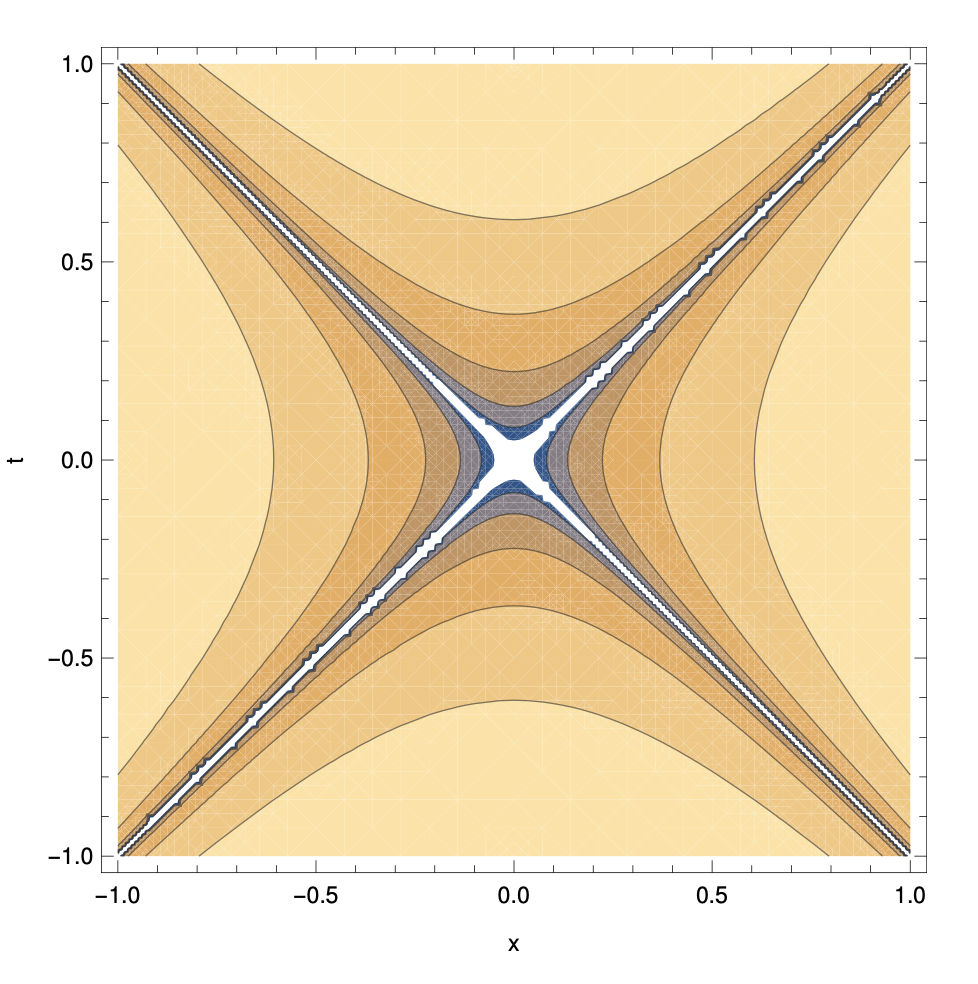
\includegraphics[scale=0.5]{Lectures/Figures/logt2x2.png}
    \caption{Plot of $\log(x^2 - t^2)$, courtesy of Luca.}
    \label{fig-logt2x2}
\end{figure}

This should not surprise us; the massless free scalar propogates at the speed of light, hence the field is very correlated with itself on the lightcone.

Remark for the formally minded: In an axiomatic approach to QFT, real-time correlators are defined by $\e \to 0$ limits of Wick rotated (analytic continuations) to imaginary time versions of the correlators, and there are perscriptions on how to handle those limits/navigate around branch cuts.

\subsection{2-Point correlator for the Free Scalar Field Theory: Momentum Space}
Restoring $m \neq 0$ and general $d$, one can evaluate the Fourier transform of the correlator of $G_W$:
\begin{equation}
    \begin{split}
        G_W(\omega, \v{k}) &= \int dt d^dx e^{-i\v{k}\cdot\v{x} - i\omega t}G_W(t, \v{x})
        \\ &= \int \frac{dtd^dxd^dk'}{(2\pi)^d}e^{i(\v{k}' - \v{k})\cdot \v{x}} e^{i(\omega - \e_{\v{k}'})t}\frac{1}{2\e_\v{k}}
    \end{split}
\end{equation}
The $x$ integral is simple and sets $\v{k'} = \v{k}$. We are then left with:
\begin{equation}
    G_W(\omega, \v{k}) = \int dt \frac{e^{i(\omega - \e_{\v{k}})t}}{2\e_\v{k}} = \frac{2\pi\delta(\omega - \e_\v{k})}{2\e_\v{k}}
\end{equation}
Thus:
\begin{equation}
    \boxed{G_W(\omega, \v{k}) = \frac{2\pi\delta(\omega - \e_\v{k})}{2\e_\v{k}}}
\end{equation}
which tells us that the Green's function only fires/resonates when $\omega = \e_\v{k}$. When we evaluated the position-space Green's function, we had the Lorentz invariance constraint. We might expect this for the momentum space version, namely:
\begin{equation}
    G_W(p^\mu) = G_W(\Lambda p^\mu).
\end{equation}
It does not look manifestly Lorentz invariant, but it is, and we will show this.

\subsection{The Feynman Correlator}
We now consider:
\begin{equation}
    G_F(t, \v{x}) = \bra{0}\mathcal{T}\set{\hat{\phi}(t, \v{x})\hat{\phi}(0, 0)}\ket{0}
\end{equation}
where $\mathcal{T}\{\cdot\}$ denotes the time-ordering operation. In other words:
\begin{equation}
    G_F(t, \v{x}) = \mathcal{T}\set{\hat{\phi}(t, \v{x})\hat{\phi}(0, \v{0})} = \Theta(t)\bra{0}\hat{\phi}(t, \v{x})\hat{\phi}(0, \v{0})\ket{0} + \Theta(-t)\bra{0}\hat{\phi}(0, \v{0})\hat{\phi}(t, \v{x})\ket{0}.
\end{equation}
With $\Theta$ the step function. This is still a measure of correlation between two points, but slightly modified. Evaluating this:
\begin{equation}
    G_F(t, \v{x}) = \Theta(t)\int \frac{d^dk}{(2\pi)^d}\frac{e^{i(\v{k} \cdot \v{x} - \e_\v{k}t)}}{2\e_\v{k}} + \Theta(-t)\int \frac{d^dk}{(2\pi)^d}\frac{e^{-i(\v{k} \cdot \v{x} - \e_\v{k}t)}}{2\e_\v{k}}.
\end{equation}
Let's compute the Fourier transform of this expression:
\begin{equation}
    \begin{split}
        G_F(\omega, \v{k}) &= \int dt d^dx e^{i(\omega t - \v{k} \cdot \v{x})}G_F(x^\mu)
        \\ &= \int dt \Theta(t)\frac{e^{i(\omega - \e_{\v{k}})t}}{2\e_\v{k}} + \Theta(-t)\frac{e^{i(\omega + \e_{\v{k}})t}}{2\e_\v{k}}
        \\ &= \int_0^\infty dt \frac{e^{i(\omega - \e_{\v{k}} + i\e)t}}{2\e_\v{k}} + \int_{-\infty}^0dt \frac{e^{i(\omega + \e_{\v{k}} - i\e)t}}{2\e_\v{k}}
        \\ &= \frac{1}{2\e_\v{k}}\left[\left.\frac{e^{i(\omega - \e_k + i\e)}}{i(\omega - \e_k + i\e)}\right|_0^\infty +\left.\frac{e^{i(\omega + \e_k - i\e)t}}{i(\omega + \e_k - i\e)t}\right|_{-\infty}^0\right]
        \\ &= \frac{1}{2\e_\v{k}}\left[\frac{-1}{i(\omega - \e_\v{k} + i\e)} + \frac{1}{i(\omega + \e_\v{k} - i\e)}\right]
        \\ &= \frac{i}{\omega^2 - (\e_\v{k} - i\e)^2}
        \\ &= \frac{i}{\omega^2 - \e_\v{k}^2 + i\tilde{\e}}
        \\ &= \frac{-i}{p^2 + m^2 - i\tilde{\e}}
    \end{split}
\end{equation}
We have again introduced the appropriate $i\e$s in order to avoid the divergences. Note that later on we will see a physical application of this; in the context of unstable particles, we have a decay that introduces some broadening of the linewidths. Also in the last lines we redefine $\tilde{\e}$ as we don't care what the small factor is, only its sign. Thus:
\begin{equation}
    \boxed{G_F(\omega, \v{k}) = \frac{-i}{p^2 + m^2 - i\tilde{\e}}}
\end{equation}
Note that this is qualitatively pretty different from the Wightman function; it does still diverge at $p^2 = -m^2$, but it is non-zero ``off-shell'', i.e. when $p^2 \neq -m^2$. Conversely, the Wightman function only fires on-shell. We will use this correlator all the time in the path integral formalism.
\newpage
\section{The Path Integral Formalism}
We could now go on from what we have used to explore how QFT can make experimental predictions - but, instead we will take a step back and explore the path integral formalism, which is a deep and widely applicable mathematical framework to understand QFT (and other fields).

\subsection{Motivating the Path Integral}
Let us return to the single particle:
\begin{equation}
    \hat{H} = \frac{\hat{P}^2}{2M} + V(\hat{Q})
\end{equation}
at position $q$ at time $0$ and $q'$ at time $T$. Classically, we could solve for the trajectory $q_{cl}(t)$ by solving $\delta S = 0$ subject to the boundary conditions.

Quantum mechanically, the procedure is quite different. We would instead compute the matrix elements:
\begin{equation}
    P(q' \text{ at time $T$}) = \abs{\bra{q'}e^{-i\hat{H}T}\ket{q}}^2
\end{equation}
This doesn't really seem like it has to do anything with the classical method of solving this same problem. On the other hand, we know that classical physics emerges from quantum physics - classical mechanics should be the limit of QM as $\hbar \to 0$. And this classical limit is indeed made clear in the path integral approach to QM. We will see that the above amplitude is related to $e^{iS[q_{cl}(t)]}$.

Advantages of the path integral formalism include:
\begin{itemize}
    \item It makes the semiclassical limit of QM manifest
    \item It involves the action $S$ rather than the Hamiltonian $\hat{H}$ (This is particularly nice from the perspective of QFT, as the action allows for Lorentz invariance to be much more easily imposed, as the action is a scalar; conversely the Hamiltonian is a four-vector, and choosing a time coordinate breaks L.I.)
    \item Streamlined calculations (e.g. correlation functions - you will see how it is possible, but tedious, to do these calculations in the ``old-fashioned'' approach, but the path integral formalism makes these much easier). Specifically, we will be computing lots of Gaussian integrals.
    \item Connections to statistical mechanics. In stat mech, we consider finite temperature fluctuations and weighing all possible field distributions weighted by their probability. This allows us to probe classical many-body physics, phase transitions etc. The path integral approach lends itself very nicely to this.
    \item Topological aspects of QFT/QM.
\end{itemize}
And there are no negatives. Just kidding. One drawback is a mathematically precise definition is difficult. But, this could be seen as a strength - the path integral gave hints towards things that were very hard to prove formally, but laid the groundwork/intuition for hard results.

\subsection{``Deriving'' the Path Integral}
Consider again the transition:
\begin{equation}
    \bra{q'}e^{-i\hat{H}T}\ket{q}.
\end{equation}
Subdivide $T$ into $N$ steps $\delta t = \frac{T}{N}$. Then:
\begin{equation}
    \bra{q'}e^{-i\hat{H}T}\ket{q} = \bra{q'}e^{-i\hat{H}\delta t} \ldots e^{-i\hat{H}\delta t} e^{-i\hat{H}\delta t}\ket{q}
\end{equation}
Now, we insert the resolution of the identity:
\begin{equation}
    \II = \int dq_i \dyad{q_i}{q_i}
\end{equation}
in between each of the exponentials. Then:
\begin{equation}
    \bra{q'}e^{-i\hat{H}T}\ket{q} = \int dq_1 \ldots dq_{N-1}\bra{q'}e^{-i\hat{H}\delta t}\ket{q_{N-1}}\bra{q_{N-1}}\ldots \ket{q_2}\bra{q_2}e^{-i\hat{H} \delta t}\ket{q_1}\bra{q_1}e^{-i\hat{H} \delta t}\ket{q}
\end{equation}
This handles nicely the $V(\hat{Q})$ term in the Hamiltonian. Now, we also insert:
\begin{equation}
    \II = \int \frac{dp_i}{2\pi} \dyad{p_i}{p_i}
\end{equation}
in each matrix element. We then have:
\begin{equation}
    \int \frac{dq_1 \ldots dq_{N-1}dp_1 \ldots dp_N}{(2\pi)^N} \braket{q'}{p_N} \bra{p_N}e^{-i\hat{H} \delta t}\ket{q_{N-1}}\ldots \braket{q_2}{p_2}\bra{p_2}e^{-i\hat{H} \delta t}\ket{q_1}\braket{q_1}{p_1}\bra{p_1}e^{-i\hat{H} \delta t}\ket{q}
\end{equation}
Now we can compute all of these factors! We have a bunch of $\braket{q}{p}$ factors, which is just the wavefunction of the momentum eigenstate:
\begin{equation}
    \braket{q}{p} = e^{iqp}.
\end{equation}
A quick way to remember this is:
\begin{equation}
    \p_q \psi_q(q) = \p_q\braket{q}{p} = \bra{q}i\hat{p}\ket{p} = ip\braket{q}{p} \implies \braket{q}{p} = e^{iqp}.
\end{equation}
For the other factors, we expand the exponentials, and use the fact that we have both a position and momentum eigenstate it can act on (from the left and right):
\begin{equation}
    \bra{p}e^{-i\hat{H}\delta t}\ket{q} \approx \bra{q}\left(1 - i\hat{H}(\hat{Q}, \hat{P})\delta t\right)\ket{p} = \braket{q}{p}\left(1 - iH(p, q)\delta t\right) = e^{-iqp}\left(1 - iH(p, q)\delta t\right) \approx e^{-ipq - iH(p, q)\delta t}
\end{equation}
We thus have the expression for the transition amplitude:
\begin{equation}
    \bra{q'}e^{-i\hat{H}T}\ket{q} = \int dq_1 \ldots dq_{N-1}\prod_{i=1}^N \int \frac{dp_i}{2\pi}\braket{q_i}{p_i}\bra{p_i}e^{-i\hat{H}\delta t}\ket{q_{i-1}}
\end{equation}
where $q_0 = q$ and $q_N = q'$. Now we apply the two calculations we did:
\begin{equation}
    \begin{split}
        \bra{q'}e^{-i\hat{H}T}\ket{q} &= \int dq_1 \ldots dq_{N-1}\prod_{i=1}^N \int \frac{dp_i}{2\pi} e^{iq_ip_i}e^{-iq_{i-1}p_i - iH(p_i, q_{i-1})\delta t}
        \\ &= \int dq_1 \ldots dq_{N-1}\prod_{i=1}^N \int \frac{dp_i}{2\pi} \exp(ip_i(q_i - q_{i-1}) - i\delta t \frac{p_i^2}{2M} - i\delta t V(q_{i-1}))
        \\ &= \int dq_1 \ldots dq_{N-1}\prod_{i=1}^N \int \frac{dp_i}{2\pi} \exp(-i\delta t \frac{1}{2M}(p_i - \frac{M}{\delta t}(q_i - q_{i-1}))^2 + \frac{i}{2}\frac{M}{\delta t}(q_i - q_{i-1})^2 - i\delta t V(q_{i-1}))
        \\ &= \int dq_1 \ldots dq_{N-1}\prod_{i=1}^N \int \frac{d\tilde{p}_i}{2\pi} \exp(-i\delta t\frac{\hat{p}_i^2}{2m})\exp(\frac{i}{2}\frac{M}{\delta t}(q_i - q_{i-1})^2 - i\delta t V(q_{i-1}))
    \end{split}
\end{equation}
where in the third equality we have completed the square, and in the fourth equality we have changed variables to $\tilde{p}_i = p_i - \frac{M}{\delta t}(q_i - q_{i-1})$. Carrying out the $\tilde{p}$ integral, we just get a constant $C$ that it independent of the $q$s, so:
\begin{equation}
    \begin{split}
        \bra{q'}e^{-i\hat{H}T}\ket{q} &= C^N\int dq_{1}\ldots dq_N \prod_{i=1}^N \exp(\frac{i}{2}\frac{M}{\delta t}(q_i - q_{i-1})^2 - i\delta t V(q_{i-1}))
        \\ &= C^N \int_{q_0=q, q_N = q'}dq_0 \ldots dq_N\exp(\sum_{i=1}^N\left[\frac{i}{2}\frac{M}{\delta T}(q_i - q_{i-1})^2 - i\delta tV(q_{i-1})\right])
    \end{split}
\end{equation}
We are left with an integral over coordinates, which we can interpret as an integral over all possible intermediate values of the coordinates. The $N \to \infty$ limit of this expression now yields the path integral. In this limit, $dt \sum_i \to \int dt$. Also, $\frac{q_{i} - q_{i-1}}{\delta t} \to \dot{q}$. Thus, taking the limit:
\begin{equation}
    \bra{q'}e^{-i\hat{H}T}\ket{q} = \tilde{C}\int \mathcal{D}q\exp(i\int_0^T dt\frac{1}{2}M\dot{q}^2 - V(q))
\end{equation}
We observe that what we integrate in the exponential is just the classical action:
\begin{equation}
    \bra{q'}e^{-i\hat{H}T}\ket{q} = \tilde{C}\int \mathcal{D}q\exp(i\int_0^T dt \mathcal{L}(q, \dot{q})) = \tilde{C}\int \mathcal{D}q \exp(iS[q, \dot{q}])
\end{equation}
Thus, the transition amplitude is simply the sum over all trajectories, weighed by a phase equal to the integral over the classical action.

In semiclassical situations, we have $S \gg \hbar = 1$. This makes extrema of the action highly important; since the action is very large, the action widely oscillates for most trajectories. But, around the classical solutions/trajectories, the phase does not vary widely (and thus the phases do not cancel), hence the path integral is dominated by trajectories very close to the classical trajectory, allowing us to recover classical physics. This is true qualitatively, and can be seen explicitly in some models, e.g. the quantum harmonic oscillator for large occupation numbers. In particle physics, we are usually not interested in semiclassical situations. We look around $\phi \approx 0$, which is a highly quantum limit. But if we hit the crystal for example, causing macroscopic osciallations, then $\phi$, and $S$ become large and we recover classical physics.

Question; how do we know this weird, infinite-dimensional measure preserves the symmetries we care about? The answer is it does not, always. This is how anomalies manifest at the quantum level.

\subsection{Computing Correlators with Path Integrals}
We start with a slightly different correlator than the one we discussed last lecture:
\begin{equation}
    \bra{q', T}\hat{Q}(t_1)\ket{q, 0}
\end{equation}
This is a one-point function; we see how to treat this with path integrals before moving onto more complicated examples. We write the above as:
\begin{equation}
    \bra{q'}e^{-i\hat{H}(T-t_1)}\hat{Q}e^{-i\hat{H}t_1}\ket{q}
\end{equation}
Following the same procedure as previous, we slice up time $T = N\delta$ and $t_1 = n\delta t$, and we get:
\begin{equation}
    \int dq_1 \ldots dq_{N-1}\bra{q'}e^{-i\hat{H}t}\ket{q_{N-1}}\ldots \bra{q_n}\hat{Q}e^{-i\hat{H}\delta t}\ket{q_{n-1}}\ldots \bra{q_1}e^{-i\hat{H}\delta t}\ket{q}
\end{equation}
so up to the $q_n$ factor,we have the same set of integrals as before, and in the continuum limit this appears as $q(t_1)$:
\begin{equation}
    \bra{q', T}\hat{Q}(t_1)\ket{q, 0} = \int \mathcal{D}q\; q(t_1)e^{iS[q, \dot{q}]}
\end{equation}
More generally, the one point function of $O(\hat{P}, \hat{Q})(t_1)$ amounts to the replacement with the number $O(p(t_1), q(t_1))$ inside the path integral.

What about two-point functions? They are slightly more interesting. A reasonable assumption would be that we get two of these factors. Lets work this out if $t_2 > t_1$:
\begin{equation}
    \bra{q', T}\hat{Q}(t_2)\hat{Q}(t_1)\ket{q, 0} = \bra{q'}e^{-i\hat{H}(T - t_2)}\hat{Q}e^{-i\hat{H}(t_2 - t_1)\hat{Q}e^{-iH t_1}}\ket{q} = \int_0^T \mathcal{D}q\; q(t_2)q(t_1)e^{iS[q, \dot{q}]}
\end{equation}
If instead $t_2 < t_1$, then we get:
\begin{equation}
    \int \mathcal{D}q q(t_2)q(t_1)e^{iS[q, \dot{q}]} = \bra{q', T}\hat{Q}(t_1)\hat{Q}(t_2)\ket{q, 0}
\end{equation}
i.e. the path integral produces \emph{time-ordered} correlation functions. Thus, in summary:
\begin{equation}
    \begin{split}
        \int \mathcal{D}q\; O(q(t_2))O(q(t_1))e^{iS[q]} 
        &= \Theta(t_2 - t_1)\bra{}\hat{O}(\hat{Q})(t_2) \hat{O}(\hat{Q})(t_1)\ket{} 
        \\ &+ \Theta(t_1 - t_2)\bra{}\hat{O}(\hat{Q})(t_1) \hat{O}(\hat{Q})(t_2)\ket{} 
        \\ &= \bra{}\mathcal{T}\{\hat{O}(\hat{Q})(t_2), \hat{O}(\hat{Q})(t_1)\}\ket{}
    \end{split}
\end{equation}
Thus, time-ordered (Feynman) correlators naturally arise in path integrals. Note that time-dependent Hamiltonians would require much more work, as the time-evolution operator would be a time-ordered exponential in this case.

One observation; operators in $\mathcal{T}\{\ldots \}$ ``commute'' in an obvious sense. Everything appearing in the above equation is symmetric in $t_1, t_2$.

What we have done here for 2-point function generalizes for higher-point functions. For example:
\begin{equation}
    \int \mathcal{D}q \; q(t_n)\ldots q(t_1) e^{iS[q, \dot{q}]} = \bra{}\mathcal{T}\{\hat{Q}(t_n)\ldots \hat{Q}(t_1)\}\ket{}.
\end{equation}
and of course we can generalize to functions of $\hat{Q}$.

For functions of $\hat{P}$, we have to keep track of this when doing the integrals over $p$ in the path integral derivation, and to first order this will give us $\sim \dot{q}$ inside of the integral.

Finally, it seems like position and time have manifestly different roles here. But its worth noting that the $\hat{Q}$s should \emph{not} be thought of as position, just coordinates in some configuration space (e.g. a quantum dot). We will apply this formalism to theories with Lorentz invariance soon.
\newpage
\section{The Path Integral Formalism, Part 2}
\subsection{Ground State Correlators}
Last class, we showed the derivation of the time evolution as a path integral:
\begin{equation}
    \bra{q'}e^{-i\hat{H}t}\ket{q} = \lim_{N \to \infty}\int dq_1 \ldots dq_N \bra{q'}e^{-i\delta t\hat{H}}\ket{q_{N-1}} \ldots \bra{q_2}e^{-i\hat{H}\delta t}\ket{q_1}\bra{q_1}e^{-i\hat{H}\delta t}\ket{q} = \int_{q(0) = q}^{q(T) = q'}\mathcal{D}q e^{iS[q]}
\end{equation}
As well as how we can evaluate (time-ordered) correlation functions\footnote{An aside - path integrals always give us the time-ordered correlation functions, but these objects contain the information necessary to get other correlation functions.} using this machinery:
\begin{equation}
    \int_{q(0) = q}^{q(T) = q'} \mathcal{D}q q(t_1)q(t_2)\ldots e^{iS[q]} = \bra{q', T}\mathcal{T}\{\hat{Q}(t_1), \hat{Q}(t_2), \ldots \} \ket{q, 0}
\end{equation}

To connect this back to what we were doing previously, we are mostly interested in correlations in the ground state (which we will later see will be related to scattering amplitudes). So, today we will look at ground state correlators/excitations above the ground state. In this case, things simplify, as we will soon see. Rather than looking at:
\begin{equation}
    \bra{q', t_f}\hat{Q}(\bar{t})\ket{q, t_i} = \bra{q'}e^{-i\hat{H}(t_f - \bar{t})}\hat{Q}e^{-i\hat{H}(\bar{t} - t_i)}\ket{1} = \int_{q(t_i) = q}^{q(t_f) = q'}\mathcal{D}q e^{i\int_{t_i}^{t_f}dt L(q, t)}q(\bar{t})
\end{equation}
We would like to look at:
\begin{equation}
    \bra{0}\hat{Q}(\bar{t})\ldots \ket{0}.
\end{equation}
The issue; for most field theories (e.g. interacting field theories), we do not know what the ground state $\ket{0}$ is! But, we do know that (by definition) it is the lowest energy state. Let us focus on $e^{i\hat{H}t_i}\ket{q}$ factor. If we take $t_i \to -\infty(1 -i\e)$, then this factor will become $e^{iE_0 t_i}\ket{0}\braket{0}{q}$, i.e. only the contribution from the ground state will survive (to derive that expression explicitly, insert a complete basis of energy eigenstates, and see how all terms proportional to $e^{-\e\infty(E_i - E_0)} \to 0$ (unless $E_i = E_0$)). Doing the same on the bra, we consider $\bra{q'}e^{-i\hat{H}t_f}$ and send $t_f \to \infty(1 - i\e)$, again exponentially suppressing everything but the ground state, and giving $\braket{q'}{0}\bra{0}e^{-iE_0 t_f}$. The bottom line; up to some factors, we have:
\begin{equation}
    \bra{0}\mathcal{T}\{\hat{Q}(t_1), \hat{Q}(t_f)\}\ket{0} \propto \int \mathcal{D}q q(t_2)q(t_1)e^{i\int_{-\infty(1-i\e)}^{\infty(1-i\e)}dt L(q, t)}
\end{equation}
An interesting observation is that the boundary conditions no longer matter in the time dependence of the correlation! They only matter for the normalization, which we fix now. Let us set the norm of the vacuum to be one:
\begin{equation}
    \bra{0}\mathbb{I}\ket{0} = 1
\end{equation}
Which then tells us that:
\begin{equation}
    \bra{0}\mathcal{T}\{\hat{Q}(t_1), \hat{Q}(t_2)\}\ket{0} = \frac{\int \mathcal{D}q q(t_1)q(t_2)e^{i\int_{-\infty(1-i\e)}^{\infty(1-i\e)}dt L(q, t)}}{\int \mathcal{D}q e^{i\int_{-\infty(1-i\e)}^{\infty(1-i\e)}dt L(q, t)}}
\end{equation}
By looking at \emph{ratios} of path integrals, we don't have to worry about the factors that we had lying around. Srednicki says that by normalization fixing, we can choose the measure such the ``empty'' path integral in the denominator can be normalized to one, but this is a matter of convention. In any case, we now have a recipe for computing things in the path integral formalism! 

From now on we drop the $ie$s in our notation, until we need to explicitly use them.

\subsection{Generating Functionals}
In some cases (e.g. the simple harmonic oscillator), instead of computing the correlation functions one by one, we can construct one general object - namely, the \emph{generating functional} - from which all of the correlation functions can be derived. Let us define:
\begin{equation}
    Z[f] = \int \D q e^{iS[q] + i\int dt f(t)q(t)}
\end{equation} 
By taking functional derivatives $\frac{\delta}{\delta f(t_1)}$, we can generate correlators involving $\hat{Q}(t_1)$. Let us study:
\begin{equation}
    \fd{}{f(t_1)}Z[f] = \int \D q e^{iS[q] + i\int dt f(t)q(t)}\fd{}{f(t_1)}[i\int dt f(t)q(t)].
\end{equation}
The functional derivative of a function w.r.t itself is just the delta function which fires only when the arguments are the same:
\begin{equation}
    \fd{f(t)}{f(t_1)} = \delta(t - t_1)
\end{equation}
so then the above becomes:
\begin{equation}
    \fd{}{f(t_1)}Z[f] = \int \D q (iq(t_1))e^{iS + i\int dt f(t)q(t)}
\end{equation}
Which is not quite what we want, but let us consider taking a ratio, and setting the source term to zero after taking the derivative:
\begin{equation}
    \left.\frac{1}{Z}\frac{1}{i}\fd{f(t_1)}Z\right|_{f = 0} = \frac{\int \D q q(t_1)e^{iS}}{\int \D q e^{iS}} = \bra{0}\hat{Q}(t_1)\ket{0}
\end{equation}
Let's now consider more derivatives!
\begin{equation}
    \left.\frac{1}{Z}\frac{1}{i}\fd{}{f(t_1)}\frac{1}{i}\fd{}{f(t_2)}Z[f]\right|_{f=0} = \frac{\int \D q q(t_1)q(t_2)e^{iS}}{\int \D q e^{iS}} = \bra{0}\mathcal{T}\{\hat{Q}(t_1), \hat{Q}(t_2)\}\ket{0}
\end{equation}

$Z[f]$ is a very rich object (a functional of a functional), which makes it generically hard to compute (but we can for free QFTs, and the harmonic oscillator). An observation; we can write the above formulas as:
\begin{equation}
    \left.\frac{1}{i}\fd{}{f(t_1)}\log Z[f]\right|_{f=0}
\end{equation}
For higher derivatives, we have:
\begin{equation}
    \left.\frac{1}{i}\fd{}{f(t_1)}\frac{1}{i}\fd{}{f(t_2)}\log Z[f]\right|_{f=0} = \frac{1}{i}\fd{}{f(t_2)}\frac{\int \D q q(t_1)e^{iS + i\int fq}}{Z[f]}
\end{equation}
Now that now there are two places where the functional derivative can hit. When it hits the numerator, we get a two-point function as before, when it hits the denominator, we get something that looks like a one-point function. Let's spell this out:
\begin{equation}
    \begin{split}
        \left.\frac{1}{i}\fd{}{f(t_1)}\log Z[f]\right|_{f=0} &= \frac{\int \D q q(t_1)q(t_2)e^{iS}}{\int \D q e^{iS}} - \frac{\int \D q(t_1)e^{iS}}{Z[0]}\frac{\int \D q q(t_2)e^{iS}}{Z[0]}
        \\ &= \bra{0}\mathcal{T}\{\hat{Q}(t_1), \hat{Q}(t_2)\}\ket{0} - \bra{0}\hat{Q}(t_1)\ket{0}\bra{0}\hat{Q}(t_2)\ket{0}
        \\ &= \bra{0}\mathcal{T}\{\hat{Q}(t_1), \hat{Q}(t_2)\}\ket{0}_C
    \end{split}
\end{equation}
where $Z[0] = \int \D q e^{iS}$. The object above is a connected correlator. Thus we say that $\log Z$ generates ``correlated'' correlation functions. Why is this important? Well, suppose $\hat{Q}$ was equal to 6 everywhere. Then the raw two-point function would just be $6^2 = 36$. Thus, looking at the connected correlation function removes this background, and actually tells us about the important correlations; this is intimately tied to covariance in probability theory. In the context of scattering, connected correlators tell us about nontrivial scattering processes.

\subsection{Path Integral for the Harmonic Oscillator}
The action for the simple harmonic oscillator is:
\begin{equation}
    S = \int dt \frac{1}{2}\dot{q}^2 - \frac{1}{2}mq^2
\end{equation}
Let's try to compute $Z$:
\begin{equation}
    Z[f] = \int \D q e^{iS + \int dt f(t)q(t)}
\end{equation}
Since we have time translation invariance, it will be convenient to study this object in frequency space. Let us define:
\begin{equation}
    q_\omega = \int dt e^{i\omega t}q(t)
\end{equation}
where the inverse fourier transform is then:
\begin{equation}
    q(t) = \int \frac{d\omega}{2\pi}e^{-i\omega t}q_\omega
\end{equation}
Plugging this into the action, we can perform the integral over $t$, then use the resulting delta functions to carry out one of the two $\omega$ integrals, and we end up with:
\begin{equation}
    S = \int \frac{d\omega}{2\pi}\frac{1}{2}(\omega^2 - m^2)q_\omega q_{-\omega}
\end{equation}
with $q_{-\omega} = q_\omega^*$. Now we study the source integral:
\begin{equation}
    \int dt f(t) q(t) = \int \frac{d\omega_1}{2\pi}\frac{d\omega_2}{2\pi}\int dt e^{-i(\omega_1 + \omega_2)t}f_{\omega_1}q_{\omega_2} = \int \frac{d\omega}{2\pi}f_\omega q_{-\omega} = \int \frac{d\omega}{2\pi}\frac{1}{2}\left(f_{\omega}q_{-\omega} + f_{-\omega}q_{\omega}\right)
\end{equation}
where we symmetrize in the last equality. We are now ready to compute the beast that is the functional integral. Spelling out the exponents, we have:
\begin{equation}
    Z[f] = \int \D q \exp(i\left[\int \frac{d\omega}{2\pi}\frac{1}{2}(\omega^2 - m^2)q_{\omega}q_{-\omega} + \frac{1}{2}(f_{\omega}q_{-\omega} + q_\omega f_{-\omega})\right])
\end{equation}
Now completing the square:
\begin{equation}
    Z[f] = \int \D q \exp(i\left[\int \frac{d\omega}{2\pi} \frac{1}{2}(\omega^2 - m^2)(q_\omega + \frac{1}{\omega^2 - m^2}f_\omega)(q_{-\omega}  + \frac{1}{\omega^2-m^2}f_{-\omega}) - \frac{1}{2}\frac{1}{\omega^2 - m^2}f_{\omega}f_{-\omega}\right])
\end{equation}
Let us shift our $q$ variable $q_\omega \to \bar{q}_\omega = q_\omega + \frac{1}{\omega^2 - m^2}f_\omega$. Then our path integral becomes:
\begin{equation}
    Z[f] = \int \D \bar{q}\exp(i\left[\frac{1}{2}\int \frac{d\omega}{2\pi}(\omega^2 - m^2)\bar{q}_\omega \bar{q}_{\omega}\right])\exp(-\frac{i}{2}\int \frac{d\omega}{2\pi}\frac{1}{\omega^2 - m^2}f_\omega f_{-\omega})
\end{equation}
Note that the path integral has decoupled from the source part! Since the first piece is just the generating functional without sources, so $Z[f]$ decouples to $Z[0]$ times a fairly simple functional of our source function:
\begin{equation}
    Z[f] = Z[0] \cdot  \exp(-\frac{i}{2}\int \frac{d\omega}{2\pi}\frac{1}{\omega^2 - m^2}f_\omega f_{-\omega})
\end{equation}
The logarithm is even simpler:
\begin{equation}
    \log Z[f] = -\frac{i}{2}\int \frac{d\omega}{2\pi}\frac{1}{\omega^2 - m^2}f_\omega f_{-\omega} \left(+ \log Z[0]\right)
\end{equation}
The $Z[0]$ part is independent of our probe $f$, so it is irrelavant for the calculation of our correlation functions - let's look at some of them now!
\begin{equation}
    \left.\fd{}{f}\log Z \right|_{f=0} = \bra{0}\hat{Q}(t_1)\ket{0} = 0
\end{equation}
We see this as we take the derivative of one of the $f$s, the other remains and gets set to zero, thus making the one-point function vanish. Let's now look at two-point functions, but first let's go back to the time domain:
\begin{equation}
    \log Z[f] = -\frac{i}{2} \int dtdt'\int \frac{d\omega}{2\pi}e^{i\omega(t - t')}\frac{1}{\omega^2 - m^2}f(t)f(t')
\end{equation}
Let us call the frequency integral above $G(t - t')$
\begin{equation}
    \log Z[f] = -\frac{i}{t}\int dtdt' G(t - t')f(t)f(t')
\end{equation}
Now looking at the connected correlation function (which is equal to the bare two-point function, since the one-point functions vanish):
\begin{equation}
    \begin{split}
        \bra{0}\mathcal{T}\{\hat{Q}(t_1), \hat{Q}(t_2)\}\ket{0} &= \frac{1}{i}\fd{}{f(t_2)}\frac{1}{i}\fd{}{f(t_1)}\log Z
        \\ &= \frac{1}{i}\fd{}{f(t_2)}\left(-\frac{1}{2}\right)\int dtdt' G(t-t')\fd{}{f(t_1)}(f(t)f(t'))
        \\ &= \frac{1}{i}\fd{}{f(t_2)}\left(-\frac{1}{2}\right)\int dtdt' G(t-t')\left(\delta(t - t_1)f(t') + \delta(t' - t_1)f(t)\right)
        \\ &= \frac{i}{2}\fd{}{f(t_2)}\left(\int dt' G(t_1 - t')f(t') + \int dt G(t - t_1)f(t)\right)
    \end{split}
\end{equation}
Now we take the second derivative, which is easy, as there is only one $f$ to hit in each term:
\begin{equation}
    \begin{split}
        \bra{0}\mathcal{T}\{\hat{Q}(t_1), \hat{Q}(t_2)\}\ket{0} &= \frac{i}{2}\left(G(t_1 - t_2) + G(t_2 - t_1)\right)
    \end{split}
\end{equation}
Since $G$ is symmetric in its argument, we find:
\begin{equation}
    \bra{0}\mathcal{T}\{\hat{Q}(t_1), \hat{Q}(t_2)\}\ket{0} = iG(t_2 - t_1)
\end{equation}
Since the two-point function is just the Feynman's Green's function, we ave;
\begin{equation}
    G_F(t_2 - t_1) = iG(t_2 - t_1)
\end{equation}
On Thursday we evaluate this explicitly, and we will have to be careful about poles (we will see the return of the $i\e$s). We will then move onto free quantum field theories, where connected higher point functions are then easily computed.
\newpage
\section{Wick's Theorem, Path Integral for Free Scalar Field Theory}
\subsection{Review}
We computed the path integral with sources (also known as the generating functional) for the SHO, with action:
\begin{equation}
    S = \int dt \frac{1}{2}\dot{q}^2 - \frac{1}{2}\omega^2q^2 = \int \frac{d\omega}{2\pi}\frac{1}{2}(\omega^2 - m^2)q_\omega q_{-\omega}
\end{equation}
which gave the generating functional:
\begin{equation}
    Z[f] = \int \D q e^{iS + \int dt f(t)q(t)} = Z[0]\exp(-\frac{i}{2}\int \frac{d\omega}{2\pi}\frac{1}{\omega^2 - m^2}f_\omega f_{-\omega})
\end{equation}
the logarithm which gives:
\begin{equation}
    \log Z[f] = -\frac{i}{2}\int \frac{d\omega}{2\pi}\frac{1}{\omega^2 - m^2}f_\omega f_{-\omega} = \frac{i}{2}\int dtdt'(-1)\int \frac{d\omega}{2\pi} \frac{e^{-i\omega(t-t')}}{\omega^2 - m^2} f_\omega f_{-\omega} = \frac{i}{2}\int dt'dt'(-1)G(t-t')f_\omega f_{-\omega}
\end{equation}

We can then generate (connected) correlators by taking functional derivatives $\fd{}{f(t)}$ and then setting the source to $f = 0$. For example:
\begin{equation}
    \bra{0}\mathcal{T}\set{\hat{Q}(t_1), \hat{Q}(t_2)}\ket{0} = \left.\frac{1}{i}\fd{}{f(t_1)}\frac{1}{i}\fd{}{f(t_2)}\log Z[f] \right|_{f=0} = -iG(t_1 - t_t) = G_F(t_1 - t_2)
\end{equation}

\subsection{Evaluating the Green's Function}
Now, let's evaluate the fourier transform:
\begin{equation}
    G(t) = -\int \frac{d\omega}{2\pi}\frac{e^{i\omega t}}{\omega^2 - m^2 + i\e}
\end{equation}
We were dropping the $i\e$s previously, but when evaluating this integral, it becomes relevant for locating the poles of the function. So, we re-introduce it here (we know what the correct perscription of the poles for the Feynman correlator is).

The poles are located at $\omega_\pm = \pm \sqrt{m^2 - i\e}$. They are close to $\pm m$, but they are shifted from the real axis. How do we treat these $i\e$? We don't care about the magnitude, only that it is a positive number. We consider a Taylor expansion:
\begin{equation}
    \omega_\pm = \pm m\sqrt{1 - \frac{i\e}{m}} = \pm m(1 - i\e)
\end{equation}
where we have neglected factors of $m, 2$ as we don't care about the magnitude of $\e$, only its sign. Hence, the poles are at:
\begin{equation}
    \omega_\pm = \pm m(1 - i\e)
\end{equation}
which when sketched graphically:
\begin{center}
    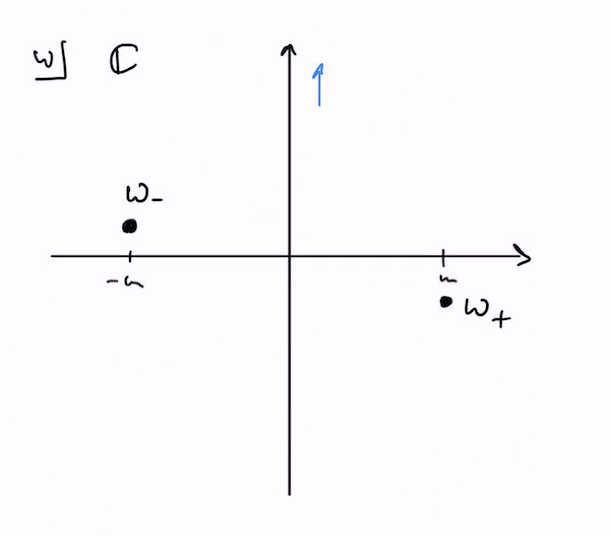
\includegraphics[scale=0.8]{Lectures/Figures/Feynmanpoles.png}
\end{center}

How do we perform this integral? It depends on whether $t$ is positive or negative. If $t < 0$, then we want to close the contour in the lower half plane. Why this choice? We are concretely interested in the integral from $-\infty$ to $\infty$, i.e. $C_1^A$. For this, we like to have a closed contour in the complex plane to carry out the integrals using residue theorems. We use Jordan's lemma. The integral over the semicircular part $C_1^B$ vanishes - as long as $\omega$ has a negative imaginary part, when we push the $C_1^B$ to be a sufficiently large arc to infinity ($e^{i\omega t} = e^{\omega t} = e^{-\abs{t}\omega} \stackrel{\omega\to\infty}{\to} 0$). So, this total closed contour is precisely equal to the integral over the real line.

\begin{center}
    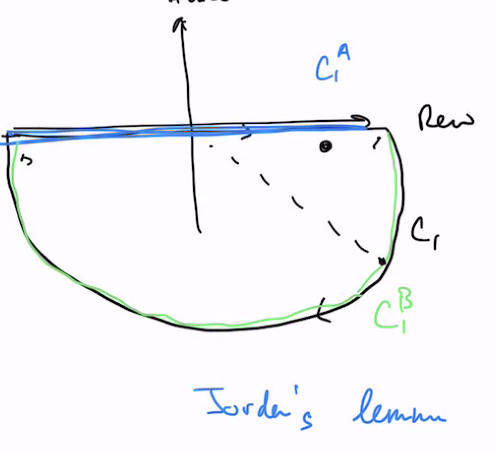
\includegraphics[scale=0.8]{Lectures/Figures/lowerhalfcontour.png}
\end{center}

By the residue theorem:
\begin{equation}
    G(t) = -\int_{C_1}\frac{d\omega}{2\pi}\ldots = 2\pi i \text{Res}(\frac{1}{2\pi}\frac{e^{-i\omega t}}{(\omega - \omega_+)(\omega - \omega_-)}, \omega \to \omega_+) = i\frac{e^{-i\omega_+ t}}{\omega_+ - \omega_-} = i\frac{e^{-im\abs{t}}}{2m}
\end{equation}

If $t > 0$, we close the contour in the upper-half plane:
\begin{center}
    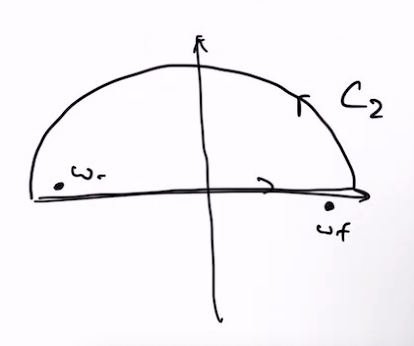
\includegraphics[scale=0.8]{Lectures/Figures/upperhalfcontour.png}
\end{center}
So:
\begin{equation}
    G(t) = -\int_{C_2}\frac{d\omega}{2\pi}\ldots = -2\pi i \text{Res}(\frac{1}{2\pi}\frac{e^{i\omega t}}{(\omega - \omega_+)(\omega - \omega_-)}, \omega \to \omega_-) = -i\frac{e^{i\omega_-t}}{\omega_- - \omega_+} = i\frac{e^{-imt}}{2m} = i\frac{e^{-im\abs{t}}}{2m}
\end{equation}

\subsection{Higher-Point Functions and Wick's Theorem}
What about higher point functions? Let's study the 4-point function. (All odd higher point functions vanish due to symmetry).

\begin{equation}
    \bra{0}\mathcal{T}\{\hat{Q}(t_1)\hat{Q}(t_2)\hat{Q}(t_3)\hat{Q}(t_4)\}\ket{0} = \left.\frac{1}{Z}\frac{1}{(i)^4}\fd{}{f(t_1)}\fd{}{f(t_2)}\fd{}{f(t_3)}\fd{}{f(t_4)} Z[f]\right|_{f=0}
\end{equation}

The connected 4-point function (denoting $\p_i = \fd{\delta}{\delta f(t_i)}$):
\begin{equation}
    \begin{split}
        \p_{1}\p_{2}\p_{3}\p_{4}\log Z &= \p_1\p_2\p_3\left(\frac{\p_4 Z}{Z}\right) 
        \\ &= \p_1\p_2\left(\frac{\p_3\p_4 Z}{Z} - \frac{\p_3 Z}{Z}\frac{\p_4 Z}{Z}\right)
        \\ &= \left.\p_1\left(\frac{\p_2\p_3\p_4 Z}{Z} - \frac{\p_3\p_4 Z}{Z}\frac{\p_2 Z}{Z} - \frac{\p_2\p_3 Z \p_4 Z}{Z^2} - \frac{\p_3 Z\p_2\p_4 Z}{Z^2} + 2\frac{\p_2Z \p_3 Z\p_4 Z}{Z^2}\right)\right|_{f=0}
        \\ &= \frac{\p_1\p_2\p_3\p_4 Z}{Z} - \frac{\p_3\p_4 Z}{Z}\frac{\p_1\p_2 Z}{Z} - \frac{\p_2\p_3 Z \p_1\p_4 Z}{Z^2} - \frac{\p_1 \p_3 Z \p_2 \p_4 Z}{Z^2}
    \end{split}
\end{equation}
An observation; only terms with an even number of derivatives will survive when we set $f = 0$, which we use in the last equality (we discard all terms with an odd number of derivatives). We use this observation in the last equality. Thus:
\begin{equation}
    \begin{split}
        &\bra{0}\mathcal{T}\{\hat{Q}(t_1)\hat{Q}(t_2)\hat{Q}(t_3)\hat{Q}(t_4)\}\ket{0}_C 
        \\ &= \bra{0}\mathcal{T}\{\hat{Q}(t_1)\hat{Q}(t_2)\hat{Q}(t_3)\hat{Q}(t_4)\}\ket{0} - \bra{0}\hat{Q}(t_4)\hat{Q}(t_3)\ket{0}\bra{0}\hat{Q}(t_2)\hat{Q}(t_1)\ket{0} - \ldots
        \\ &= \bra{0}\mathcal{T}\{\hat{Q}(t_1)\hat{Q}(t_2)\hat{Q}(t_3)\hat{Q}(t_4)\}\ket{0} - G_F(t_4-t_3)G_F(t_2-t_1) - G_F(t_4-t_2)G_F(t_3-t_1) - G_F(t_4-t_1)G_F(t_3-t_2)
    \end{split}
\end{equation}
i.e. the connected correlation function is just the 4 point function minus all possible pairs of contractions. Note that this result is true beyond the simple harmonic oscillator (there was no dependence on the actual form of $Z$ here), and is true of any theory where there is a $Q \leftrightarrow -Q$ $\mathbb{Z}_2$ symmetry.

For the SHO (and ``Gaussian'' theories more generally), we found that $\log Z \propto f^2$, i.e. all \emph{connected} higher-point functions vanish. This gives us a way to express the four-point function in terms of the two-point functions:
\begin{equation}
    \bra{0}\mathcal{T}\{\hat{Q}(t_1)\hat{Q}(t_2)\hat{Q}(t_3)\hat{Q}(t_4)\}\ket{0} = G_F(t_4-t_3)G_F(t_2-t_1) + G_F(t_4-t_2)G_F(t_3-t_1) + G_F(t_4-t_1)G_F(t_3-t_2)
\end{equation}
Or, phrased another way; in terms of all contractions. In PS3, we showed this using a very different (brute force) approach. The proof we did here is much easier to generalize to higher-point functions. This is generally known as \emph{Wick's theorem}, which (if the connected correlation functions vanish) we can express higher point functions as all contractions of lower-degree correlation functions.

\subsection{Path Integral for the Free Scalar}
Our action for the free scalar field is:
\begin{equation}
    S = \int dt \frac{1}{2}\dot{q}^2 - \frac{1}{2}m^2q^2 \to S = \int dt d^dx \frac{1}{2}(-\p_\mu \phi)^2 - \frac{1}{2}m^2\phi^2
\end{equation}
Where the distinction from the SHO case is we have changed from the classical coordinate $q(t)$ to the classical field $\phi(t, \v{x})$, or in terms of quantum operators, from the operator $\hat{Q}(t)$ to the field operator $\hat{\phi}(t, \v{x})$. 

We again consider a generating functional and sources, where we promote the source $f(t)$ in the SHO case to the source $J(t, \v{x}) = J(x)$. Thus, we have the action plus source:
\begin{equation}
    S + \int d^{d+1}x J(x)\phi(x).
\end{equation}
The path integral is an integral over all histories $\phi(t, \v{x})$. We see this in the integral $\int \mathcal{D}\phi$ for the generating functional:
\begin{equation}
    Z[J] = \int \D \phi e^{i\int d^{d+1}L + J(x) \phi(x)}
\end{equation}
We can generate correlators like before, e.g.:
\begin{equation}
    \bra{0}\mathcal{T}\set{\hat{\phi}(t_1, \v{x}_1)\hat{\phi}(t_2, \v{x}_2)}\ket{0} = \left.\frac{1}{Z}\frac{1}{i}\fd{}{J(x_1)}\frac{1}{i}\fd{}{J(x_2)}Z[J]\right|_{J=0}.
\end{equation}
The free scalar field will turn out to have a very similar solution to that of the SHO (both are ``Gaussian''):
\begin{equation}
    S + \int d^{d+1}J(x)\phi(x) = \int \frac{d^{d+1}p}{(2\pi)^{d+1}}\left(-\frac{1}{2}\right)(p^2 + m^2)\phi_p\phi_{-p} + \frac{1}{2}(J_p\phi_{-p} + \phi_pJ_{-p})
\end{equation}
Where $p^2 = -(p_0)^2 + \v{p}^2 = -\omega^2 + \v{p}^2$ and $\phi_p = \int d^{d+1}x e^{-ip_\mu x^\mu}\phi(x)$ and similarly for $J_p$. Like we did for the SHO, we complete the square:
\begin{equation}
    \begin{split}
        S[\phi] + \int d^{d+1}J(x)\phi(x) = \int \frac{d^{d+1}p}{(2\pi)^{d+1}} \left(-\frac{1}{2}\right)(p^2+ m^2)\left(\phi_p - \frac{1}{p^2 + m^2}J_p\right)\left(\phi_{-p} - \frac{1}{p^2 + m^2}J_{-p}\right) + \frac{1}{2}J_p\frac{1}{p^2 + m^2}J_{-p}
        \\ &= S[\bar{\phi}] + \int \frac{d^{d+1}p}{(2\pi)^{d+1}}\frac{1}{2}J_p\frac{1}{p^2 + m^2}J_{-p}
    \end{split}
\end{equation}
To compute $Z$, we perform the change of variable $\phi_p \to \bar{\phi}_p = \phi_p - \frac{1}{p^2 + m^2}J_p$, so:
\begin{equation}
    Z[J] = \int \D\bar{\phi}e^{iS[\bar{\phi}]}e^{i\int \frac{d^{d+1}p}{(2\pi)^{d+1}}\frac{1}{2}J_p\frac{1}{p^2 + m^2}J_{-p}} = Z[0]\exp(\frac{i}{2}\int \frac{d^{d+1}p}{(2\pi)^{d+1}}J_p\frac{1}{p^2 + m^2}J_{-p})
\end{equation}
So we've basically solved the free scalar QFT, in the sense that we have a generating functional for it. As with the QHO, we observe that $\log Z[J]$ is very simple:
\begin{equation}
    \log Z[J] = \log Z[0] + \frac{i}{2}\int \frac{d^{d+1}p}{(2\pi)^{d+1}}J_p\frac{1}{p^2 + m^2}J_{-p} = \log Z[0] + frac{i}{2}\int \frac{d^{d+1}p}{(2\pi)^{d+1}}J_pG_F(p)J_{-p}
\end{equation}
i.e. since $\log Z[J] \sim J^2$, so we have that higher connected correlation functions ($n > 2$) vanish and Wick's theorem applies! Thus higher point functions can be written as contractions, which will just be functions of the two-point functions (all higher-point functions are determined by the two-point functions). I.e.:
\begin{equation}
    \bra{0}\mathcal{T}\{\hat{\phi}_1, \hat{\phi}_2, \hat{\phi}_3, \hat{\phi}_4\}\ket{0} = \avg{12}\avg{34} + \avg{13}\avg{24} + \avg{14}\avg{23}
\end{equation}

In position space:
\begin{equation}
    \log Z[J] = \frac{i}{2}\int d^{d+1}xd^{d+1}x'\left(\int \frac{d^{d+1}p}{(2\pi)^{d+1}}\frac{e^{-ip(x-x')}}{p^2 + m^2 - i\e}\right) J(x)J(x') = \frac{i}{2}\int d^{d+1}xd^{d+1}x' G_F(x-x')J(x)J(x')
\end{equation}
so we recover the same result we found in the Hamiltonian approach using the path integral approach. To expand slightly on the last point, the Feynman's Green function is the time-ordered correlation function:
\begin{equation}
    G_F(x -x') = \bra{0}\mathcal{T}\{\hat{\phi}(x), \hat{\phi}(x')\}\ket{0} = \left.\frac{1}{Z}\frac{1}{i}\fd{}{J(x)}\frac{1}{i}\fd{}{J(x')} \log Z\right|_{J=0} = -i\int \frac{d^{d+1}p}{(2\pi)^{d+1}}\frac{e^{-ip(x-x')}}{p^2 + m^2 - i\e}
\end{equation}
where in the second-to-last equality we note that for two-point functions, connected correlation functions are the unconnected correlation functions because the one-point functions vanish.

\subsection{Looking Ahead}
This is a great starting point; we have a fully solved (free) QFT. But, the world would be pretty uninteresting if it was free. We will start to look at interactions, which are generally unsolvable. But for sufficiently weak interaction, a lot of our machinery will come in useful.

As a teaser, we can consider a $\phi^3$ term:
\begin{equation}
    S = S_{\text{free}} + \lambda\int \phi^3
\end{equation}
which breaks the $\mathbb{Z}_2$ symmetry, so we see that three-point functions will now be nonzero:
\begin{equation}
    \bra{0}\hat{\phi}_1\hat{\phi}_2\hat{\phi}_3 \sim \lambda \neq 0.
\end{equation}
How do we attack this? We will consider:
\begin{equation}
    \int \D \phi e^{iS_{\text{free}}}e^{iS_{text{int}}}
\end{equation}
with $e^{iS_{text{int}}} \approx 1+ i\lambda \int \phi^3$ and roughly this corresponds to taking expectations of the interactions with the free theory:
\begin{equation}
    \bra{0}\hat{\phi}_1\hat{\phi}_2\hat{\phi}_3 \approx \bra{0}\phi\phi\phi \left(i\lambda \int \phi^3 \right)\ket{0} \neq 0 
\end{equation}
\newpage
\section{Noether's Theorem and Currents}

\subsection{Motivation + Review of Symmetries and Correlation Functions}
Today, we will change gears slightly and talk about a very general result in Quantum Field Theory; namely, Noether's Theorem. We will discuss operators known as currents, and we will discuss Ward Identities, which are a powerful consequence of Noether's theorem. These results will be true for any quantum field theory (they will be based on symmetries) - over the past few weeks, we've built up computational tools for doing perturbative calculations in specific QFTs, but the tools we develop today will be highly general. In fact, symmetries are one of the few non-perturbative tools in QFT.

We've seen this manifest in our discussion of correlation functions; for example, the translation invariance implies that 2-point functions only depend on the difference of spacetime coordinates:
\begin{equation}
    \bra{0}\hat{\phi}(x^\mu_1)\hat{\phi}(x^\mu_2)\ket{0} = \bra{0}\hat{\phi}(x^\mu_1 - x^\mu_2)\ket{0}
\end{equation}
And Lorentz invariance tells us that the Wightman function only depends on the spacetime interval (a stronger result than depending on the $d+1$ differences of spacetime coordinates):
\begin{equation}
    G(x^\mu) = \bra{0}\hat{\phi}(x^\mu)\hat{\phi}(0)\ket{0} = G(x^2)
\end{equation}
We also saw that $\hat{\phi} \leftrightarrow -\hat{\phi}$ $\mathbb{Z}_2$ symmetry implies that odd $n$-point functions vanish:
\begin{equation}
    \bra{0}\hat{\phi}\ket{0} = \bra{0}\hat{\phi}^{2n+1}\ket{0} = 0.
\end{equation}

Today, we will see another consequence of symmetry; the existence of \emph{currents} $\hat{j}^\mu$, which are local operators satisfying a special property (Ward Identities). This whole chapter in our discussion of QFT will be highly general - it will not rely on the theory being free/Gaussian, or weakly interacting. We can have an arbitrarily complex quantum field theory, and so long as they have symmetries these results will apply! In Srednicki, the relevant sections are 22, 24.

\subsection{Definition and Group Structure of Symmetries}
When we discussed Lorentz invariance, we discussed how symmetries form a group. To generalize the discussion a little bit, we consider an action $S[\phi_a]$ for several scalar fields $\phi_a$ ($a = 1, 2, \ldots, N$). Let's assume that it is invariant under a transformation:
\begin{equation}
    \phi_a \to \phi_a'(\phi_b)
\end{equation}
i.e. the action for the transformed field is equal to the action for the original field:
\begin{equation}
    S[\phi_a'] = S[\phi_a]
\end{equation}
This is (the definition of) a symmetry of the theory.

Such symmetries form groups, which means that (based on the group axioms):
\begin{itemize}
    \item The composition of two symmetries is a symmetry
    \item There is an identity, namely the identity transformation $\phi_a' = \phi_a$
    \item For each symmetry, there exists an inverse.
\end{itemize}
It's worth noting that it is a currently active field of research to extend this notion of symmetry beyond groups (so-called ``non-invertible'' or ``categorical'' symmetries), but for the purposes of this course we will consider symmetries with group structure only.

Symmetries can be \emph{discrete} or \emph{continuous}. An example of the former is reflection symmetry, an example of the latter is translation. This is whether the group describing the symmetry is discrete or continuous. Continuous symmetries have infinitesimal versions, while discrete ones do not (this will have relevance later in our discussion of Noether's theorem). Symmetries can also be \emph{internal}, or \emph{spacetime}, which are symmetries that act on fields themselves vs. on the coordinates directly. This is pretty abstract, so let's go through examples.

\subsection{Examples of Symmetry}
\subsubsection*{$\phi^4$ scalar field theory}
Consider the scalar $\phi^4$ theory, which we have seen previously:
\begin{equation}
    S[\phi] = \int d^4x \frac{1}{2}(\p\phi)^2 + \frac{1}{2}m^2\phi^2 + \lambda \phi^4
\end{equation}
This theory has lots of symmetries! One example is:
\begin{equation}
    \phi \to \phi' = -\phi.
\end{equation}
which is evidently a symmetry of the action $S[-\phi] = S[\phi]$ as it only depends on even powers of $\phi$. This (as our previous discussion) tells us that odd $n$-point functions vanish (even in highly interacting theories where such functions may be exceptionally difficult to compute)! This is a discrete, internal symmetry, with symmetry group $\mathbb{Z}_2 = \set{1, -1}$ where $1$ corresponds to the identity and $-1$ corresponds to flipping the sign of $\phi$. The group multiplication rules are very simple:
\begin{equation}
    1 \cdot 1 = -1 \cdot -1 = 1, \quad 1 \cdot -1 = -1 \cdot 1 = -1.
\end{equation}
This symmetry can be broken by introducing odd powers into the action, e.g. $\tilde{\lambda}\phi^3$.

\subsubsection*{Two scalar fields}
Consider an action with two scalar fields $\phi_{a=1,2}$. Consider the Lagrangian density:
\begin{equation}
    \mathcal{L} = -\frac{1}{2}(\p_\mu \phi_1)^2 - \frac{1}{2}m^2\phi_1^2 --\frac{1}{2}(\p_\mu \phi_2)^2 - \frac{1}{2}m^2\phi_2^2 = -\frac{1}{2}(\phi_\mu \phi_a)^2 - \frac{1}{2}m^2(\phi_a)^2
\end{equation}
with $\phi_a^2 = \phi_1^2 + \phi_2^2$. This theory is invariant under ``rotations'' of the fields (NOT a spacetime rotation - but considering a 2-D space in $\phi_1, \phi_2$ and rotating in this field space leaves the Lagrangian density \& action invariant). In more detail, consider the transformation:
\begin{equation}
    \m{\phi_1 \\ \phi_2} \to \m{\phi_1' \\ \phi_2'} = \m{\cos\theta & \sin\theta \\ -\sin\theta & \cos\theta}\m{\phi_1\\ \phi_2}
\end{equation}
From which we can verify that:
\begin{equation}
    \phi_1^2 + \phi_2^2 \to (\cos\theta\phi_1  + \sin\theta\phi_2)^2 +(-\sin\theta\phi_1  + \cos\theta\phi_2)^2 = (\phi_1^2 + \phi_2^2)(\cos^2\theta + \sin^2\theta) =  (\phi_1^2 + \phi_2^2).
\end{equation}
This is an internal (it acts on the fields, not on the spacetime coordinates), continuous ($\theta \in \RR$) symmetry. Let us consider the infinitesimal transformations for $\theta \ll 1$:
\begin{subequations}
    \begin{align}
        \phi_1 \to \phi_1' &= \phi_1 + \theta\phi_2
        \\ \phi_2 \to \phi_2' &= \phi_2 - \theta\phi_1
    \end{align}
\end{subequations}
The group is $O(2) = SO(2) \times \ZZ_2$. The $SO(2)$ part corresponds to all transformations $O$ with $O^TO = 1, \det(O) = 1$ (i.e. the rotations parameterized by the matrix given above) and the $\ZZ_2$ part corresponds to reflections $\m{-1 & 0 \\ 0 & 1}$.

Note that certain interactions preserve the symmetry: $\phi_1^4 + \phi_2^4$ does \emph{not} preserve the symmetry, as it is not rotationally invariant. But powers of $\phi_1^2 + \phi_2^2$ are rotationally invariant, and as such interactions of the form:
\begin{equation}
    \mathcal{L}_{\text{int}} = \lambda(\phi_1^2 + \phi_2^2)^2 = \lambda[\phi_a^2]^2
\end{equation}
will preserve the symmetries (and any implications thereof).

Note that it is also possible to consider $\Phi = \phi_1 + i\phi_2$ and consider a complex scalar field.

\subsubsection*{Massless scalar}
When we consider the $m=0$ version of the scalar field theory, an additional symmetry emerges. The action is:
\begin{equation}
    S = -\int d^{d+1}x \frac{1}{2}(\p_\mu \phi)^2
\end{equation}
Namely, we see that there is a shift symmetry:
\begin{equation}
    \phi \to \phi' = \phi + c
\end{equation}
As the derivative kills the constant $c$ (the massive term does not have this shift symmetry)! An interaction that would preserve this symmetry would be:
\begin{equation}
    \mathcal{L}_{\text{int}} = \lambda[(\p_\mu \phi)^2]^2
\end{equation}
Note that this is a \emph{nonlinear} transformation of the fields. This is a continuous ($c \in \RR$) and internal (it acts on the fields) symmetry. The infinitesimal transformation is exactly the same as the full transformation, in this case!

Note that the original action also has a scale symmetry $\phi \to \phi' = c\phi$, but this symmetry is much easier to break (and is broken by the interaction term we broke down). Scale symmetry is not a symmetry of nature, but we will return to it when we discuss the renormalization group - it is a useful organizational principle.

\subsubsection*{Spacetime symmetries}
Note that all three of the examples we discussed above are also invariant under:
\begin{itemize}
    \item Translations $\phi(x^\mu) \to \phi'(x^\mu) = \phi(x^\mu + a^\mu)$
    \item Lorentz $\phi(x) \to \phi'(x) = \phi(\Lambda^{-1}x)$.
\end{itemize}
These are continuous spacetime symmetries (both are parameterized by a continuous parameter, e.g. $a^\mu$ for translations, or rotation/boost parameters for Lorentz transformations). There also exist discrete spacetime symmetries:
\begin{itemize}
    \item Time reversal $\phi \to \phi'(t, x_1, x_2, x_3) = \phi(-t, x_1, x_2, x_3)$
    \item Reflection $\phi \to \phi'(t, x_1, x_2, x_3) = \phi(t, -x_1, x_2, x_3)$
\end{itemize}

\subsection{Noether's Theorem}
For the rest of the discussion, we focus on continuous symmetries. These are more powerful (perhaps not surprising, because there is an uncountably infinite number of them) than discrete symmetries. Continuous symmetries have generators (e.g. $\hat{P}_\mu = (H, \v{P}), \hat{J}_{\mu\nu}$) which satisfy an algebra and generate infinitesimal transformations on quantum fields (for example, $H$ generates time translation, $\v{P}$ spatial translations, $\hat{J}$ rotations).

Noether's theorem is extremely simple to prove, but will have far-reaching consequences. Consider an action $S[\phi]$ invariant under a continuous symmetry, with infinitesimal transformation with parameter $\alpha \ll 1$:
\begin{equation}
    \phi_a(x) \to \phi_a'(x) = \phi_a(x) + \alpha \Delta \phi_a(x).
\end{equation}
For example in the $O(2)$ QFT, we had:
\begin{subequations}
    \begin{align}
        \phi_1 \to \phi_1' &= \phi_1 + \theta\phi_2
        \\ \phi_2 \to \phi_2' &= \phi_2 - \theta\phi_1
    \end{align}
\end{subequations}
so here $\theta = \alpha$ and $\Delta\phi_1 = \phi_2$, $\Delta \phi_2 = -\phi_1$.

Consider performing an infinitesimal spacetime-dependent (global) transforamtion:
\begin{equation}
    \phi_a(x) \to \phi_a'(x) = \phi_a(x) + \alpha(x)\Delta\phi_a(x).
\end{equation}
This is no longer a symmetry:
\begin{equation}
    \delta S = S[\phi'_a] - S[\phi_a] \neq 0
\end{equation}
But when $\alpha$ is a constant, this variation must vanish! (because then it is a symmetry). Thus, the $\delta S$ above must proportional to \emph{derivatives} of $\alpha$. In other words, we have:
\begin{equation}
    \delta S = \int d^{d+1}x \p_\mu \alpha(x) j^\mu(\phi(x)).
\end{equation}
Note that the $\mu$ contraction makes this look related to Lorentz invariance, but this statement is true even if we are not discussing Lorentz transformations. What do we learn from this fact? Integrating by parts (and discarding the total derivative/boundary term)\footnote{Note that we can modify the derivation here to not discard the boundary term - then we would include a term to correspond to the current flowing in/out of the boundary. Also, note that in principle we could have higher order derivatives of $\alpha$ and thus currents.}:
\begin{equation}
    \delta S = -\int d^{d+1}\alpha \p_\mu(x) j^\mu(\phi(x)).
\end{equation}
What does this tell us? When the fields satisfy the equations of motion, then $\delta S = 0$. Therefore, since $\alpha$ is an arbitrary function of $x$, the thing it multiplies must vanish, i.e.:
\begin{equation}
    \boxed{\p_\mu j^\mu = 0}
\end{equation}
In other words, the presence of symmetries implies the conservation of current densities $j^\mu$. We now go through examples of these. Out of these, one can construct conserved charges by integrating over space the charge density.
\begin{equation}
    Q = \int d^dx j^0
\end{equation}
This is conserved from the continuity relation:
\begin{equation}
    \p_t Q = \int d^d x \p_0 j^0 = \int d^dx (-\p_i j^i) = 0
\end{equation}
where in the last equality we use that the integral over space of a total derivative vanishes. This is a more powerful version of what you may have already seen in quantum mechanics. Note that when we study quantum electrodynamics, this will actually be the charge and current densities that we expect.

\subsection{Noether's Theorem applied to the Massless Scalar}
Let's look at the interacting version of the massless scalar field:
\begin{equation}
    S = -\int d^{d+1}x \frac{1}{2}(\p_\mu \phi)^2 + \frac{\lambda}{4}[(\p_\mu \phi)^2]^2.
\end{equation}
Let's get the equation of motion by setting $\delta S = 0$:
\begin{equation}
    \delta S = 0 = -\int d^{d+1}x \p_\mu \phi \p^\mu \delta \phi + \lambda (\p_\mu \phi)^2 \p_\mu \phi \p^\mu \delta \phi
\end{equation}
Integrating by parts and saying that the fields vanish at $\pm \infty$ to isolate $\delta \phi$:
\begin{equation}
    \delta S = 0 = \int d^{d+1}x \delta\phi(\p_\mu \p^\mu \phi + \lambda \p_\mu(\p^\mu \phi(\p_\nu \phi)^2)) \implies \square \phi + \lambda \p_\mu (\p^\mu \phi(\p_\nu \phi)^2) = 0
\end{equation}
This theory also has a shift symmetry, as we previously discussed. Let's find the associated current. The Noether algorithm is as follows. We perform $\phi(x) \to \phi(x) + \alpha\phi(x)$ with $\alpha \ll 1$ and see what happens (let's check the statement in the theorem that $\delta S$ will be proportional to the derivative):
\begin{equation}
    \delta S = -\int d^{d+1}x \p_\mu \phi \p^\mu \alpha + \lambda(\p_\nu \phi)^2 \p_\mu \phi \p^\mu \alpha = -\int d^{d+1}x j^\mu \p_\mu \alpha
\end{equation}
so we see that the variation is indeed proportional to the derivative of alpha, and we identify:
\begin{equation}
    j^\mu = \p^\mu \phi + \lambda(\p_\nu \phi)^2 \p^\mu \phi
\end{equation}
Let's check that $j^\mu$ is conserved!
\begin{equation}
    \p_\mu j^\mu = \p_\mu(\p^\mu \phi + \lambda(\p_\nu \phi)^2 \p^\mu \phi) = \square \phi + \lambda \p_\mu((\p_\nu \phi)^2 \p^\mu \phi) = 0
\end{equation}
Note that here the current conservation is equivalent to the equation of motion. The more general statement from Noether's theorem is that the equation of motion implies current conservation (but not the other way around), current conservation is a slightly weaker statement.

In real life, this QFT describes superfluids, e.g. Helium-3, where the conserved current here is the supercurrent.

\subsection{Translation Invariance and the Energy-Momentum Tensor}
We won't be able to finish this example today, but we will start it - it is very important. The current that we get we will call the energy-momentum tensor.

Any action of the form:
\begin{equation}
    S[\phi] = \int d^{d+1}\mathcal{L}(x)
\end{equation}
with $\mathcal{L}(\phi_a(x), \p_\mu \phi, (\p_\mu \phi)^2, \ldots)$ is invariant under:
\begin{equation}
    \phi(x^\mu) \to \phi'(x^\mu) = \phi(x^\mu + \alpha^\mu).
\end{equation}

Indeed:
\begin{equation}
    S' = \int d^{d+1}\mathcal{L}(\phi_a'(x), \p\phi_a'(x), \ldots) = \int d^{d+1}x \mathcal{L}(\phi_a(x + \alpha), \p \phi_a(x + \alpha), \ldots) = \int d^{d+1}\tilde{x} \mathcal{L}(\phi_a(\tilde{x}), \p \phi_a(\tilde{x}), \ldots) = S
\end{equation}
where in the third equality we consider a transformation $x + \alpha = \tilde{x}$, where the Jacobian is trivial.

Infinitesimally, this transformation is:
\begin{equation}
    \phi(x) \to \phi'(x) \approx \phi(x) + \alpha^\mu \p_\mu \phi(x)
\end{equation}
where here the $\p_\mu \phi(x)$ is the $\Delta_\mu \phi$. We have $d+1$ symmetries here. When $\alpha^\mu$ is a constant, we have a symmetry. On Thursday, we will make $\alpha^\mu$ depend on spacetime. We then will find Noether currents for each of the $d+1$ spacetime dimensions, and obtain the energy momentum tensor:
\begin{equation}
    \boxed{j^{\mu(\nu)} = T^{\mu\nu}}
\end{equation}
\newpage
\section{Noether's Theorem Part II, Ward Identities}
\subsection{Deriving the Energy-Momentum Tensor}
We follow the Noether algorithm for finding the Noether current for the specific (and special) case of translations. As a reminder, on scalar fields transformations act in the following way:
\begin{equation}
    \phi(x^\mu) \to \phi'(x^\mu) = \phi(x^\mu + \alpha^\mu) \approx \phi(x) + \alpha^\mu \p_\mu \phi
\end{equation}
There are really $d+1$ transformations/symmetries here, one for each dimension; for each, there will be a corresponding Noether current:
\begin{equation}
    \alpha^{(\nu)} = j^{\mu(\nu)} = T^{\mu\nu}
\end{equation}
$T^{\mu\nu}$ is known as the energy-momentum, or stress tensor. What we will do today is compute this tensor for a general scalar theory. Let us compute this for the following QFT:
\begin{equation}
    S = -\int d^{d+1}x \frac{1}{2}(\p_\mu \phi_a)^2 + V(\phi_a(x))
\end{equation}
Note that this potential $V$ depends on some (translation-invariant) fields, i.e. it is not something like $V(x) = f(x)\phi_a(x)^2$ which would break translation invariance (and we would not have the symmetry in this case). Let us thus apply the Noether algorithm; we perform a local version of the transformation:
\begin{equation}
    \phi_a(x) \to \phi_a'(x) = \phi_a(x) + \alpha^\mu \p_\mu \phi_a(x)
\end{equation}
This would be like if I translated the field a different amount at different point in spacetime. This is not a symmetry, its a weird transformation. But, it is a symmetry in the case of $\alpha$ being a constant, and using that the variation (above, $\delta_\phi = \alpha^\mu \p_\mu \phi_a(x)$) is small, the change in the action will be small and thus allow us to identify the conserved current. Let us study the change in the action to linear order in $\alpha$, and arrange things such that we have a current times the derivative in $\alpha$:
\begin{equation}
    \begin{split}
        \delta S &= -\int d^{d+1} \p_\mu \phi_a \p^\mu \delta \phi_a + V'(\delta\phi_a) 
        \\ &= -\int d^{d+1} \p_\mu \phi_a \p^\mu (\alpha^\nu \p_\nu \phi_a) + V'(\phi_a)\alpha^\nu \p_\nu \phi_a
        \\ &= -\int d^{d+1}x \p^\mu \alpha^\nu \p_\mu \phi_a \p_\nu \phi_a + \alpha^\nu \p_\mu \phi_a \p^\mu \p_\nu \phi_a + \alpha^\nu \p_\nu V(\phi_a(x))
        \\ &= -\int d^{d+1}x \p^\mu \alpha^\nu \p_\mu \phi_a \p_\nu \phi_a + \alpha^\nu \frac{1}{2}\p_\nu(\p_\mu \phi_a)^2 + -V \p_\nu \alpha^\nu
        \\ &= -\int d^{d+1}x \p^\mu \alpha^\nu \p_\mu \phi_a \p_\nu \phi_a - \p_\nu \alpha^\nu \frac{1}{2}(\p_\mu \phi_a)^2 + -V \p_\nu \alpha^\nu
    \end{split}
\end{equation}
Where in the last two equalities we note the use of integration by parts (and discarding the boundary terms). In summary:
\begin{equation}
    \delta S = -\int d^{d+1}x \p^\mu \alpha ^\nu \p_\mu \phi_a \p_\nu \phi_a - \p_\nu \alpha^\nu [\frac{1}{2}(\p_\mu \phi_a)^2 + V(\phi_a)] = -\int d^{d+1}x \p^\mu \alpha^\nu j_{\mu(\nu)}
\end{equation}
Note that the term in the square brackets is just the Lagrangian! From our work above, we have thus identified the Noether current:
\begin{equation}
    j^{\mu(\nu)} = T^{\mu\nu} = \p^\mu \phi_a \p^\nu \phi_a - \eta^{\mu\nu}\left[\frac{1}{2}(\p_\mu \phi_a)^2 + V(\phi_a)\right]
\end{equation}
and this is conserved, i.e.:
\begin{equation}
    \p_\mu T^{\mu\nu} = 0.
\end{equation}

\subsection{The Energy-Momentum Tensor and Lorentz Invariance}
The above result was the consequence of translation symmetry. We might then ask - what is the consequence of Lorentz symmetry? Interestingly, there is \emph{no} new conserved current as a consequence of Lorentz invariance, we just get the energy-momentum tensor again. How do we see this? Instead of:
\begin{equation}
    \phi(x^\mu) \to \phi'(x^\mu) = \phi(x^\mu + \alpha^\mu) \approx \phi + \alpha^\mu\p_\mu \phi
\end{equation}
we would have:
\begin{equation}
    \phi(x^\mu) \to \phi'(x^\mu) = \phi(x^\mu + \omega^{\mu}_{\sp\nu} x^\nu) \approx \phi + \omega^{\mu}_{\sp\nu} x^\nu \p_\mu \phi
\end{equation}
The Noether procedure would give:
\begin{equation}
    \delta S = \ldots = -\int d^{d+1}x\p^\mu (\omega^{\nu\rho}(x))j_{\mu(\nu\rho)}
\end{equation}
But! We've already done exactly this. A local lorentz transformation is just a special case of a local translation. If we make $\omega^{\mu}_{\sp\nu}(x)x^\nu$ local, this is the same thing as making $\alpha^\nu$ local in our previous construction; just set:
\begin{equation}
    \alpha^\nu(x) = \omega^{\nu}_{\sp\rho}(x)x^\rho
\end{equation}
and then we get:
\begin{equation}
    \delta S = -\int d^{d+1}x\p^\mu(\omega^{\nu\rho}(x)x_\rho)T_{\mu\nu}
\end{equation}
Let us expand the derivative via the product rule; the second term gives $\p^\mu x_\rho = \delta^{\mu}_\rho$ which is thus the contraction of the anti-symmetric $\omega$ with the symmetric $T$, and thus vanishes. So, only the first term from the product rule survives, and we get:
\begin{equation}
    \delta S = -\int d^{d+1}x \p^\mu \omega^{\nu\rho} x_\rho T_{\mu\nu} = -\frac{1}{2} -\int d^{d+1}x \p^\mu \omega^{\nu\rho}(x_\rho T_{\mu\nu} - x_\mu T_{\mu\rho})
\end{equation}
where in the last equality we antisymmetrize as the current is multiplied by an antisymmetric $\omega$.
So the new Noether current is:
\begin{equation}
    j_{\mu(\nu\rho)} = x_\rho T_{\mu\nu} - x_\mu T_{\mu\rho}
\end{equation}
which is completely fixed after the stress tensor is known. Conservation thus implies:
\begin{equation}
    \p_\mu(T^{\mu\nu}x^\rho - T^{\mu\rho}x^\nu) = \p_\mu T^{\mu\nu} x^\rho - \p_\mu T^{\mu\rho}x^\nu + T^{\rho\nu} - T^{\nu\rho} = 0
\end{equation}
where we use the product rule to expand the derivative. So: If $T_{\mu\nu}$ is conserved and symmetric, L.I. buys you nothing. If it is conserved but not known to be symmetric, the L.I. implies that it is symmetric\footnote{There was the (slightly erroneous) step in the derivation where we assumed $T^{\mu\nu}$ to be symmetric; removing this assumption, we end up getting an extra term, but the consequence of L.I. $\implies$ symmetry still ends up holding.}. But the takeaway - L.I. does not give us a new conservation law, but if the symmetry of the stress tensor is not known, it can tell us more about it.

\subsection{Components of the Energy-Momentum Tensor}
Let's study the components of the stress tensor:
\begin{equation}
    T^{00} = \p^0\phi_a\p^0\phi_a + \mathcal{L} = \dot{\phi}_a^2 + \left(\frac{1}{2}(\p_\mu \phi_a)^2 + V(\phi_a)\right)
\end{equation}
and thus since $(\p_\mu \phi_a)^2 = -\frac{1}{2}\dot{\phi}_a^2 + \frac{1}{2}(\nabla \phi_a)^2$:
\begin{equation}
    T^{00} = \frac{1}{2}\dot{\phi}_a^2 + \frac{1}{2}(\nabla \phi_a)^2 + V(\phi_a) = \mathcal{H}
\end{equation}
in other words, the $00$-component is just the Hamiltonian density! This makes sense; the first $0$ index tells us we are looking at a density, and the second 0 index tells us we are looking at the current conserved due to time-translation invariance. The conserved charge is:
\begin{equation}
    H = \int d^dx T^{00}(t, \v{x}).
\end{equation} 
In other words, the Hamiltonian/Energy is the conserved charge associated with $\nu = 0$/time translation ($\p_t H = 0$); a fact that may have been familiar already.

What are then the conserved charges associated with spatial translation symmetry? We study:
\begin{equation}
    T^{0i} = \p^0 \phi_a \p^i \phi_a = -\dot{\phi}_a \p_i \phi_a = -\pi_a \p_i \phi_a
\end{equation}
The associated charge is the momentum - this is what we studied in PS2:
\begin{equation}
    P^i = \int d^dx T^{0i} = -\int d^dx \pi_a \p_i \phi_a
\end{equation}
In the problem set, we used the number operator to construct this $P \sim \int_k k a_k^\dag a_k$, and indeed we see the same thing coming out of Noether's theorem - a lot less work than what we did in the pset! Also in that pset, we showed that the Noether charges are generators of the symmetry; in this case, this is the well known statement that:
\begin{equation}
    e^{-i\hat{P}_\mu \alpha^\mu}\hat{\phi}(x^\nu) e^{i\hat{P}_\mu\alpha^\mu} = \hat{\phi}(x^\mu + \alpha^\mu) = \hat{\phi}'(x^\mu)
\end{equation}
For infinitesimal transformations with $\alpha \ll 1$:
\begin{equation}
    \hat{\phi}(x) - i\alpha^\mu[\hat{P}_\mu, \hat{\phi}] \approx \hat{\phi}(x^\mu) + \alpha^\mu \p_\mu \hat{\phi}
\end{equation}
i.e.:
\begin{equation}
    [\hat{P}_\mu, \hat{\phi}(x)] = i\p_\mu \hat{\phi}
\end{equation}

\subsection{Noether Charges Generate Transformations}
The above was a specific example, but this is in fact a much more a general phenomenon that the \emph{Noether charges generate the symmetry transformations}. For a general infinitesimal transformation:
\begin{equation}
    \phi_a \to \phi_a' = \phi_a + \delta \phi_a = \phi_a + \alpha^I\Delta_I \phi_a
\end{equation}
where $I$ runs over a set of symmetries. The charge associated with $\alpha^I$:
\begin{equation}
    Q_I = \int d^d x j_I^0(t, \v{x})
\end{equation}
satisfies:
\begin{equation}
    [Q_I, \phi_a] = i\Delta_I \phi_a.
\end{equation}
We will see two ways of proving this.
\begin{itemize}
    \item Hamiltonian approach - this is similar to what we did previously in PS2 with canonical quantization, and the general case we will do in PS6.
    \item Path Integral approach - as a consequence of Ward Identities.
\end{itemize}

Thus far the path integral only seemed to produce time-ordered correlators, and we may have worried about its ability to produce more general objects, but here we will see that they can be used to generate commutators, so they are broadly useful. 

\subsection{Ward Identities}
We have thus far found a classical consequence of continuous symmetries; conserved currents ($\p_\mu j^\mu = 0$). These are classical because we found them by imposing the classical equation of motion. the quantum consequence is the Ward identity, which says that $\p_\mu \hat{j}^\mu$ \emph{almost} vanishes. More precisely; in a general time-ordered correlation function involving the current operator, we have:
\begin{equation}
    i\p_{x^\mu}\bra{0}\mathcal{T}\set{\hat{j}^\mu(x), \hat{O}_1(x_1), \ldots, \hat{O}_n(x_n)}\ket{0} = \sum_{i=1}^n \delta^{d+1}(x-x_i)\bra{0}\mathcal{T}\{\hat{O}_1(x_1) \ldots, \Delta \hat{O}_i(x_i), \ldots, \hat{O}_n(x_n)\}\ket{0}
\end{equation}
i.e. the the current operator is conserved inside correlation functions, save for contact terms, i.e. at coincident points/locations of operator insertions. There, it measures the charge of the operators. The above equation holds completely non-perturbatively for any QFT (i.e. for free and interacting theories alike). The identity relates $n+1$-point functions to $n$-point functions. Note that the $\hat{O}_i$ can be fundamental fields like $\hat{\phi}_a$, but also can be composite fields, for example $\hat{\phi}_a\hat{\phi}_b^2 \p_\mu \phi_c$ etc. The $\Delta \hat{O}_i$ appearing in the expression above is the transformation under the infinitesimal symmetry:
\begin{equation}
    \hat{\phi}_a \to \hat{\phi}_a' = \hat{\phi}_a + \alpha \Delta \hat{\phi}_a
\end{equation}
\begin{equation}
    \hat{O}_i[\hat{\phi}_a] \to \hat{O}_i'[\hat{\phi}_a] = \hat{O}_i[\hat{\phi}_a] + \alpha \Delta \hat{O}_i
\end{equation}
This is all pretty abstract, so let's consider our example of last class of 2 scalar fields with $O(2)$ symmetry:
\begin{subequations}
    \begin{align}
        \phi_1 &\to \phi_1 + \alpha \phi_2
        \\ \phi_2 &\to \phi_2 - \alpha \phi_1
    \end{align}
\end{subequations}
where $\Delta \phi_1 = \phi_2, \Delta \phi_2 = \phi_1$. We consider the composite operator:
\begin{equation}
    O = (\phi_1)^2 \phi_2 \to (\phi_1 + \alpha\phi_2)^2(\phi_2 - \alpha \phi_1) \approx \phi_1^2 \phi_2 + 2\alpha\phi_1\phi_2\phi_2 - \alpha \phi_1 \phi_2 \phi_1
\end{equation}
so then:
\begin{equation}
    \Delta O = 2\phi_1 \phi_2^2 - \phi_1^2 \phi_2
\end{equation}
With the setting clear, we move onto the proof of the Ward identity.

\subsection{Proof of Ward Identities}
The time-ordered $n$-point function of $O_i$s is given by the path integral:
\begin{equation}
    \avg{\mathcal{T}\{O_1(x_1)\ldots O_n(x_n)\}} = \int \mathcal{D}\phi_a O_1[\phi_a(x_1)] \ldots O_n[\phi_a(x_n)]e^{iS[\phi_a]}
\end{equation}
We make a change of variable in the path integral, inspired by Noether's theorem. In particular, we change from $\phi_a \to \phi_a' = \phi_a + \alpha(x)\Delta \phi_a$. We assume that the Jacobian of the transformation is one, which is the case for the symmetries we have studied thus far. Then:
\begin{equation}
    \begin{split}
        \avg{\mathcal{T}\{O_1(x_1)\ldots O_n(x_n)\}} &= \int \mathcal{D}\phi_a'O_1[\phi_a(x_1)]\ldots O_n[\phi_a(x_2)] e^{iS[\phi_a]}
        \\ &= \int \mathcal{D}\phi_a'O_1[\phi_a'(x_1) - \alpha \Delta \phi_a]\ldots O_n[\phi_a'(x_n) - \alpha \Delta \phi_a] e^{iS[\phi_a' - \alpha \Delta \phi_a]}
        \\ &= \int \mathcal{D}\phi_a' (O_1[\phi_a'] - \alpha(x_1)\Delta O_1)\ldots (O_n[\phi_a'] - \alpha(x_n)\Delta O_n)e^{iS[\phi_a'] - i\int \alpha(x) \p_\mu j^\mu}
    \end{split}
\end{equation}
Now, let's expand this expression to linear order in $\alpha$. We get the zeroth order term (i.e. the $\alpha = 0$ term) and then in the linear order term we have that a single $\alpha$ survives per term (we discard terms quadratic in $\alpha$ and higher), keeping in mind that we also get one term from the $\alpha$ in the action:
\begin{equation}
    \begin{split}
        \avg{\mathcal{T}\{O_1(x_1)\ldots O_n(x_n)\}} &= \int \mathcal{D}\phi_a' O_1[\phi_a'] \ldots O_n[\phi_a'] e^{iS[\phi_a']} 
        \\ &- \sum_{i=1}^n\alpha(x_i)\int \mathcal{D}\phi_a'O_1(\phi_a') \ldots \Delta O_i[\phi_a'] \ldots O_n[\phi_a'] e^{iS[\phi_a']}
        \\ &- i\int \mathcal{D}\phi_a' O_1[\phi_a']\ldots O_n[\phi_a']\left(\int d^{d+1}x \alpha(x)\p_\mu j^\mu(x)\right)e^{iS[\phi_a']}
    \end{split}
\end{equation}
Now; the zeroth order term is literally the time-ordered $n$-point function, so we cancel them out on both sides. The two remaining terms must be equal and opposite. Thus, rearranging and using that the path-integral gives us the expectation values (and interchanging the order of the path integral, the derivative, and the spacetime integral in the last term), we obtain:
\begin{equation}
    -i\int d^{d+1}x \alpha(x) \p_{x^\mu}\avg{T\{j^\mu(x)O_1(x_1)\ldots O_n(x_n)\}} = \sum_{i=1}^n \alpha(x_i)\avg{\mathcal{T}\{O_1(x_1)\ldots \Delta O_i(x_i)\ldots O_n(x_n)\}}
\end{equation}
Since this must be true for all $\alpha$, taking the functional derivative of the above w.r.t. $\alpha$ (i.e. $\fd{}{\alpha(y)}$) and using that $\fd{\alpha{x}}{\alpha(y)} = \delta^{d+1}(x-y)$, we obtain:
\begin{equation}
    -i\p_{y^\mu}\avg{T\{j^\mu(y)O_1(x_1)\ldots O_n(x_n)\}} = \sum_{i=1}^n \delta^{d+1}(y - x_i)\avg{\mathcal{T}\{O_1(x_1)\ldots \Delta O_i(x_i)\ldots O_n(x_n)\}}
\end{equation}
which is the desired identity. In PS5, we will explore this identity for the case of the complex scalar field, where we will verify:
\begin{equation}
    \p_{x^\mu}\avg{\mathcal{T}\{j^\mu(x)\Phi^*(x_1)\Phi(x_2)\}} = i\delta(x - x_1)\avg{\mathcal{T}\{(-i)\Phi^*,\Phi\}} + i\delta(x - x_2)\avg{\mathcal{T}\{\Phi^*,i\Phi\}}
\end{equation}
\newpage
\section{Ward Identities Part II, Interactions}
\subsection{Recap}
Last class we proved the Ward identity; a QFT with a continuous (``global'') symmetry has a current operator $j^\mu$ (in fact we can idnetify a current for each such symmetry that the theory has) which satisfies:
\begin{equation}
    \p_{y^\mu}\avg{\mathcal{T}\set{j^\mu(y), O_1(x_1), \ldots, O_n(x_n)}} = i\sum_{i=1}^n\delta^{d+1}(y - x_i)\avg{\mathcal{T}\set{O_1(x_1), \ldots, \Delta O_i(x_i), \ldots O_n(x_n)}}
\end{equation}
i.e. the current is conserved up to contact terms/operator insertions. At each coincident point, we measure the variation of the operator under that symmetry. One thing worth noting; so far symmetries that we have talked about are called ``global'' symmetries (to contrast what used to be called ``gauge symmetries'', which are not actually truly symmetries).

One example of this result is for the complex scalar field:
\begin{equation}
    S = -\int d^{d+1} \abs{\p\Phi}^2 + m^2\abs{\Phi}^2
\end{equation}
or alternatively two real fields $\Phi = \phi_1 + i\phi_2$. We can then consider:
\begin{equation}
    \p_{y^\mu}\avg{\mathcal{T}\set{j^\mu(y), \Phi^*(x_1), \Phi(x_2)}} = i\delta^{d+1}(y - x_1)\avg{\mathcal{T}\set{(-i)\Phi^*(x_1), \Phi(x_2)}} + i\delta^{d+1}(y - x_2)\avg{\mathcal{T}\set{\Phi^*(x_1), i\Phi(x_2)}}
\end{equation}
where we note that $\Delta \phi_1 = \phi_2$ and $\Delta \phi_2 = -\phi_1$ and so $\Delta \Phi = i\Phi$. 

\subsection{Commutators with Noether Charges}
Today we will derive a consequence of the Ward identities. We will integrate the Ward identity over the time component of $y$ (i.e. $y^\mu = (t, \v{y}), x^\mu_i = (t_i, \v{x}_i)$) over a small window around the time of the first operator, i.e. $t_1 - \e$ to $t_1 + \e$. Then, we integrate over all space, i.e. we consider:
\begin{equation}
    \int_{t_1-\e}^{t_1+\e}dt \int d^d\v{y}
\end{equation}
so, we will try to pick up the delta function/contribution from only the first operator.

If we do this, the RHS of the ward identity is very simple; a single delta function fires, and we get:
\begin{equation}
    \text{RHS} = i\avg{\mathcal{T}\set{\Delta O_1(x_1), O_2(x_2), \ldots, O_n(x_n)}}
\end{equation}
Now, let's see what happens to the LHS. First, look at the $\mu = 0$ component:
\begin{equation}
    \int d^d \v{y} j^0(t, \v{x}) = Q(t)
\end{equation}
For this component:
\begin{equation}
    \begin{split}
        \int_{t_1-\e}^{t_1+\e} \p_t\avg{\mathcal{T}Q(t)O_1(x_1)O_2(x_2)\ldots O_n(x_n)} = \left.\avg{\mathcal{T}Q(t)O_1(x_1)O_2(x_2)\ldots O_n(x_n)}\right|_{t = t_1-\e}^{t = t_1 + \e}
    \end{split}
\end{equation}
I.e. the integral is very simple (integral of a derivative!) Taking the $\e \to 0$ limit, the $Q(t)$ and $O_1(x_1)$ operator will be at the same time. But! Their order matters in the time ordering. In the first term, $Q$ is at a later time. In the second term, $Q$ is at an earlier time. In summary:
\begin{equation}
    \lim_{\e \to 0}\left.\avg{\mathcal{T}Q(t)O_1(x_1)O_2(x_2)\ldots O_n(x_n)}\right|_{t = t_1-\e}^{t = t_1 + \e} = \avg{\mathcal{T}[Q(t_1, O(x_1))]O_2(x_2)\ldots O_n(x_n)}
\end{equation}
What about the $\mu = i$ (Spatial) components? These vanish, as they are total derivatives and we integrate over all of space:
\begin{equation}
    \int d^d\v{y}\p_{y^i}(\ldots) = 0.
\end{equation}
Since this identity holds for any correlation function (i.e for any $O_2(x_2)\ldots O_n(x_n)$), it holds as an (equal-time) operator identity:
\begin{equation}
    \boxed{[Q, O_j(\v{x})] = i\Delta O_j(\v{x})}
\end{equation}
This is the path-integral derivation of the above relation. In PS6 we show this in a very different way (via canonical quantization).

\subsection{Our First Interacting Theory - Dimensional Analysis}
This next topic in the course is in some sense the most important; we will start to study interacting theories, introduce the concept of loops, and introduce the idea of renormalization/the renormalization group (arguably one of the most important developments in physics of the 20th century). We'll also study perturbation theory, which is how QFT makes most of its quantitative predictions. The relevant sections in Srednicki are 9, 12, 14.

Thus far, we've considered only Gaussian theories. Why? Because we were able to actually compute things/they are solvable. But if we want to go beyond this small set of free theories we know how to solve, we have to generalize.

To start, we consider the interacting theory (in $D = d + 1$ dimensions):
\begin{equation}
    S = -\int d^Dx \frac{1}{2}(\p\phi)^2 + \frac{1}{2}m^2\phi^2 + \frac{1}{3!}\lambda \phi^3
\end{equation}
Before any calculations, let's do some dimensional analysis. In relativistic QFT dimensional analysis is very easy, as $c = \hbar = 1$. So, $t \sim x$, and $E \sim \hbar \omega \sim \omega \sim \p_t \sim \frac{1}{t}$. In other words, we can measure everything in units of energy.

So, let's figure out the units of various things in the expression above. Since everything we add together has to have the same units, $m^2 \sim \p^2$. as $m^2\phi^2 \sim (\p\phi)^2$. So, we can write this as $m \sim E^1$ or $[m] = 1$. This of course we knew already from $E = mc^2 = m$. 

Let's look at $\lambda$; $\lambda \phi^3$ should have the same dimension as $m^2\phi^2$, so $\lambda \sim \frac{m^2}{\phi}$ and thus the dimension of $\lambda = 2[m] - [\phi] = 2-[\phi]$.

$\phi$ is not in general dimensionless. Let's find it's dimension. Since the action is dimensionless ($S \sim \hbar \sim 1$) this requires that $x^D \p^2\phi^2 \sim E^{2-D}\phi^2 \sim 1$ so $\phi \sim E^{\frac{D-2}{2}}$ or $[\phi] = \frac{D - 2}{2}$. Thus, $\lambda$ has dimensions $[\lambda] = 2 - [\phi] = \frac{6-D}{2}$.

As an example, in $D = 4$, $[\phi] = 1$ and $[\lambda] = 1$.

Not only is dimensional analysis useful for consistency check, we can often partially guess the answer to a question. For example, we recall the $m = 0$ Feynman Green's function in the free theory:
\begin{equation}
    G_F(p) = \frac{-i}{p^2}
\end{equation}
We will see that the leading correction to $G_F$ at order $\lambda^2$. By Lorentz invariance, it can only depend on $p$ through $p^2$, so:
\begin{equation}
    G_F(p) =  \frac{-i}{p^2} + C\frac{\lambda^2}{(p^2)^{\alpha}}
\end{equation}
by dimensional analysis, we can constrain the power $\alpha$:
\begin{equation}
    1 \sim \frac{p^{2(\alpha-1)}}{\lambda^2} \implies p^{\alpha-1} \sim \lambda \sim p^{\frac{6-D}{2}} \implies \alpha = \frac{8-D}{2}
\end{equation}
There is of course the order one number $O$ which we have to do a hard calculation to find, but we get a lot of information out of dimensional analysis (note that the dependency on $\lambda$ we can also get without doing the full calculation, as we will see).

\subsection{Our First Interacting Theory - Perturbative Corrections}
Let's find corrections to the connected two-point function:
\begin{equation}
    \bra{0}\mathcal{T}\phi(x)\phi(0)\ket{0}_C = \bra{0}\mathcal{T}\phi(x)\phi(0)\ket{0} - \bra{0}\phi(x)\ket{0}\bra{0}\phi(0)\ket{0}
\end{equation}
We have a nice path-integral representation for the above object:
\begin{equation}
    \bra{0}\mathcal{T}\phi(x)\phi(0)\ket{0}_C = \frac{\int \mathcal{D}\phi \phi(x)\phi(0)e^{iS}}{\int \mathcal{D}e^{iS}} - \frac{\int \mathcal{D}\phi(x)e^{iS}}{\int \mathcal{D}e^{iS}}\frac{\int \mathcal{D}\phi(0)e^{iS}}{\int \mathcal{D}e^{iS}}
\end{equation}
In the free theory, we found:
\begin{equation}
    G_{F, \lambda=0}(p) = \int d^Dx e^{-ip_\mu x^\mu}\avg{\phi(x)\phi(0)}_{\lambda=0} = \frac{-i}{p^2 + m^2 - i\e}
\end{equation}
We want to obtain corrections to the above. The strategy for these corrections will be very simple. We Taylor expand in $\lambda$ in the path integral:
\begin{equation}
    e^{iS} = e^{iS_0 + iS_{\text{int}}} \approx e^{iS_0}\left(1 + iS_{\text{int}} + \frac{i^2}{2}(S_{\text{int}})^2 + \ldots \right)
\end{equation}
We Taylor expand in the action (allowed, since its dimensionless)! But what do we mean to say ``expand in $\lambda$/$\lambda$ small''? We will take it to mean that it is small compared to the other energy scales in the problem, and we will see it manifest in the answer as the perturbative correction being valid above/below a certain momentum scale.

Our first observation; at $O(\lambda)$, there is no correction:
\begin{equation}
    \delta \avg{\phi(x)\phi(0)} = i\avg{\phi(x)S_{\text{int}}\phi(0)}_0 = \frac{i\lambda}{3!}\int d^dx'\avg{\phi(x)\phi^3(x')\phi(0)}_0 = 0
\end{equation}
where we use that the free field odd $n$-point functions vanish.

Therefore, let's look at the correction at $O(\lambda^2)$:
\begin{equation}
    \avg{\phi(x)\phi(0)}_\lambda \sim \frac{\int \mathcal{D}\phi \phi(x)\phi(0)(1 + iS_{\text{int}} + \frac{(iS_{\text{int}})^2}{2} + \ldots)e^{iS_0}}{\int \mathcal{D}\phi (1 + iS_{\text{int}} + \frac{(iS_{\text{int}})^2}{2} + \ldots)e^{iS_0}}
\end{equation}
We already noticed the linear terms gave zero. To properly normalize, we should divide the numerator and the denominator by the free field-theory normalization:
\begin{equation}
    \avg{\phi(x)\phi(0)}_\lambda = \frac{\int \mathcal{D}\phi \phi(x)\phi(0)(1 + iS_{\text{int}} + \frac{(iS_{\text{int}})^2}{2} + \ldots)e^{iS_0}/\int \mathcal{D}\phi e^{iS_0}}{\int \mathcal{D}\phi (1 + iS_{\text{int}} + \frac{(iS_{\text{int}})^2}{2} + \ldots)e^{iS_0}/\int \mathcal{D}\phi e^{iS_0}}
\end{equation}
So then we can truly express the numerator/denominator as free-field (time ordered) correlation functions:
\begin{equation}
    \avg{\phi(x)\phi(0)}_\lambda = \frac{\avg{\phi(x)\phi(0)\left(1 + \frac{i^2S_{\text{int}}^2}{2} + \ldots\right)}}{\avg{1 + \frac{i^2S_{\text{int}}^2}{2} + \ldots}} = \frac{\avg{\phi(x)\phi(0)}_0 + \frac{i^2}{2}\avg{\phi(x)S_{int}^2\phi(0)} + \ldots }{1 + \frac{i^2}{2}\avg{S_{\text{int}}}^2 + \ldots}
\end{equation}
So then:
\begin{equation}
    \avg{\phi(x)\phi(0)}_\lambda = \avg{\phi(x)\phi(0)}_0 + \frac{i^2}{2}\avg{\phi(x)S_{\text{int}}^2\phi(0)}_0 - \frac{i^2}{2}\avg{\phi(x)\phi(0)}_0\avg{S^2_{\text{int}}} + O(\lambda^3)
\end{equation}
Where the third term comes from $\frac{1}{1-x} \sim 1 + x$. Let's look at the first correction:
\begin{equation}
    \frac{i^2}{2}\avg{\phi(x)S_{int}^2\phi(0)} = -\frac{1}{2}\frac{\lambda^2}{(3!)^2}\int_{x_1}\int_{x_2}d^Dx_1d^Dx_2\avg{\phi(x)\phi^3(x_2)\phi^3(x_1)\phi(0)}_0
\end{equation}
which is an 8-point function in the free theory, which can be computed via Wick contractions!

There are many such contractions. But before we go there, note that there are contractions that will cancel with the other terms. Namely, the contractions where $\phi(x)$ gets contracted with $\phi(0)$ will cancel and not contribute to the final answer. Let's look at these. First, there is the case where we contract all pairs of $\phi(x_2)$s with $\phi(x_1)$s, which gives:
\begin{equation}
    G(x)G(x_1 - x_1)^3
\end{equation}
\begin{center}
    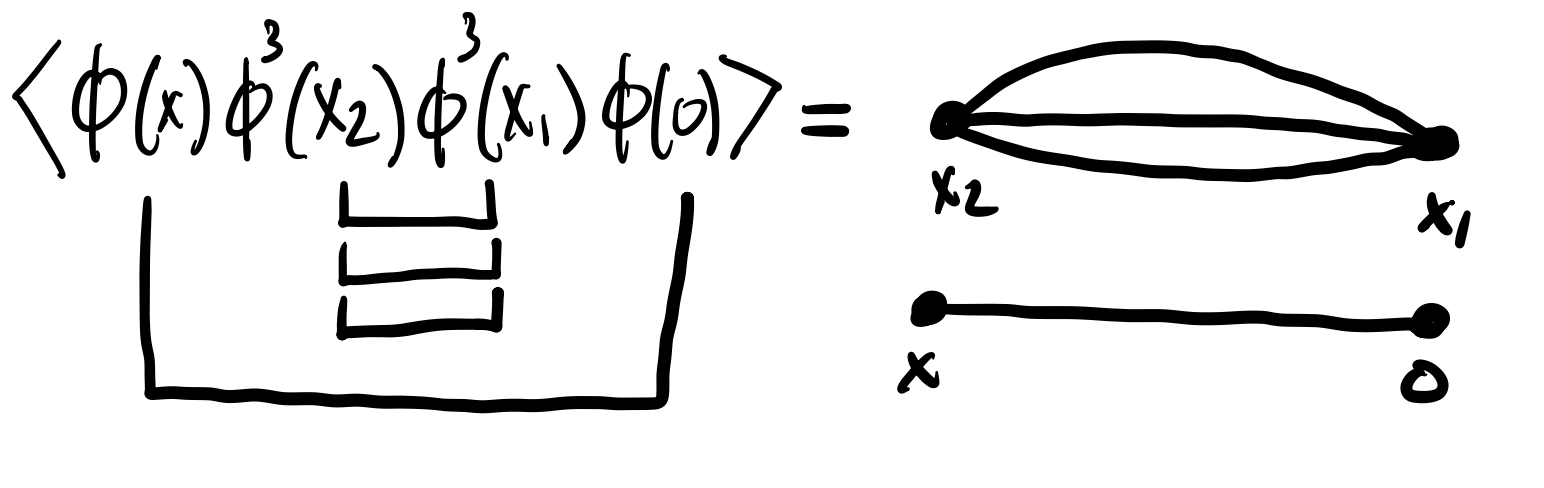
\includegraphics[scale=0.4]{Lectures/Figures/lec11-diag1.png}
\end{center}

The only other option is where we contract two $\phi(x_2)$s together, contract two $\phi(x_1)$, and finally contract one $\phi(x_1)$ with $\phi(x_2)$, which gives:

\begin{equation}
    G(x)G(0)^2G(x_2 - x_1)
\end{equation}

\begin{center}
    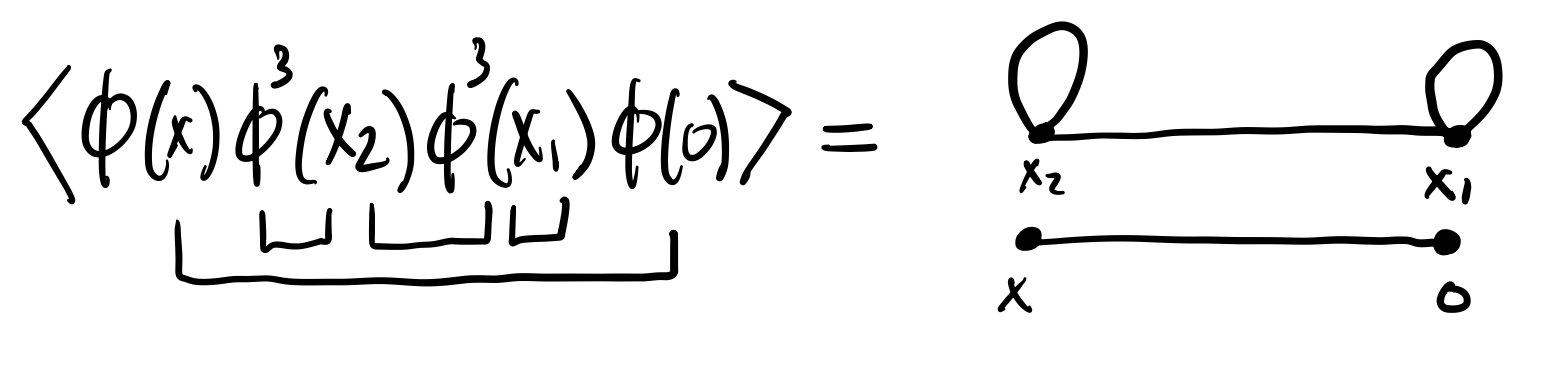
\includegraphics[scale=0.4]{Lectures/Figures/lec11-diag2.png}
\end{center}

These are a special type of diagram, because if we look at the $\avg{\phi(x)\phi(0)}_0\avg{S_{\text{int}}^2}_0$ term we will see they get exactly cancel. These diagrams are sometimes called ``bubble diagrams'' because there are bubbles/parts of the diagram that are separate from the main propagator (i.e. diagrams of the form $G(x) \cdot (\text{stuff})$\footnote{Luca - ``This is the formal definition.''}). Although we saw a specific example here, it is in fact generally true that they get cancelled from $\frac{1}{\int \mathcal{D} \phi e^{iS}}$.

What we are left with is:
\begin{equation}
    \avg{\phi(x)\phi(0)}_\lambda = \avg{\phi(x)\phi(0)}_0 + \frac{i^2}{2}\left.\avg{\phi(x)S^2_{\text{int}}\phi(0)}\right|_{\text{non-bubble}}
\end{equation}
Which contractions are left? Qualitatively, three. The first is where we contract $\phi(x)$ with a $\phi(x_2)$, $\phi(0)$ with a $\phi(x_1)$, and then pair up the remaining $\phi(x_2)$s with $\phi(x_1)$s, which gives:
\begin{equation}
    G(x - x_2)G(x_2 - x_1)^2 G(x_1)
\end{equation}
\begin{center}
    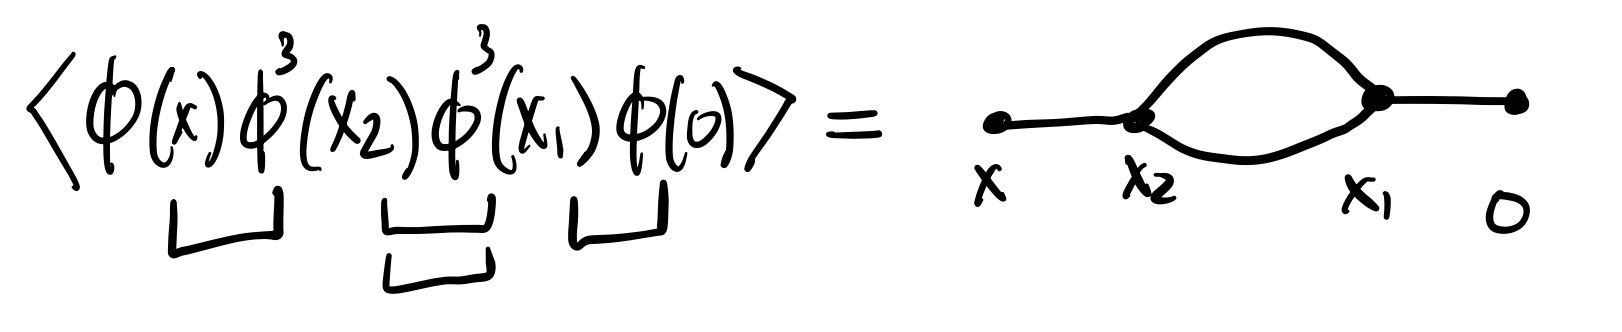
\includegraphics[scale=0.4]{Lectures/Figures/lec11-diag3.png}
\end{center}
The second is where we contract $\phi(x)$ with $\phi(x_2)$, and $\phi(0)$ is also contracted with $\phi(x_2)$. Then, we contract the remaining $\phi(x_2)$ with one $\phi(x_1)$ and two $\phi(x_1)$s together. This gives:
\begin{equation}
    G(x - x_2)G(x_2 - x_1)G(0)G(x_2)
\end{equation}
\begin{center}
    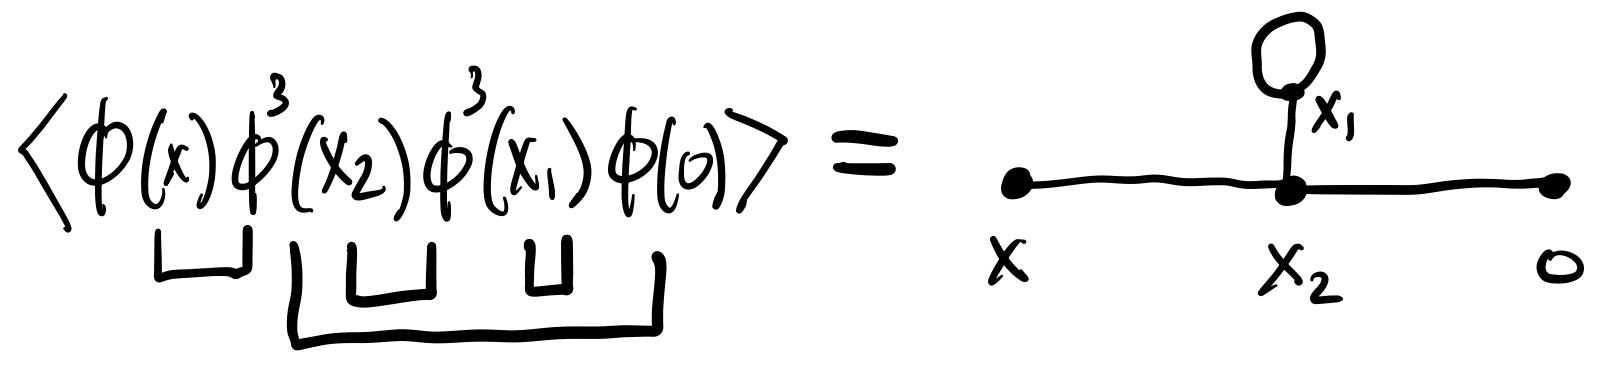
\includegraphics[scale=0.4]{Lectures/Figures/lec11-diag4.png}
\end{center}
Finally, in the last contraction we keep the left and right halves separate; contract $\phi(x)$ with a $\phi(x_2)$, $\phi(0)$ with $\phi(x_1)$, and $\phi(x_2)$s together and $\phi(x_1)$s together. This gives:
\begin{equation}
    G(x - x_2)G(0)^2 G(x_1)
\end{equation}
\begin{center}
    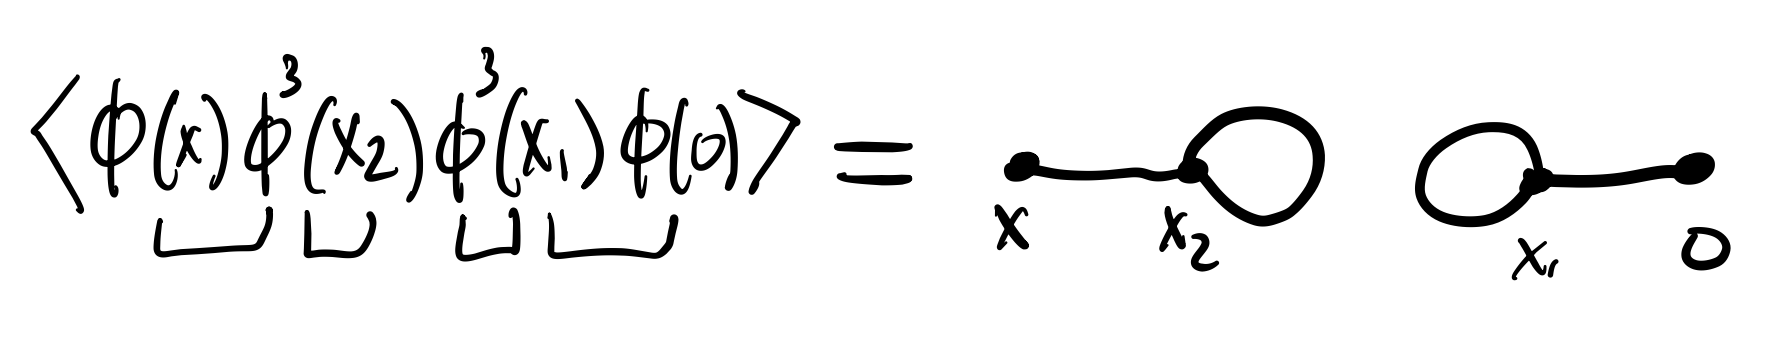
\includegraphics[scale=0.4]{Lectures/Figures/lec11-diag5.png}
\end{center}

Out of these diagrams, the last one is special. It is disconnected, i.e. there is no connection between $x$ and $0$, thus it does not depend on the distance between $x$ and $0$. It will get cancelled out when we look at the connected correlation function, as these diagrams are precisely the corrections to the one-point functions, i.e. $\avg{\phi(x)}\avg{\phi(0)}$, where the correction to $\avg{\phi(x)}$ corresponds to the left piece of the above diagram and $\avg{\phi(0)}$ corresponds to the right piece of the above diagram.

The final result is that:
\begin{equation}
    \avg{\phi(x)\phi(0)}_{\lambda, c} = \avg{\phi(x)\phi(0)}_0 + \frac{i^2}{2}\left.\avg{\phi(x)(S_{\text{int}})^2\phi(0)}\right|_{\text{no bubbles, connected}} + O(\lambda^3)
\end{equation}
and we will go through this on Thursday in more detail, getting the combinatorial factors right.
\newpage
\section{Our First Interacting Theory Part II}
Last class, we looked at our first interacting QFT - we looked at an interaction term in the action, $S_{\text{int}} = -\frac{\lambda}{(3!)^2}\int d^D x \phi^3$. We worked perturbatively in the interaction, and found that we could find correlation functions in the interacting theory in terms of (harder, but computable) correlation functions in the free theory. We found that, if we look at the connected correlation functions:
\begin{equation}
    \avg{\phi(x)\phi(0)}_{\lambda, c} = \avg{\phi(x)\phi(0)} + \frac{i^2}{2}\left.\avg{\phi(x)S_{\text{int}}^2\phi(0)}\right|_{\text{no bubbles, connected}} + O(\lambda^3)
\end{equation}
i.e. that with connected correlators, disconnected and bubble diagrams had no contributions. This is in fact general. Connected correlators, which generically are defined as:
\begin{equation}
    \fd{^n}{(iJ)^n}\log Z[J]
\end{equation}
only receive contributions from connected Feynman diagrams.

\subsection{Symmetry Factors}
The two remaining diagrams that contributed ended up being diagram (A):
\begin{equation}
    G(x - x_2)G(x_2 - x_1)^2 G(x_1)
\end{equation}
\begin{center}
    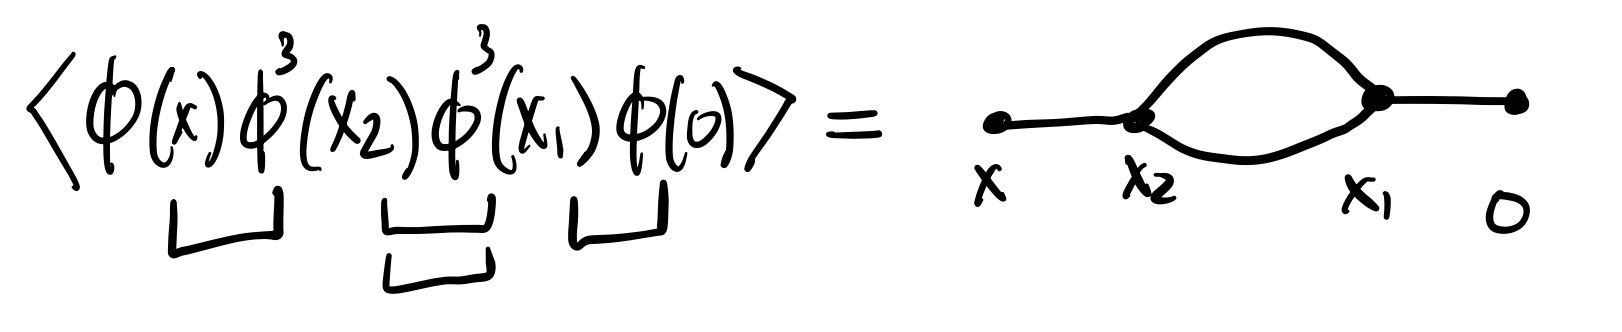
\includegraphics[scale=0.4]{Lectures/Figures/lec11-diag3.png}
\end{center}
and diagram (B):
\begin{equation}
    G(x - x_2)G(x_2 - x_1)G(0)G(x_2)
\end{equation}
\begin{center}
    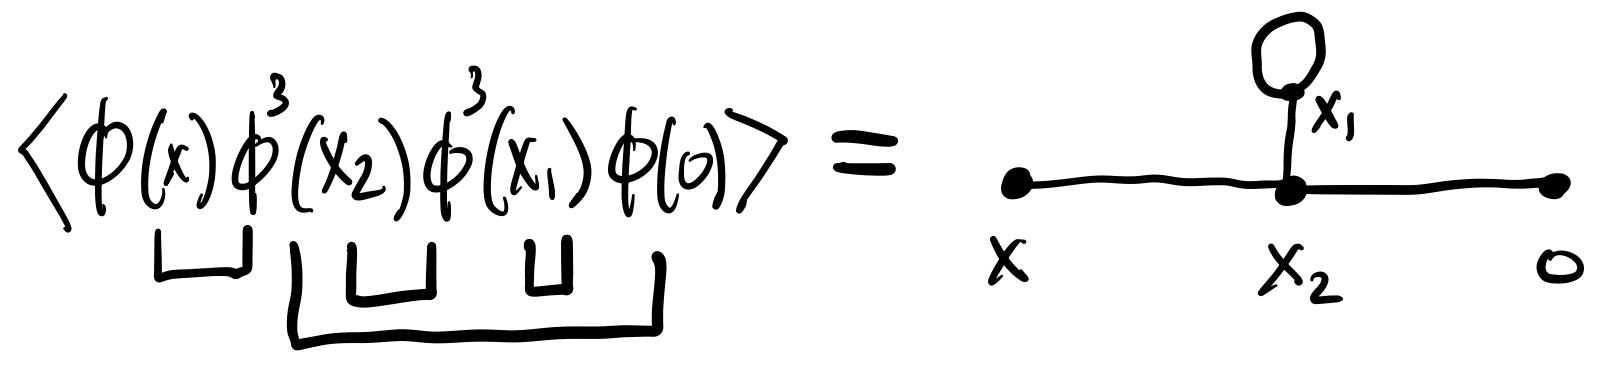
\includegraphics[scale=0.4]{Lectures/Figures/lec11-diag4.png}
\end{center}
which we will look at in more detail today. We'll study diagram (A), and we'll leave B for the problem set.

The contribution from all contractions is:
\begin{equation}
    \frac{i^2}{2}\frac{\lambda^2}{(3!)^2}\int_{x_1, x_2}\left.\avg{\phi(x)\phi^3(x_2)\phi^3(x_1)\phi(0)}_0\right|_{\text{no bubbles, connected}}
\end{equation}
We note that there are several Wick contractions that lead to the same diagram. All choices give the same diagram, but we need to take into account the symmetry factor of the diagram (how many choices of contractions). Let's think about the symmetry factor for (A). 
\begin{itemize}
    \item First, we want to contract $\phi(x)$ with fields at $x_1$ or at $x_2$. This gives us a factor of 2.
    \item Further, after choosing one of $x_1$ or $x_2$, we have a choice of three fields to contract with (as we have $\phi(x_1)^3/\phi(x_2)^3$). This gives a factor of 3.
    \item Now, for diagram A, $\phi(0)$ must be contracted with the remaining one of $x_1/x_2$. There are then 3 possible fields for it to be contracted with, giving a factor of 3.
    \item We have two remaining fields each in $\phi(x_1), \phi(x_2)$. We don't want to contract $\phi(x_1)$ with itself as that gives a disconnected diagram. So, there are two possible contractions between the two $\phi(x_1)$s and the two $\phi(x_2)$s. This gives a factor of 2.
\end{itemize}
In total, the symmetry factor of diagram (A) is:
\begin{equation}
    2 \cdot 3 \cdot 3 \cdot 2 = 36 = (3!)^2
\end{equation}
Which cancels out the $(3!)^2$ in the denominator, and so the A part of the correlator is:
\begin{equation}
    (A) =  -\frac{\lambda^2}{2}\int_{x_1, x_2}G(x - x_2)G(x_2 - x_1)^2 G(x_1)
\end{equation}

Physically, we can view this as the propogation in spacetime sketched below:

\begin{figure}[htbp]
    \centering
    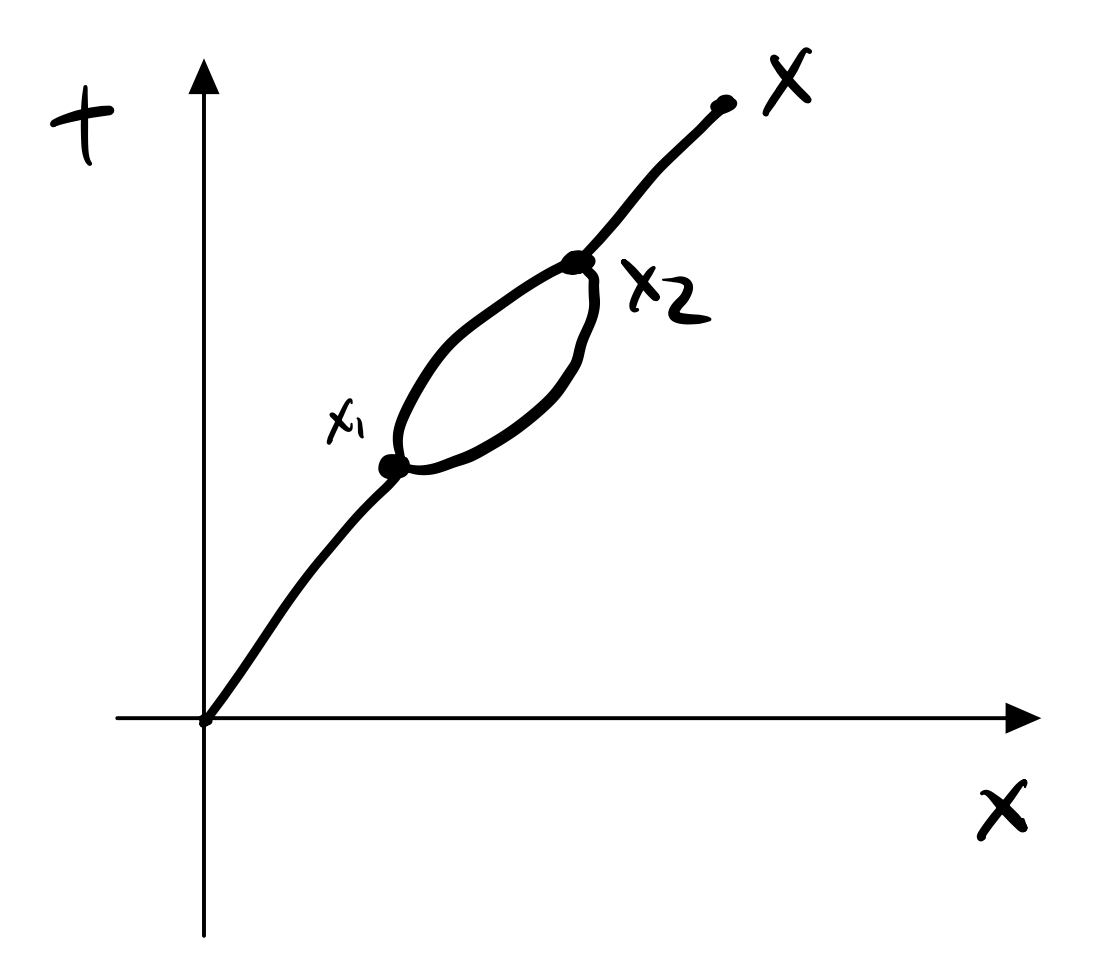
\includegraphics[scale=0.3]{Lectures/Figures/interactingprop-spacetime.png}
    \caption{Picture of the interacting diagram as a particle propagating in spacetime.}
    \label{fig:interactingprop-spacetime}
\end{figure}

It ``looks like'' the particle splits into two at $x_1$ due to the interaction, and then recombines at $x_2$. Compare this to the free theory, where the particle just propagates from $0$ to $x$.

\subsection{Going to Momentum Space}
We have nice expressions for these Green's functions in momentum space:
\begin{equation}
    G(x_1) = \int \frac{d^Dp_1}{(2\pi)^D}e^{ip_\mu x^\mu_1}G(p_1) = \int \frac{d^Dp_1}{(2\pi)^D}e^{ip_\mu x^\mu_1} \frac{-i}{p_1^2 + m^2 - i\e}
\end{equation}
So Fourier transforming each of the Green's functions in the (A) expression:
\begin{equation}
    (A) = -\frac{\lambda^2}{2}\int d^{D}x_1 d^D x_2\int \frac{d^Dp_1d^Dp_2d^Dp_3d^Dp_4 }{(2\pi)^{4D}} e^{ip_4(x - x_2)}e^{ip_3(x_2- x_1)}e^{ip_2(x_2 - x_1)}e^{ip_1(x_1)}G(p_4)G(p_3)G(p_2)G(p_1)
\end{equation}
The $x_1$ integral gives:
\begin{equation}
    (2\pi)^D \delta^D(p_1 - p_2 - p_3) \implies p_3 = p_1 - p_2
\end{equation}
and the $x_2$ integral gives:
\begin{equation}
    (2\pi)^d \delta^D(p_4 - p_2 - p_3) \implies p_4 = p_2 + p_3 = p_1
\end{equation}
We are thus left with:
\begin{equation}
    (A) = -\frac{\lambda^2}{2}\int_{p_1p_2}e^{ip_1 x}G(p_1)G(p_2)G(p_1 - p_2)G(p_1) = \delta G(x)
\end{equation}
Fianlly, Fourier transforming the result:
\begin{equation}
    \delta G(p) = \int d^Dx e^{-ipx}\delta G(x)
\end{equation}
which gives a factor of $(2\pi)^D \delta(p_1 - p)$, we obtain:
\begin{equation}
    \delta G(p) = -\frac{\lambda^2}{2}\int \frac{d^Dp_2}{(2\pi)^D}G(p)G(p_2)G(p - p_2)G(p) = -\frac{\lambda^2}{2}G(p)^2\int \frac{d^Dp'}{(2\pi)^D}G(p')G(p -p')
\end{equation}
This expression suggests a momentum space interpretation of the Feynman rules. A particle comes in with momentum $p$, then splits into to particles with momenta $p'$ and $p - p'$ (such that the momentum is conserved at the vertex), recombining into a particle with momentum $p$ at the end of the loop. The loop momentum $p'$ is integrated over. More consisely, we can say that the ``momentum space Feynman rules'' are:
\begin{itemize}
    \item Momentum are conserved at vertices of momentum space Feynman diagrams.
    \item Loop momentum are integrated over.
\end{itemize}
Instead of learning a bunch of Feynman rules/diagrams by heart (as might be the older approach to QFT), it's better to know how to derive them using the path integral, as there are many interesting known QFTs!

\begin{figure}[htbp]
    \centering
    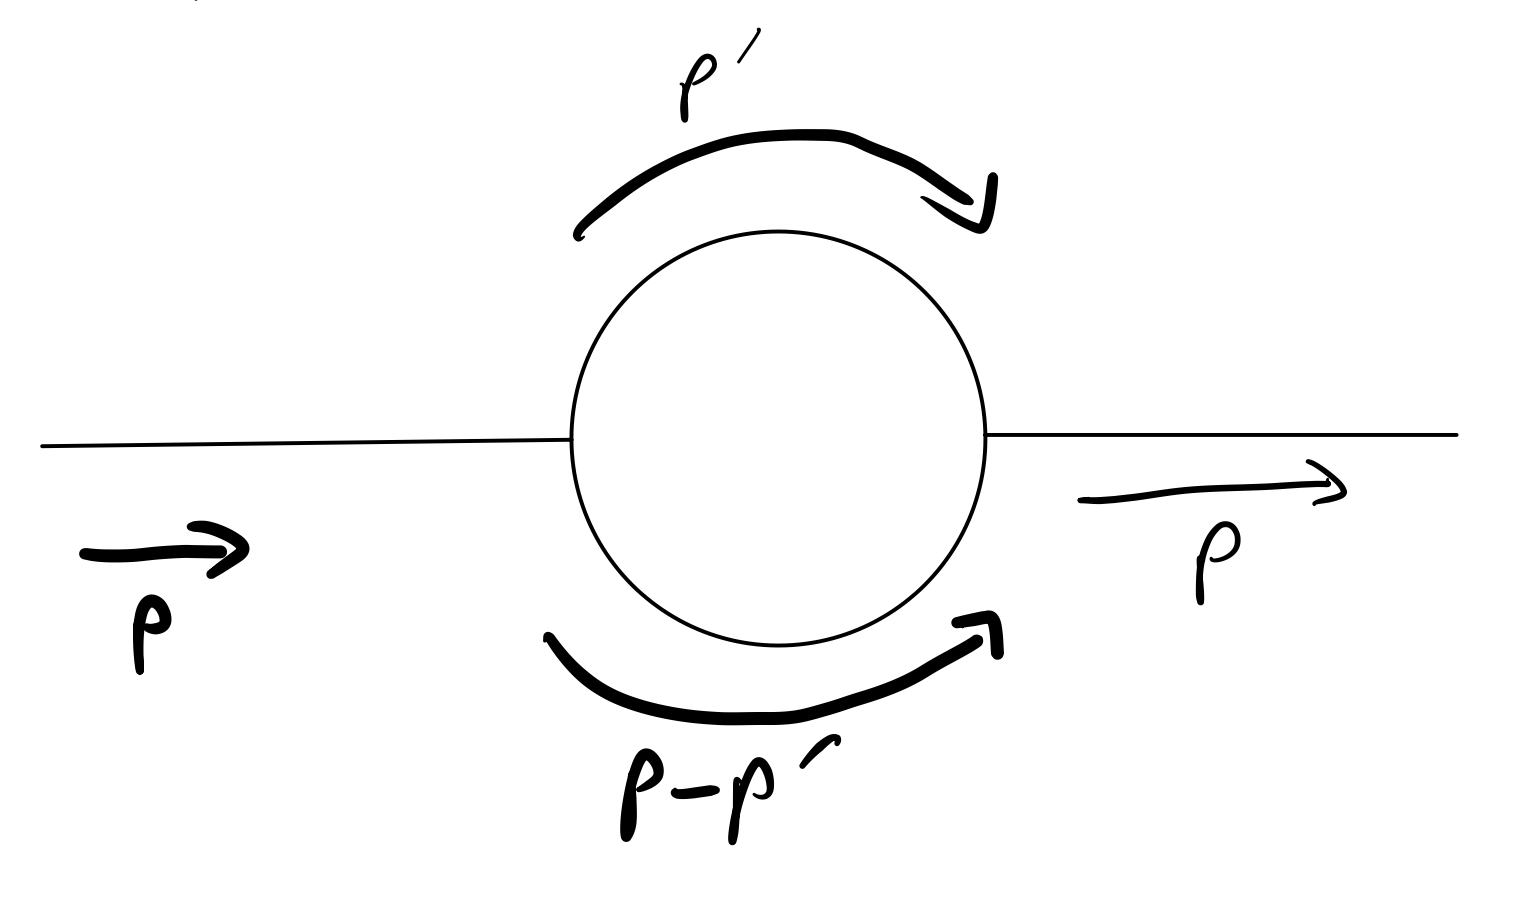
\includegraphics[scale=0.3]{Lectures/Figures/interactingprop-momentum.png}
    \caption{Picture of the interacting diagram as a particle propagating in momentum space.}
    \label{fig:interactingprop-momentum}
\end{figure}

\subsection{Self-Energy and Computing the Loop Integral}
Before trying to compute this integral, there is a useful parameterization of this correction in terms of a (small) ``self-energy\footnote{not a particularly great name}'' $\Pi$. In terms of this, we can write the interacting Green's function as:
\begin{equation}
    G_{\text{int}}(p) = G(p) + \delta G(p) = \frac{-i}{p^2 + m^2 + \Pi(p)} = \frac{-i}{p^2 + m^2}\frac{1}{1 - \frac{\Pi(p)}{p^2 + m^2}} \approx \frac{-i}{p^2 + m^2}\left(1 + \frac{\Pi(p)}{p^2 + m^2} + \ldots \right)
\end{equation}
at this point we aren't justified in keeping the higher order terms, because we've only worked to $O(\lambda^2)$ and the higher order terms are in higher powers of $\lambda$. But, to linear order in the self energy (which is $O(\lambda^2)$):
\begin{equation}
    G_{\text{int}}(p) = G(p) + G(p)^2 i\Pi(p)
\end{equation}
i.e. we have re-packaged the correction in terms of $\Pi(p)$. So:
\begin{equation}
    \Pi(p) = \frac{i\lambda^2}{2}\int \frac{d^Dp'}{(2\pi)^D}G(p')G(p - p')
\end{equation}
Which can be viewed as just the loop part of the momentum-space Feynman diagram. We know the free Feynman propagators, and so can write the above as:
\begin{equation}
    \Pi(p) = \frac{i\lambda^2}{2}\int \frac{d^Dp'}{(2\pi)^D}\frac{-i}{p'^2 + m^2 - i\e}\frac{-i}{(p - p')^2 + m^2 - i\e}
\end{equation}
The computation is technical, but it will be our first concrete/worked out result in interacting QFT, so it wil be worth it.

We consider the following recipe for evaluating loop integrals:
\begin{itemize}
    \item If the integrals involve more than one propagator (in our case, 2), we can use Feynman parameters to simplify down into one denominator.
    \item The $i\e$ appearing in the denominators can be slightly hard to work with. We will ``Wick rotate'', i.e. perform a contour deformation in the frequency $p_0'$. This integral has poles at (roughly) $p_0' = \pm \sqrt{\v{p}'^2 + m^2 - i\e}$. If we Taylor expand the $i\e$, the poles are at $p_0' = \pm \sqrt{\v{p}'^2 + m^2} \mp i\e$. If we look at this in the complex plane, we can consider the contour:
    
    \begin{figure}[htbp]
        \centering
        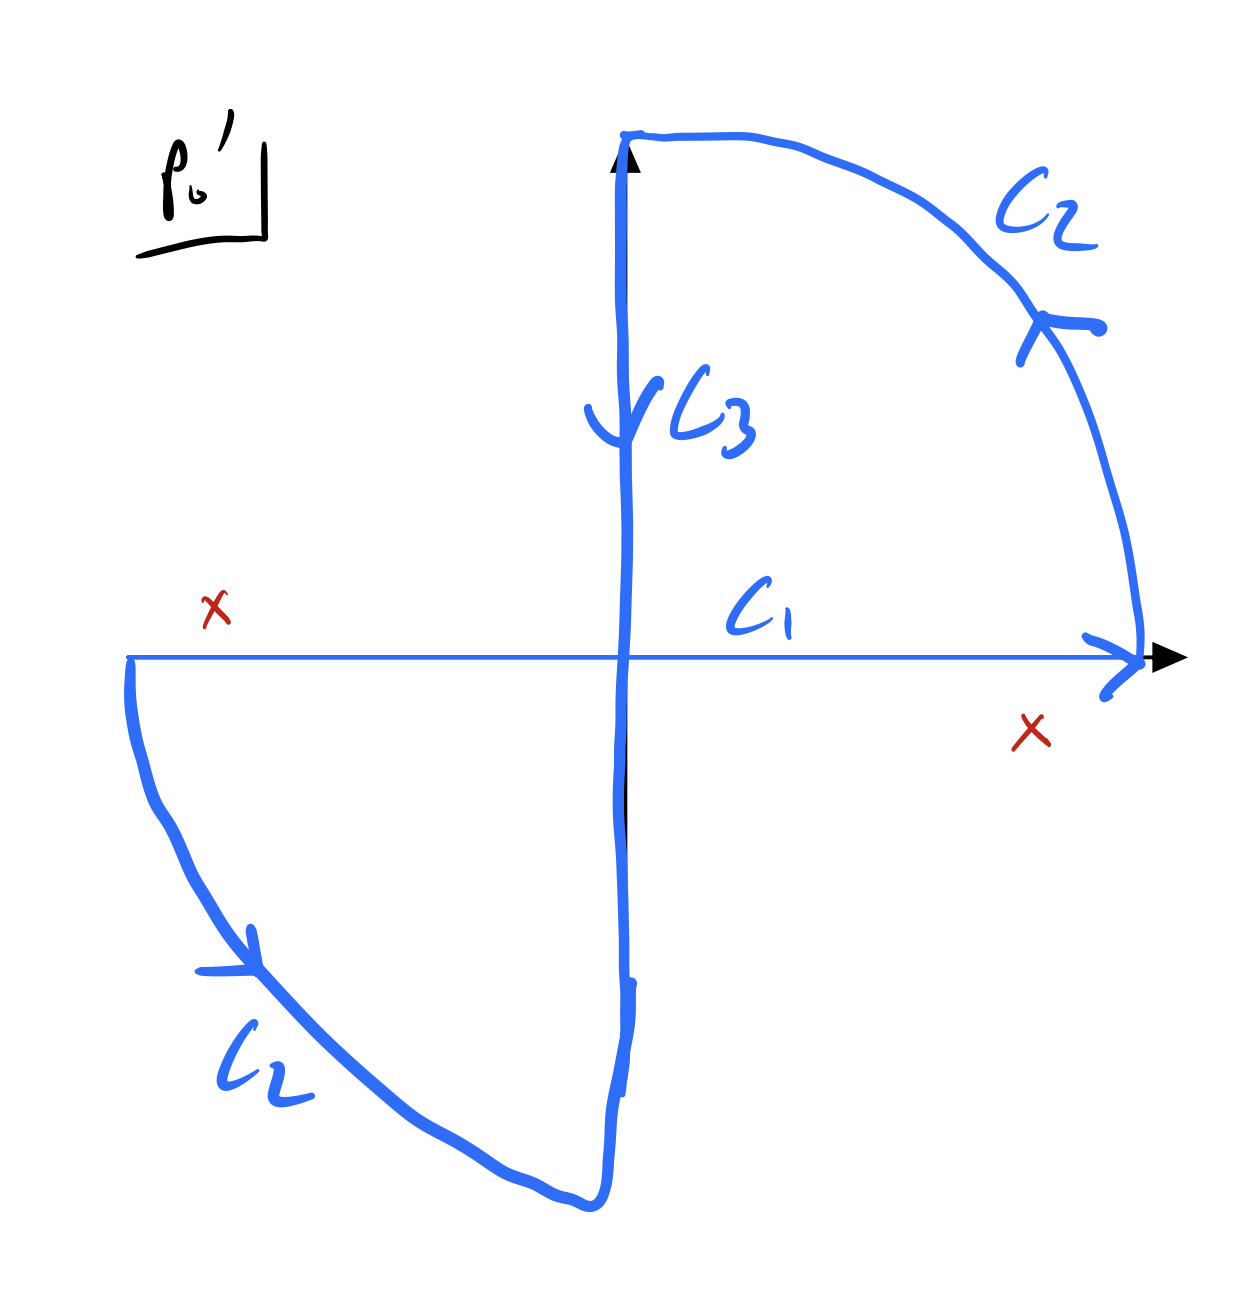
\includegraphics[scale=0.3]{Lectures/Figures/butterflycontour.png}
        \caption{Contour integral of $p_0'$ in $\CC^2$, which will allow us to write the desired integral (along the real axis) in terms of a ``Wick rotated'' integral along the imaginary axis.}
        \label{fig:butterflycontour}
    \end{figure}

    Then, we find that (since the contour contains no poles):
    \begin{equation}
        \int_{C_1 \cup C_2 \cup C_3} dp_0' (\ldots) = 0
    \end{equation}
    Thus, rephrasing this in terms of the integral that we want, i.e. that over $C_1$:
    \begin{equation}
        \Pi(p) = \int_{C_1}p_0' (\ldots)  = -\int_{C_2} dp_0'(\ldots) - \int_{C_3} dp_0'(\ldots).
    \end{equation}
    as we send the $C_2$ contour to infinity, it will vanish, and so:
    \begin{equation}
        \Pi(p) = -\int_{C_3} dp_0'(\ldots) = \int_{+i\infty}^{-i\infty}dp_0' (\ldots)
    \end{equation}
    Along this whole contour, $p_0'$ is imaginary, so let us do the change of variable $p_0' = ip_0'^E$:
    \begin{equation}
        \Pi(p) = i\int_{-\infty}^\infty dp_0'^E (\ldots)
    \end{equation}
    so far it seems like we've made the problem no better, no worse. Just integrating along a different axis. But - the resulting integral will turn out to be much nicer! This is because:
    \begin{equation}
        p'^2 = p_\mu' p'^\mu = -p_0'^2 + p_i'^2 = (p_0'^E)^2 + p_i'^2 = p_E^2
    \end{equation}
    which is just the Euclidean norm in $D$ dimensions! I.e. we are working in regular space, not Minkowski (where the $-$ sign on the time component can make our lives a bit more complicated).
\end{itemize}

Alright, we've laid out the steps, let's go through the integral! we want to compute:
\begin{equation}
    \Pi(p) = \frac{i\lambda^2}{2}\int \frac{d^Dp'}{(2\pi)^D}\frac{-i}{p'^2 + m^2 - i\e}\frac{-i}{(p - p')^2 + m^2 - i\e}
\end{equation}
We do a trick to put this over a single denominator. We use the fact that:
\begin{equation}
    \begin{split}
        \int_0^1 dx \frac{1}{[xA + (1-x)B]^2} = \int_0^1 dx \frac{1}{(x(A - B) + B)^2} &=\left.-\frac{1}{(A-B)}\frac{1}{x(A - B) + B}\right|_0^1 
        \\ &= \frac{1}{A-B}\left(\frac{1}{B} - \frac{1}{A}\right) = \frac{1}{A-B}\frac{A-B}{A+B} = \frac{1}{AB}
    \end{split}
\end{equation}
Thus, applying this identity to the above, with:
\begin{equation}
    \begin{split}
        A &= (p' - p)^2 + m^2 - i\e
        \\ B &= p'^2 + m^2 - i\e
    \end{split}
\end{equation}
We obtain:
\begin{equation}
    \Pi(p) = -\frac{i\lambda^2}{2}\int_0^1 dx\int_{p'}\frac{1}{(x[(p' - p)^2 + m^2 - i\e] + (1-x)[p'^2 + m^2 - i\e])^2}
\end{equation}
Simplifying the denominator:
\begin{equation}
    \begin{split}
        \Pi(p) &= -\frac{i\lambda^2}{2}\int_0^1 dx\int_{p'} \frac{1}{[m^2 - i\e + p'^2 - 2p\cdot p'x + p^2x]^2} 
        \\ &= -\frac{i\lambda^2}{2}\int_{p'} \frac{1}{[(p' - xp)^2 + m^2 + p^2x(1-x) - i\e]^2}
        \\ &= -\frac{i\lambda^2}{2}\int_0^1 dx \int_q \frac{1}{(q^2 + \Delta - i\e)^2}
    \end{split}
\end{equation}
where in the second equality we complete the square and in the third equality we introduce a new variable of integration $q = p' - xp$ and define $\Delta = m^2 + p^2x(1-x)$ which does not depend on $q$. Now, this integral has a simple pair of poles, and we should be able to use the Wick rotation trick. Let us do it; substitute $q_0 \to iq_0^E$, so:
\begin{equation}
    \Pi(p) = \frac{\lambda^2}{2}\int_0^1 dx \int \frac{d^Dq_E}{(2\pi)^D} \frac{1}{(q_E^2 + \Delta - i\e)^2}
\end{equation}
where $q_E^2 = (q_E^0)^2 + (q_E^i)^2$ is the regular Euclidean norm. Let us go into spherical coordinates to evaluate this, as we observe that there is nothing in the integral that depends on the angles, only the magnitude of $q_E$:
\begin{equation}
    \Pi(p) = \frac{\lambda^2}{2} \int_0^1 dx \int \frac{dq_E q_E^{D-1}d^{D-1}\Omega}{(2\pi)^D}\frac{1}{(q_E^2 + \Delta - i\e)^2} = \frac{\lambda^2}{2} \frac{S_{D-1}}{(2\pi)^D}\int_0^1 dx \int_0^\infty q_E^{D-1}\frac{1}{(q_E^2 + \Delta - i\e)^2}
\end{equation}
where $S_{D-1}$ is the surface area of the unit $n$-sphere, i.e. $S_1 = 2\pi$, $S_2 = 4\pi$, $S_3 = 2\pi^2$. We can further simplify because the $\e$ is no longer relevant, it just was there to tell us how to Wick-rotate. Thus:
\begin{equation}
    \Pi(p) = \frac{\lambda^2}{2}\frac{S_{D-1}}{(2\pi)^D}\int_0^1 dx \int_0^\infty \frac{dq_E q_E^{D_1}}{(q_E^2 + \Delta)^2}
\end{equation}
So just 2 more integrals to go!

BUT now tragedy strikes. This integral actually diverges for $D \geq 4$ (for $D = 4$, we can see that it goes as $\log(q_E)$, and powers of $q_E$ for $D >4$). This is what is known as an ultraviolet divergence\footnote{Be thankful that you live in the 21st century, where we understand these completely!} To resolve this, let us introduce a sharp ultraviolet cutoff $\Lambda$:
\begin{equation}
    \int_0^{\infty} dq_E \to \int_0^\Lambda dq_E
\end{equation}
Then we obtain (in $D = 4$):
\begin{equation}
    \Pi(p) = \frac{\lambda^2}{2}\frac{2\pi^2}{(2\pi)^4}\int_0^1 dx \int_0^\Lambda dq_E \frac{q_E^2}{(q_E^2 + \Delta)^2}q_E
\end{equation}
Then we find:
\begin{equation}
    \int_0^\Lambda dq_E \frac{q_E^2}{(q_E^2 + \Delta)^2}q_E = \left. \frac{1}{2}\left(\frac{\Lambda}{q_E^2 + \Delta} + \log(q_E^2 + \Delta)\right)\right|_{0}^\Lambda = \frac{1}{2}\left(\log(\Lambda^2 + \Delta) + \frac{\Delta}{\Lambda^2 + \Delta} - \frac{1}{2}(1 + \log \Delta)\right)
\end{equation}
So, keeping in mind that $\Lambda$ is very large and keeping only the dominant terms in $\Lambda$, i.e.:
\begin{equation}
    \log(\Lambda^2 + \Delta) + \frac{\Delta}{\Lambda^2 + \Delta} \approx \log\Lambda^2 + O(\frac{\Delta}{\Lambda^2})
\end{equation}
we find:
\begin{equation}
    \Pi(p) = \frac{\lambda^2}{(4\pi)^2}\int_0^1 dx \left(\frac{1}{2}\log\Lambda^2 - \frac{1}{2} - \frac{1}{2}\log\Delta\right).
\end{equation}
Let's focus on the UV divergent $\log \Lambda$ piece:
\begin{equation}
    \left.\Pi(p)\right|_{\text{div}} = \frac{\lambda^2}{(4\pi)^2}\int_0^1 dx \log\Lambda = \frac{\lambda^2}{(4\pi)^2}\log \Lambda
\end{equation}
recall that:
\begin{equation}
    G_{\text{int}}(p) = \frac{-i}{p^2 + m^2 - \Pi(p)} = \frac{-i}{p^2 + m^2 - \lambda^2\frac{\log \Lambda}{(4\pi)^2}}
\end{equation}
this corresponds to a (momentum-independent) shift in the mass term. In the interacting theory, the physical pole is no longer simply given by the bare mass. The physical mass that the experimentalist measures now appears to be regulator-dependent:
\begin{equation}
    m_{\text{phys}}^2 = m^2 -\lambda^2\frac{\log \Lambda}{(4\pi)^2}
\end{equation}
This might sound upsetting, and Luca is going to leave this to sit with us for the weekend. But, next week we will resolve it, beautifully!
\newpage
\section{Counterterms and Non-Analytic Contributions}
\subsection{Review}
We were studying the interacting scalar field theory:
\begin{equation}
    S = -\int d^Dx \frac{1}{2}(\p\phi)^2 + \frac{1}{2}m^2\phi^2 + \frac{1}{3!}\lambda \phi^3
\end{equation}
We found that the 2-point function receives a $O(\lambda^2)$ correction:
\begin{equation}
    \avg{\phi(x)\phi(0)}_C = \avg{\phi(x)\phi(0)}_0 + \frac{i^2}{2}\left.\avg{\phi(x)S_{\text{int}}^2 \phi(0)}_0\right|_{\text{connected diagram}} + O(\lambda^4)
\end{equation}
where we note that there is no $\lambda^3$ correction as the free theory has a $\mathbb{Z}_2$ symmetry. In momentum space:
\begin{equation}
    G_{\text{int}}(p) = G(p) + \delta G(p)_{(A)} + \delta G(p)_{(B)} + \ldots = \frac{-i}{p^2 + m^2- \Pi(p)}
\end{equation}
which in terms of Feynman space Feynman diagrams:

\begin{center}
    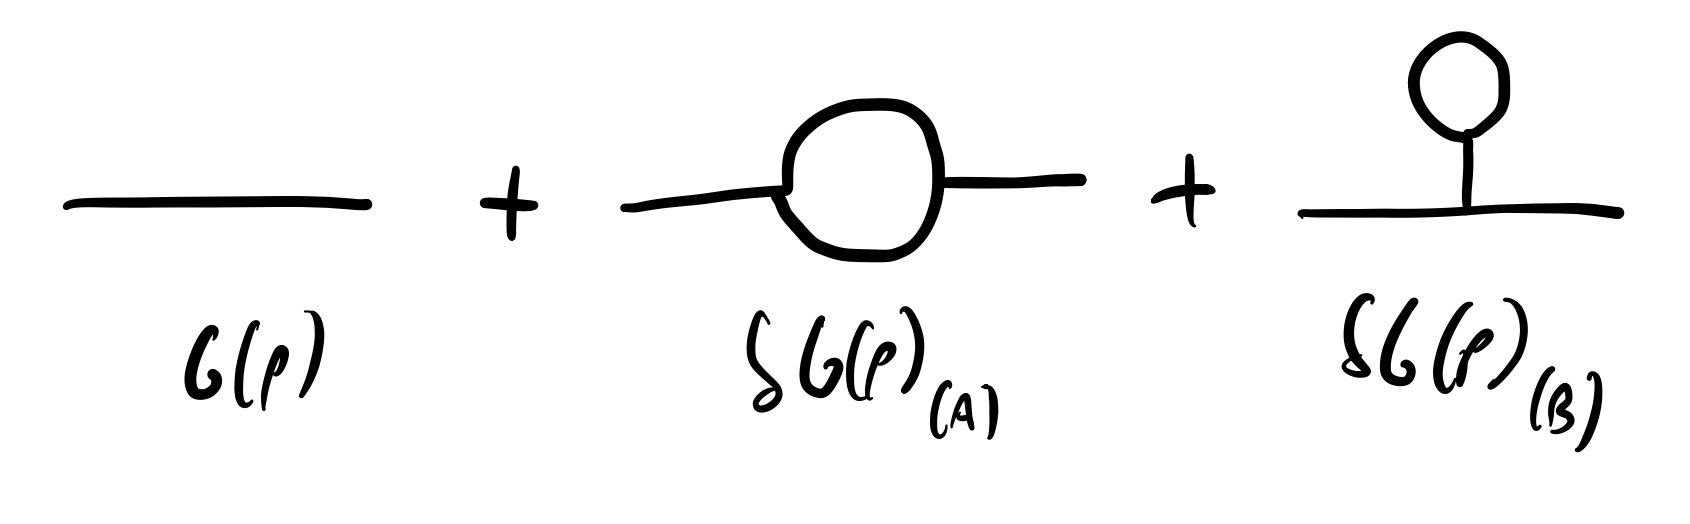
\includegraphics[scale=0.3]{Lectures/Figures/lec13-threediagrams.png}
\end{center}

The self-energy $\Pi(p)$ has two contributions, from the (A) diagram and the (B) diagram. The (A) diagram has contribution (the $(B)$ diagram contribution you study in PS6):
\begin{equation}
    \Pi_{(A)}(p) = \frac{i}{2}\lambda^2\int \frac{d^Dp'}{(2\pi)^D}G(p')G(p - p')
\end{equation}
Note that the (A) diagram gives non-analytic contributions, which is what gives the theory some predictive power. The (B) diagram only has an analytic contribution. Diagramatically, the (A) self-energy looks like the truncated version of the (A) Green's function correction:

\begin{center}
    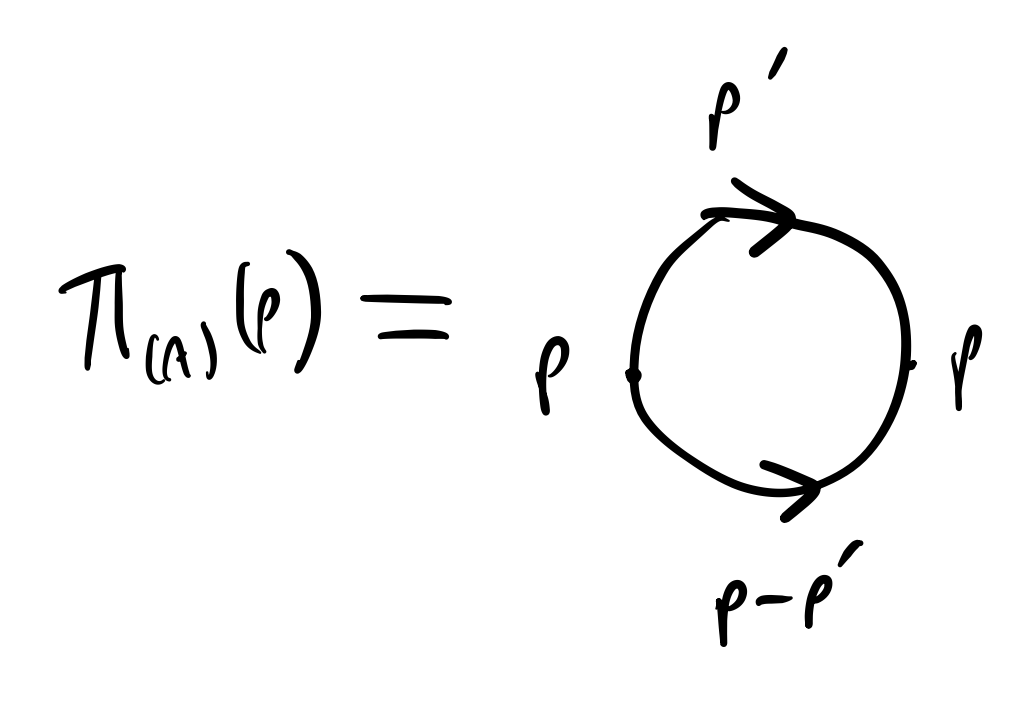
\includegraphics[scale=0.3]{Lectures/Figures/lec13-selfenergy.png}
\end{center}

We took steps towards computing the $\Pi_{(A)}$ integral. We introduced Feynman parameters to bring the two Green's functions over a single denominator, and then Wick rotated to convert the Minkowski product (with negative sign on the $0$th component of momentum) to the standard Euclidean product. Our result was spherically symmetric, and we we were left with:
\begin{equation}
    \Pi_{(A)}(p) = \frac{\lambda^2}{2}\frac{S_{D-1}}{(2\pi)^D}\int_0^1 dx \int_0^\infty dq_E \frac{q_E^{D-1}}{[q_E^2 + \Delta]^2}
\end{equation}
with $\Delta = m^2 +p^2x(1-x)$. This integral converges at $q_E = 0$, but as $q_E \infty$ the integrand goes as $\frac{q_E^{D-1}}{q_E^4} = q_E^{D-5}$ so as long as $D \geq 4$ the integral is UV divergent.

\subsection{Removing analytic divergences - counterterms}
So, we performed this integral with a regulator; a sharp momentum cutoff $\Lambda$. With this cutoff, we found (in $D = 4$):
\begin{equation}
   \int_0^\Lambda dq_E \frac{q_E^{3}}{(q_E^2 + \Delta)^2} = \frac{1}{2}\log \Lambda^2 - \frac{1}{2}\log \Delta(x, p^2) - \frac{1}{2} + O(\frac{1}{\Lambda^2})
\end{equation}
Thus:
\begin{equation}
    \Pi_{(A)}(p) = \frac{\lambda^2}{(4\pi)^2}\int_0^1 dx \frac{1}{2}\log \Lambda^2 - \frac{1}{2} - \frac{1}{2}\Delta(x, p^2) = \frac{\lambda^2}{(4\pi)^2}(\log\Lambda - \frac{1}{2}) - \frac{\lambda^2}{(4\pi)^2}\frac{1}{2}\int_0^1 dx \log\Delta(x, p^2)
\end{equation}
where the first term has no $p$-dependence and the second term has a non-analytic $p$-dependence. The full propagator is:
\begin{equation}
    G_{\text{int}}(p) = \frac{-i^2}{p^2+ m^2 - \Pi(p)}
\end{equation}
So; what we see is that the constant ($p$ independent) piece is just a shift of the mass. If $m$ is the bare mass that I had in the Lagrangian, this does not actually correspond to the pole of the propagator that is measured in the experiment. Further, its a UV divergent correction. But, crucially, this UV divergence can be removed by adding a local counterterm:
\begin{equation}
    \mathcal{L}_{ct} = -\frac{1}{2}\delta m^2 \phi^2
\end{equation}
with:
\begin{equation}
    \delta m^2 = \frac{\lambda^2}{(4\pi)^2}\log \Lambda
\end{equation}
then there is no divergence. So, if we sacrifice the simple relation between experimental parameters (the true mass) and the parameters in the Lagrangian, then we can remove the infinities, here. This tells us that we are not able to predict the mass/poles in this model. But, we can predict other things.

In PS6, you will set $D \geq 6$ and in this case, there are extra UV divergences. In $D = 6$ we see a subleading divergence in $p^2$:
\begin{equation}
    \Pi(p^2) = \lambda^2(c_1\Lambda^2 + c_2p^2\log\Lambda + \ldots)
\end{equation}
Because this divergence is analytic in momentum, we can remove it by adjusting derivative terms. The original Lagrangian had a $(\p\phi)^2$ term, but we can further add a $\frac{\delta Z}{2}(\p \phi)^2$ term to cancel it out. This is a very general approach to QFT, where divergences tell us about what cannot be predicted by the theory.

Perspectives on the UV cutoff; if not a HEP theorist, QFT is just an approximation to the system (an EFT), and in this case the cutoff is just a way of specifying where the EFT breaks down. Another perspective is that interacting QFTs are not defined with just an action; we need an action \emph{and} a regulator. 

\subsection{Renormalization Schemes}
One must choose - for bookkeeping - a ``renormalization scheme''.

For example, in the ``minimal subtraction'' scheme, one adds $\mathcal{L}_{ct}$ with $\delta m^2 = \frac{\lambda^2}{(4\pi)^2}\log \Lambda$. Doing this, the interacting Green's function will be:
\begin{equation}
    G_{\text{int}}(p) = \frac{-i}{p^2 + m_{\text{bare}}^2 + \text{finite}} \implies m_{\text{phys}}^2 = m_{\text{bare}}^2 + \text{finite}
\end{equation}
where the finite correction comes from the loop integral. Another perscription, which is what Srednicki uses, is to insist that the Lagrangian parameter $m_{\text{bare}}^2 = m_{\text{phys}}^2$; so, the counterterm is chosen to remove everything but this, i.e.:
\begin{equation}
    \delta m^2 = \frac{\lambda^2}{(4\pi)^2}\log \Lambda - \text{finite}
\end{equation}
so the pole is at $m_{\text{bare}}^2 = m_{\text{phys}}^2$. We all agree (experimentally) where the pole is, but the Lagrangian parameters may change. 

The bottom line - the relation between bare parameters and the true physical parameters is a subtle one.

\subsection{Non-analyticity and the continuum}
So far, this seems frustrating; we try to compute things in interacting QFTs, and all we learn is that the location of the pole is not something that we can predict. So now, let's talk about the good news, and talk about where interacting QFTs have predictive power. Let us study the non-analytic part of the self-energy:
\begin{equation}
    \Pi(p) = \text{analytic} - \frac{\lambda^2}{(4\pi)^2}\frac{1}{2}\int_0^1 dx \log \Delta(x, p^2), \quad \Delta = m^2 + p^2x(1-x)
\end{equation}
This piece is very interesting. Plugging it into mathematica, we have the result:
\begin{equation}
    \Pi(p) = \text{analytic} - \frac{\lambda^2}{(4\pi)^2}\frac{\text{arctanh}(\sqrt{\frac{p^2}{4m^2 + p^2}})}{\sqrt{\frac{p^2}{4m^2 + p^2}}}
\end{equation}
Where are the singularities of this integral? Let's explore its analytic structure. First, we have a denominator which could diverge. But, in fact this is not a singularity, because we have something of the form $\frac{\text{arctanh}(x)}{x}$, which is not actually singular as $x \to 0$ (due to the arctanh going to $0$ as well; in fact this function is analytic for $\abs{x} \leq 1$). So, $p \to 0$ is not a singularity. We do have singularities coming from the square roots, namely a branch point near $p^2= -4m^2$.

\begin{center}
    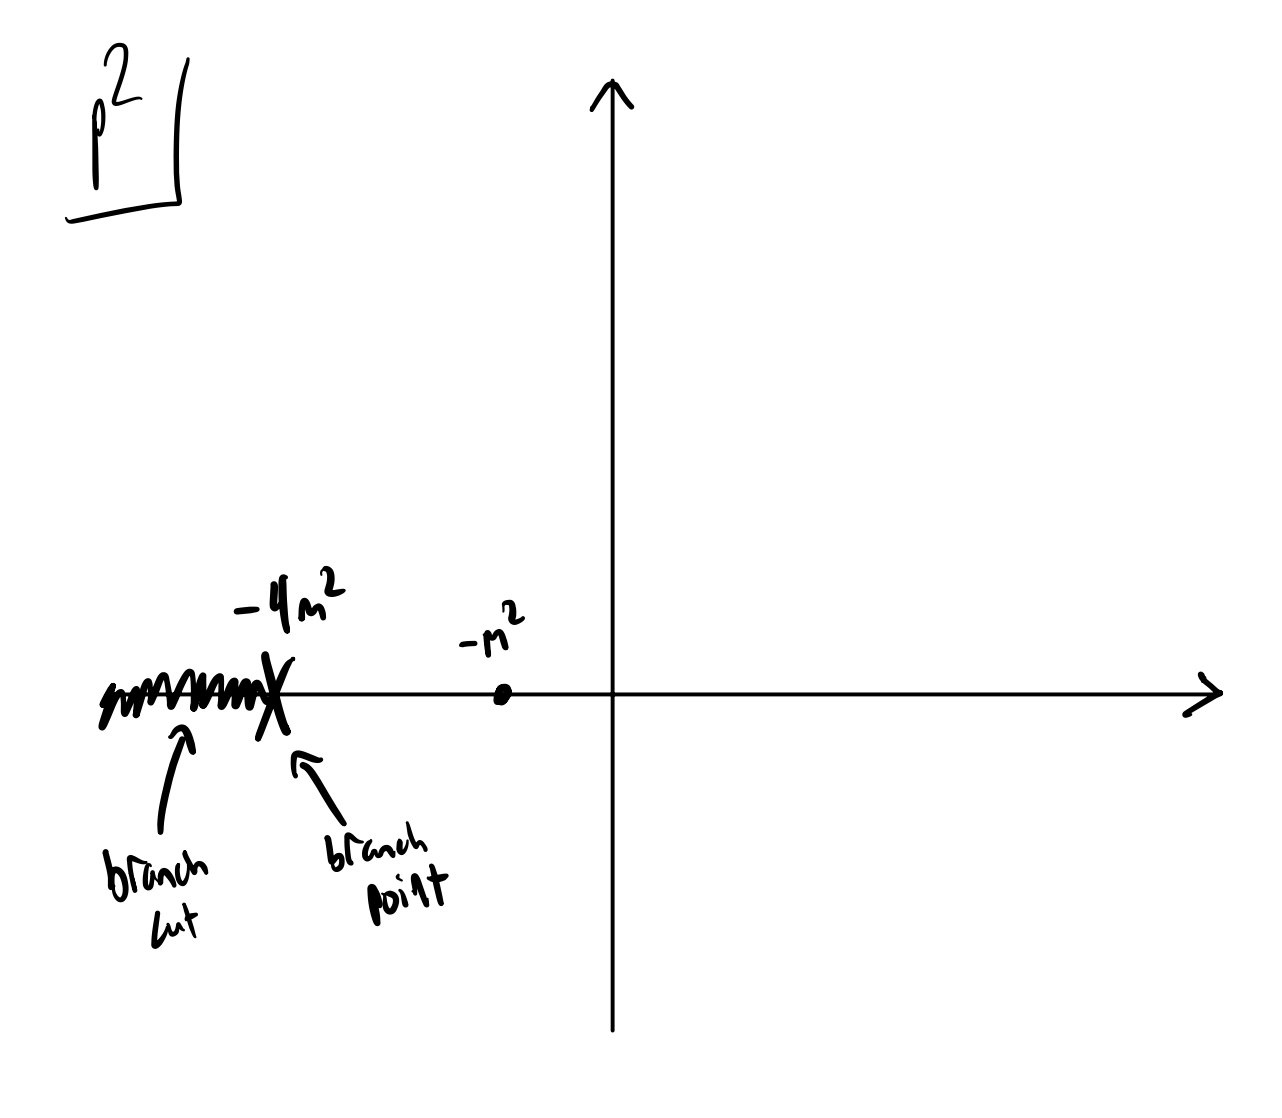
\includegraphics[scale=0.4]{Lectures/Figures/lec13-nonanalytic.png}
\end{center}

These non-analyticities are insensitives to UV divergences/counterterms. They tell us something very physical. Let's see what - it will be more intuitive to see what these are in terms of energy/frequency $p_0$. The non-analyticity is for:
\begin{equation}
    -p_0^2 + \v{p}^2 = p^2 \leq -4m^2 \implies p_0^2 \geq \v{p}^2 + 4m^2 \implies p_0 \geq \sqrt{\v{p}^2 + (2m)^2}
\end{equation}
Plotting this:

\begin{center}
    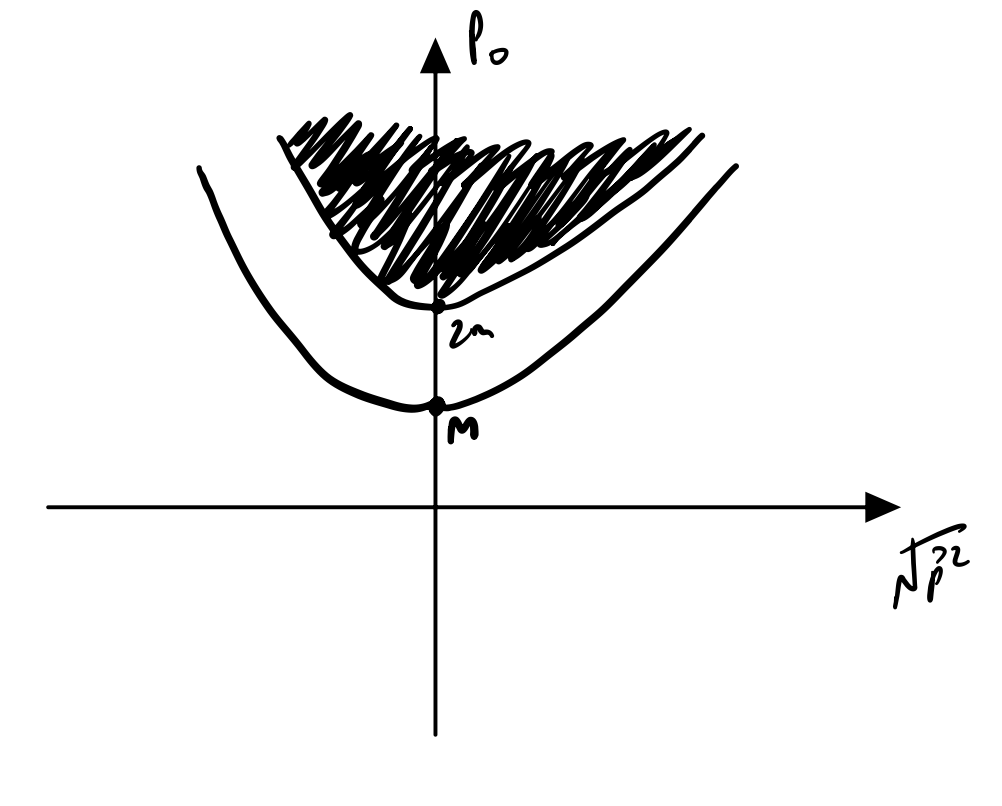
\includegraphics[scale=0.4]{Lectures/Figures/lec13-dispersion.png}
\end{center}

Which looks a lot like our plot in PS1! This is the continuum of two-particle states. They see this because of interactions; in our interacting theory, the particle splits into two particles, and this is what the experimentalist sees.

In these regions, $\text{Re}G \neq 0$. In the free theory:
% The Feynman's green functions are almost purely imaginary; but there is a small contribution from the $-i\e$ in the denominator. 
\begin{equation}
    \text{Re}G(p) = \text{Im}\frac{1}{p^2 + m^2 - i\e}
\end{equation}
Then using that $\lim_{\e\to 0}\frac{1}{x - i\e} = \text{(principal value)}\frac{1}{x} + i\pi\delta(x)$, we have:
\begin{equation}
    \text{Re}G(p) = \pi\delta(p^2 + m^2)
\end{equation}
i.e. in the free theory the Green's function only fires on-shell. In the interacting theory, $\text{Re} G \neq 0$ (and $O(\lambda^2)$) for any $\abs{p_0} \geq \sqrt{\v{p}^2 + (2m)^2}$.

The experimentalist knows of a particle-splitting interaction in the theory, and expects to see the two-particle continuum. In the $\lambda \phi^4$ theory, we instead have a (non-analytic) diagram of the form:

\begin{center}
    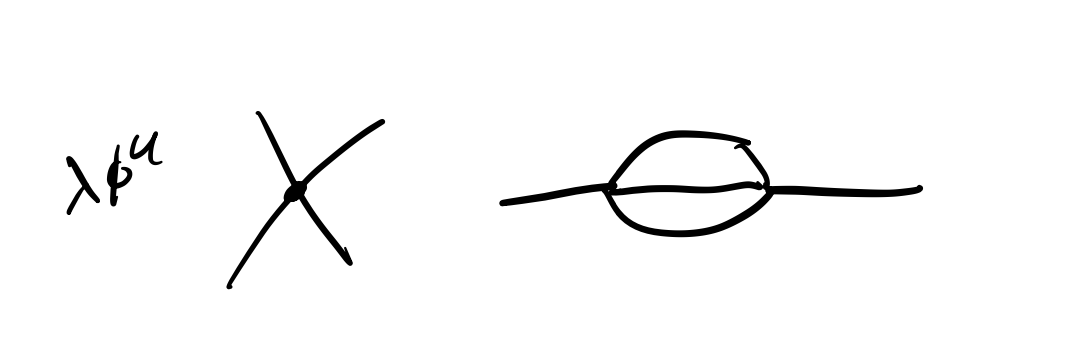
\includegraphics[scale=0.3]{Lectures/Figures/lec13-phi4.png}
\end{center}

where now the particle splits into three particles (the diagram on the right corresponds to the momentum space diagram), so the experimentalist would see a there-particle continuum starting at $3m$.

\subsection{Comments}
\begin{enumerate}
    \item Why have we written $G(p) = \frac{-i}{p^2 + m^2 - \Pi(p)}$ if $\Pi(p) = O(\lambda^2) + \ldots$? We do not know all $O(\lambda^4)$ diagrams. We can draw them:
    \begin{center}
        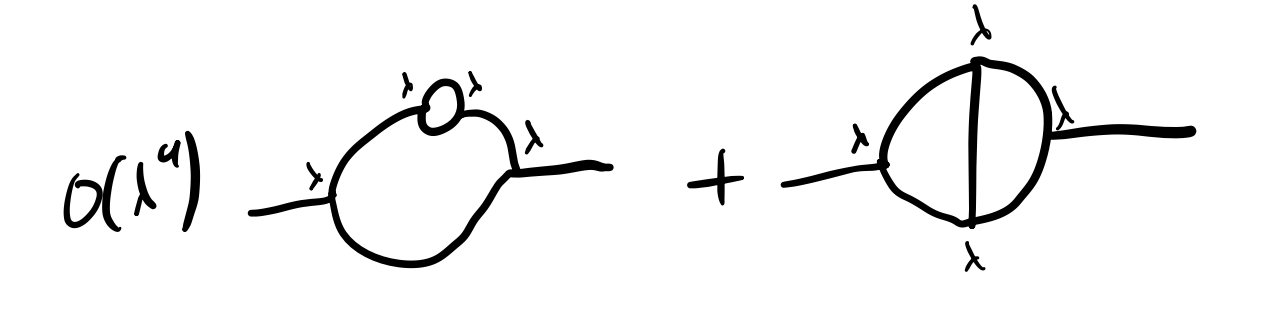
\includegraphics[scale=0.3]{Lectures/Figures/lec13-lambda4.png}
    \end{center}
    but we did not include them. Why? The answer is that often, we are interested in $G_{\text{int}}(p)$ near its pole, where it is largest, i.e. near $p^2 \approx -m^2$. In this regime, the diagrams involving the largest amount of bare propagators, i.e. the largest number of $G(p^2)$s, give the largest contribution. Phrased another way, we are computing small corrections to things (we are working in perturbation theory). If there is a small correction and/or branch cut to the location of the pole, there is a huge correction to the Green's function. Compare the one-loop diagrams (and geometric series of them) with the other $O(\lambda^4)$ diagrams we drew above; they have less factors of $G(p^2)$ and thus contribute less. Having already computed the one-loop diagram and packaging it in $\Pi(p)$ (and hence the correction to $G(p)$ as a geometric series), we have already found the largest contribution.
    \begin{center}
        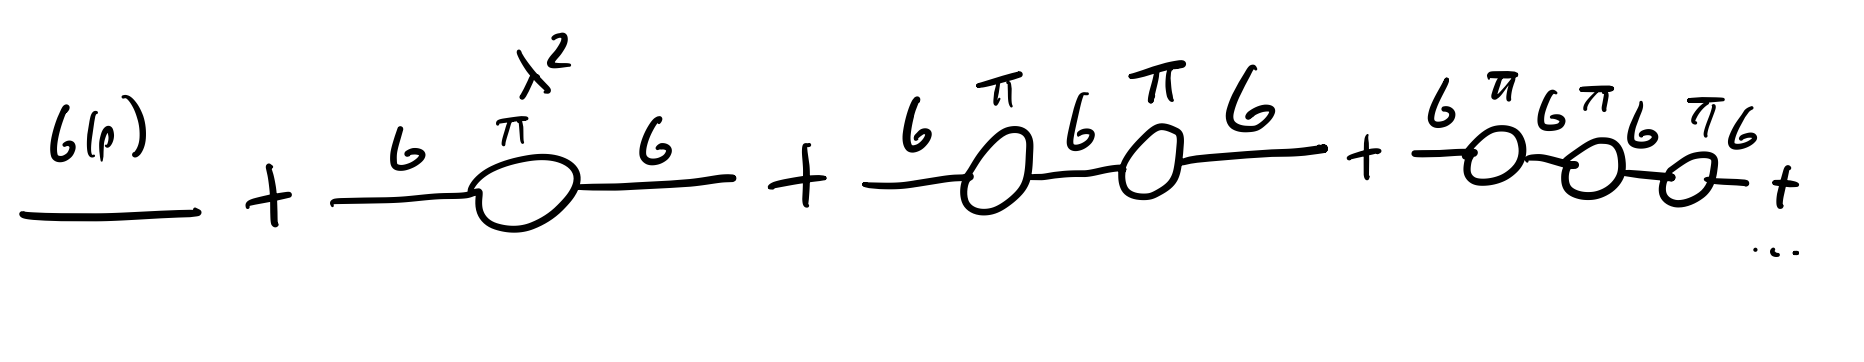
\includegraphics[scale=0.3]{Lectures/Figures/lec13-geomseries.png}
    \end{center}

    Another, related comment; $\Pi(p)$ is a good way to repackage perturbation theory as a whole.  To this end, we are really considering the Taylor series expansion of diagrams that cannot be separated into two with a cut of a single line, also  are know as ``1PI'', or 1-particle irreducible diagrams. Another way to describe them is that there are no intermediate single-particle states. Going to higher order:
    \begin{equation}
        G(p) = \frac{-i}{p^2 + m^2 - \Pi(p)}
    \end{equation}
    already resums the geometric series for any building block. At higher orders this building block contains more complicated objects (more 1PI diagrams exist). But, the general fact is that the Green's function contains all connected diagrams, but they are organized as geometric series in the 1PI diagrams:
    \begin{center}
        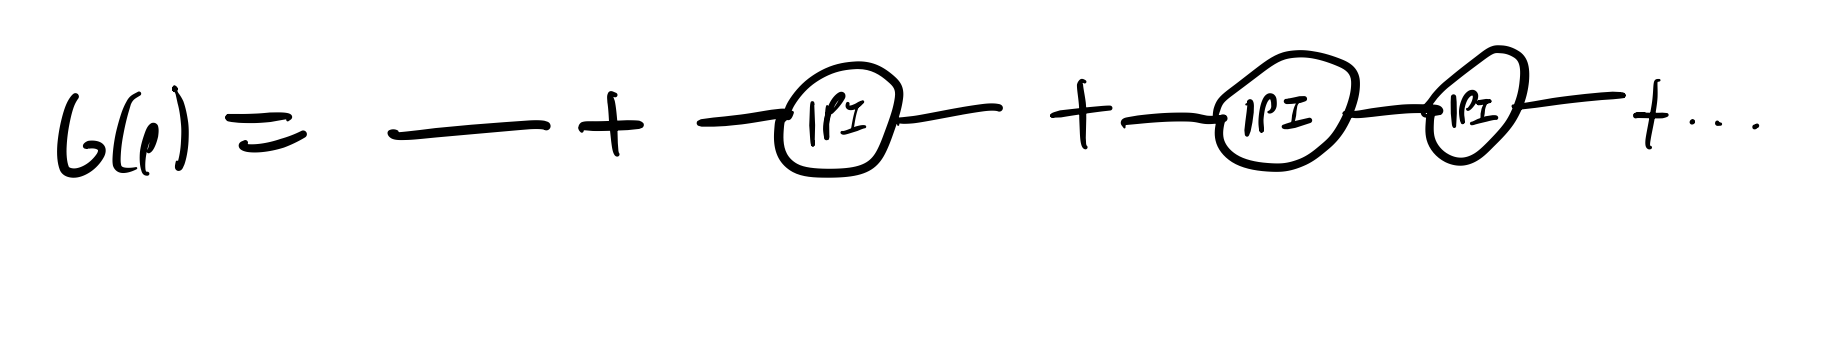
\includegraphics[scale=0.3]{Lectures/Figures/lec13-1PIgeomseries.png}
    \end{center}
    
    Thus, we can equate $\Pi(p)$ with all 1PI diagrams. The 1PI diagrams to $\lambda^4$ in perturbation theory look like:
    \begin{center}
        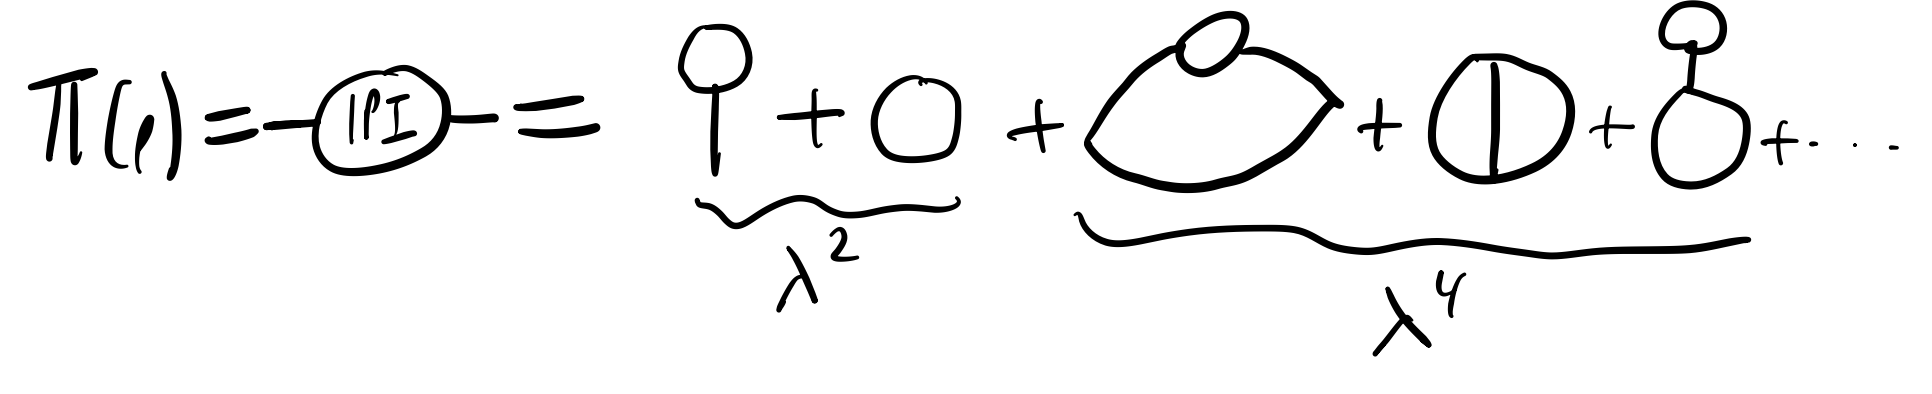
\includegraphics[scale=0.3]{Lectures/Figures/lec13-1PIlambda4.png}
    \end{center}

    \item A second small comment. Physical quantities do \emph{not} depend on the regulator. For the location of the pole/$m_{\text{phys}}^2$, this is a tautological statement, because we did not predict anything. But the location of the branch point at $4m_{\text{phys}}^2$, and the value of the Green's function along the branch cut is something that \emph{cannot} be modified by the choice of the regulator. The UV divergences are helpful in the sense that they tell us where we have predictive power, and where we do not.
    
    \item We are doing perturbation theory in $\lambda$. But of course $\lambda$ is a dimensionful quantity, so saying it is ``small'' does not make much sense on its own. What is the small dimensionless parameter that is giving us control over the expansion? $[\lambda] = \frac{6-D}{2}$, or $\lambda \sim E^{\frac{6-D}{2}}$. In fact, the dimensionless number depends on the energy scale; for example $\frac{\lambda}{p^{\frac{6-D}{2}}}$. For PT to work/be controlled, we need the above dimensionless quantity to be small. More specifically, if $[\lambda] > 0$ (as is the case for $D < 6$), we require the interaction to be large to have control. 
    Interactions are \emph{relevant}, it has a large effect at low energies. Perturbation theory works at high energy in this case. Conversely, if $[\lambda] < 0$ ($D > 6$), then interactions are \emph{irrelevant}, i.e. it has a small effect at low energies. Thus perturbation theory works at $p \ll \lambda^{\#}$. This is the regime of EFT. What if $[\lambda] = 0$, i.e. precisely at $D = 6$? Then, we compare $\lambda$ to $\log(p)$, and we have $G(p) = \frac{1}{p^2}(1 + \lambda^2 \log(p))$. In this case, PT breaks down both at high and low energies. Unfortuantely, it is the case that most couplings in the universe (in the standard model) are dimensionless. What ends up saving us is the renormalization group, which we discuss next day.
\end{enumerate}
\newpage
\section{The Renormalization Group}
\subsection{When is perturbation theory any good? - A classification of couplings}
We revisit the last comment from our previous lecture. We had noticed that couplings are (typically) dimensionful, and hence it is not meaningful to say they are ``small''. E.g. $[\lambda_{\phi^3}] = \frac{D-6}{2}$. So, really the expansion parameter is not the coupling, but the coupling times some energy scale; $\lambda_{\phi^3}/E^{\frac{6-D}{2}} \ll 1$. This depends on what observable we study, and influences where perturbation theory works.

In the example that we computed, if we set $m = 0$ then:
\begin{equation}
    G_{\text{int}}(p) = \frac{-i}{p^2}\left(1 + C\frac{\lambda^2}{(p^2)^{[\lambda]}} + \ldots\right)
\end{equation}
The energy scale is set by $p^2$, i.e. $E \sim \sqrt{p^2}$. Depending on the dimensions our notion of ``small'' changes.

\emph{Relevant couplings} are those with $[\lambda] > 0$. Then, the perturbation theory is controlled at high energies (compared to the coupling). Theories with only relevant interactions/couplings are called \emph{asymptotically free} (at high energies, they become free). They have the property of being \emph{UV-complete}, because in principle they provide a complete microscopic definition of a theory. They are also called \emph{renormalizable} (though this is older, and arguably questionable, terminology).

\emph{Irrelevant couplings} are those with $[\lambda] < 0$. Then, perturbation theory is controlled at low energies (compared to the coupling). QFTs with irrelevant couplings are known as ``effective field theories'' - they cannot be theories of everything (there is a more complete theory at higher energy/shorter length scales, and the UV is unknown) but still can be massively useful in making predictions.

\begin{center}
    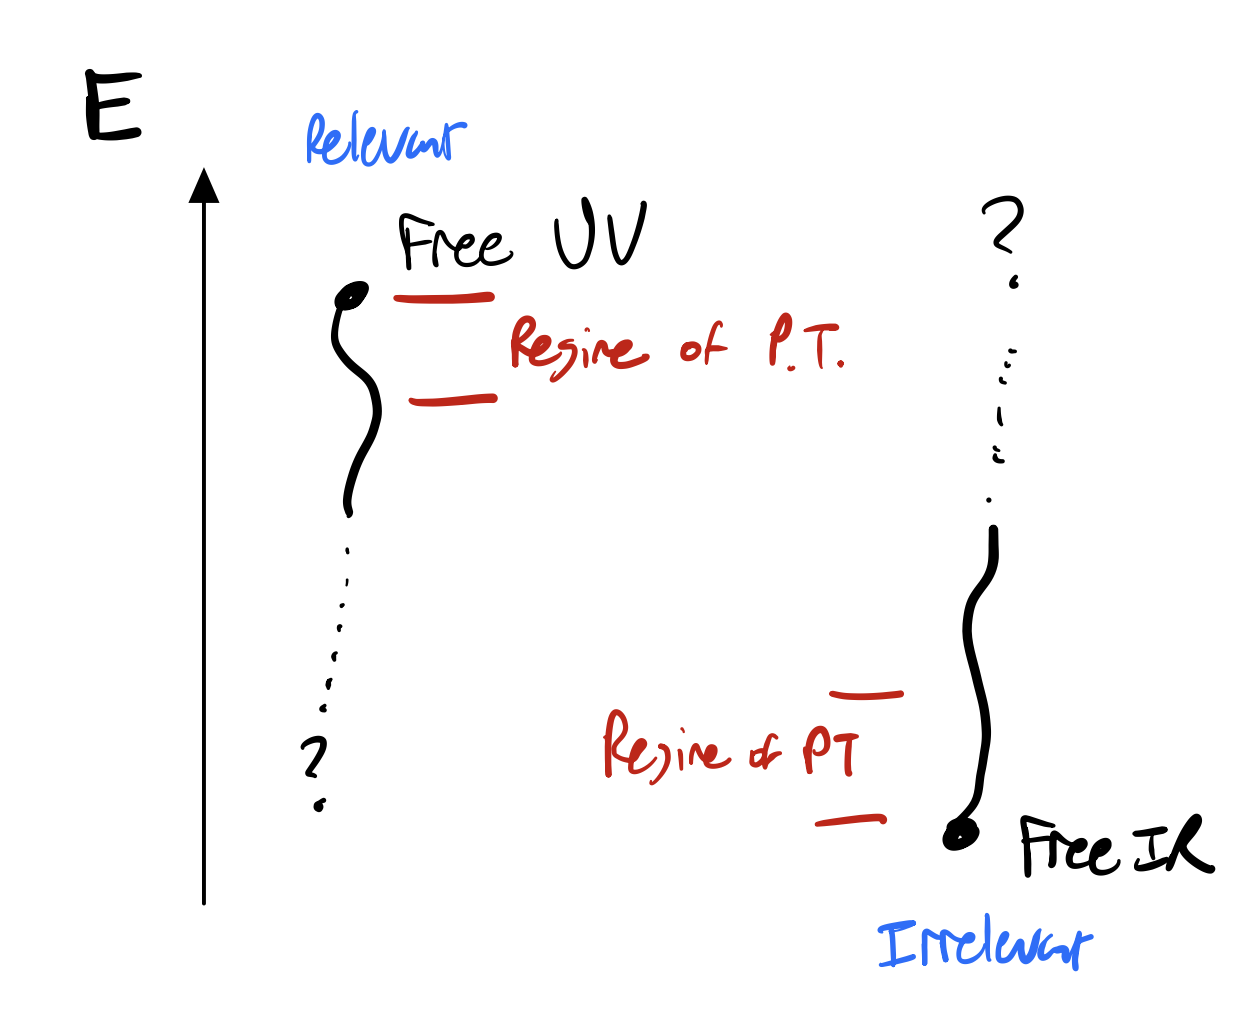
\includegraphics[scale=0.4]{Lectures/Figures/lec14-ptvalidity.png}
\end{center}

\emph{Marginal couplings} are those with $[\lambda] = 0$. This would be the $D = 6$ case for the $\phi^3$ theory. This seems like a fine-tuned example, but actually applies to many interesting theories, e.g. QED. In this case, if we compute the loop corrections, they do not give power law corrections to the momenta, but rather (dimensionless) logarithms. E.g. looking at the non-analytic part of the correction in $\phi^3$ theory:
\begin{equation}
    G_{\text{int}}(p) = \frac{-i}{p^2}\left(1 + \lambda^2 \log \frac{p}{\Lambda} + \ldots\right)
\end{equation}
Now the issue here is that the perturbation theory seems to break down when both $p \to 0$ and $p \to \infty$. Said another way, we see a breakdown both at high/low energies, or both in the UV and the IR. So is PT actually useless here? Actually, slightly more careful analysis will save the day, and will show that marginal couplings also become large in the UV \emph{or} the IR, not both. We can thus consider such couplings as either marginally relevant or irrelevant. However, we have to go beyond simple dimensional analysis to figure this out. It will be theory dependent. The machinery that will allow us to tackle this is the \emph{renormalization group}.

\subsection{Motivating/Introducing the Renormalization Group}
Pragmatically, RG will allow us to ``resum the logarithms'' for theories with marginal couplings, recovering controlled perturbative predictions. But, it has deep consequences beyond this. For one, it connects particle physics with statistical mechanics. Additionally, it introduces the possibility of special quantum field theories, known as conformal field theories (CFTs) which are fixed points of the renormalization group. RG asks ``what happens as we change scales in a theory?'' and CFTs are special theories that are scale invariant. Originally when CFTs were introduced, they were originally thought as special theories with no experimental consequence (as our world is full of scale-dependent thing) but now they are seen in a different light; they are seen as special corners of theories which can make predictions via addition of different couplings. They are very powerful, allowing for non-perturbative approaches to QFT. They also give a way to define string theory.

RG is arguably one of the biggest developments of theoretical physics in the last century\footnote{Was partly developed in Chicago! Invented by Wilson, Kadanoff\ldots}. Conceptually, we want to ask the question of ``how does a theory change under coarse graining''? We may have some microscopic description of a system, and want to coarse grain. Under this coarse graining, the original microscopic action $S$ will map to an effective action $S_{\text{eff}}$ with slightly different effective couplings. 

\begin{center}
    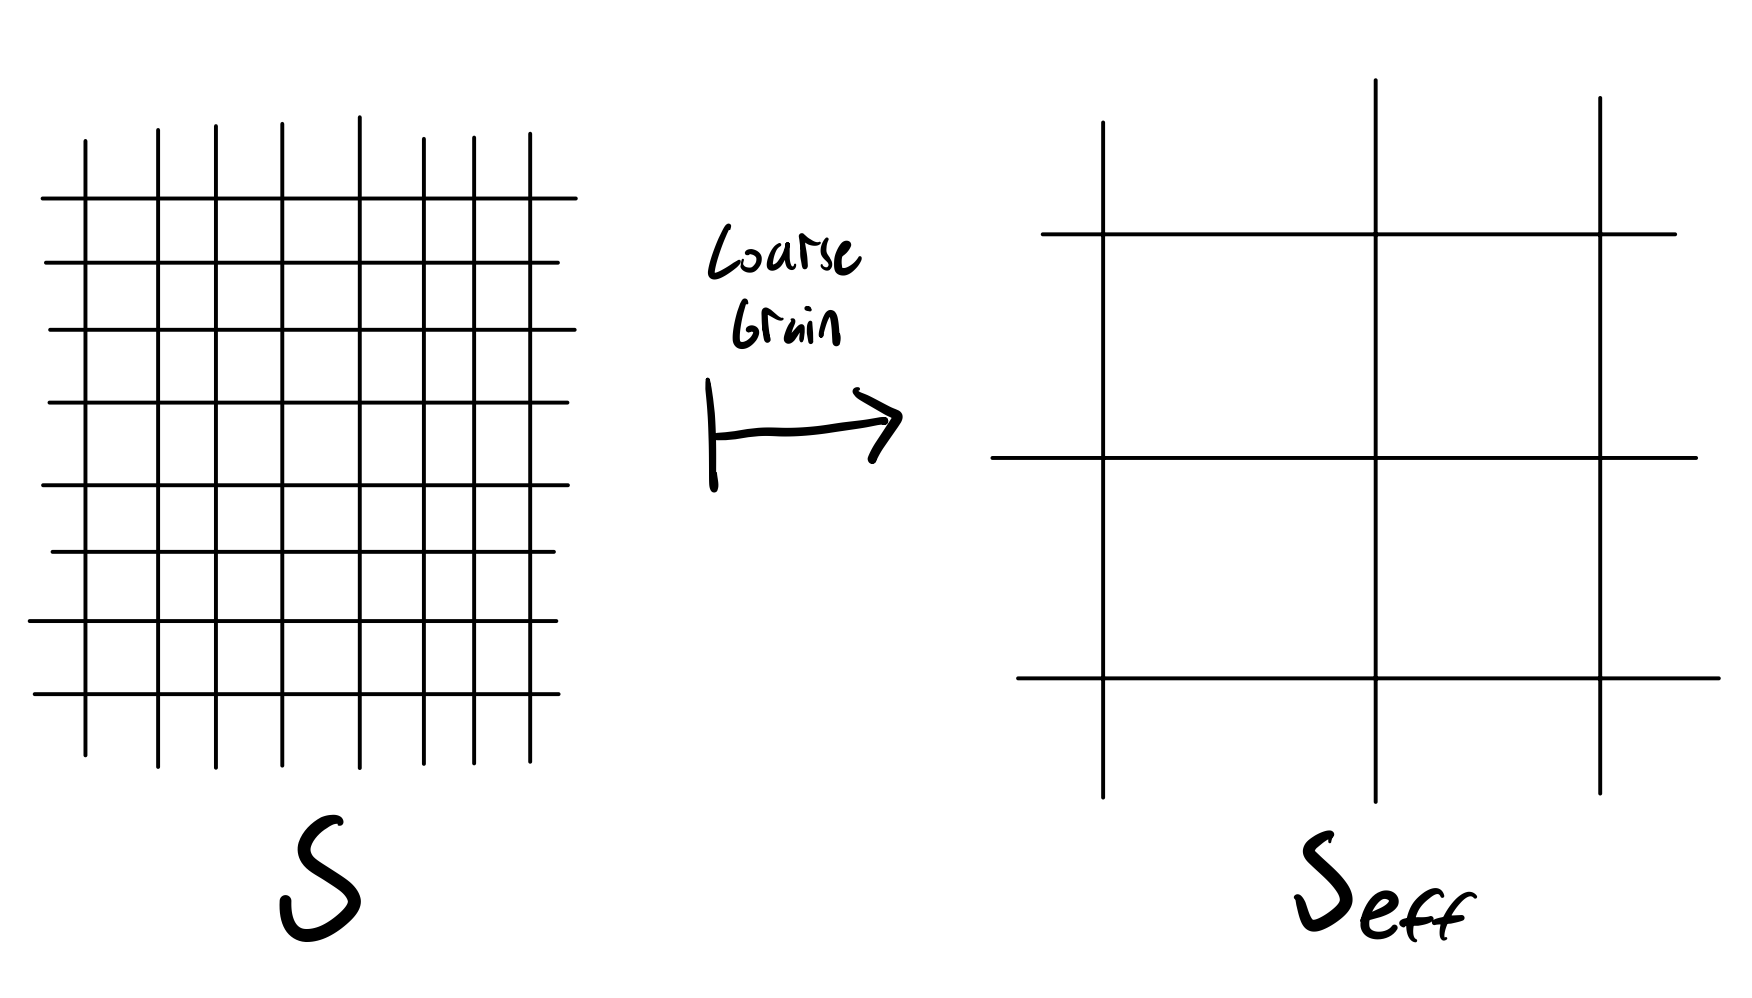
\includegraphics[scale=0.3]{Lectures/Figures/lec14-coarsegrain.png}
\end{center}

Couplings that \emph{grow} are relevant, and those that shrink are irrelevant. This coarse-graining procedure is what is called a renormalization group flow. Pictorially, we imagine that there are flows in the space of theories, where $S$ flows to $S_{\text{eff}}$.

\begin{center}
    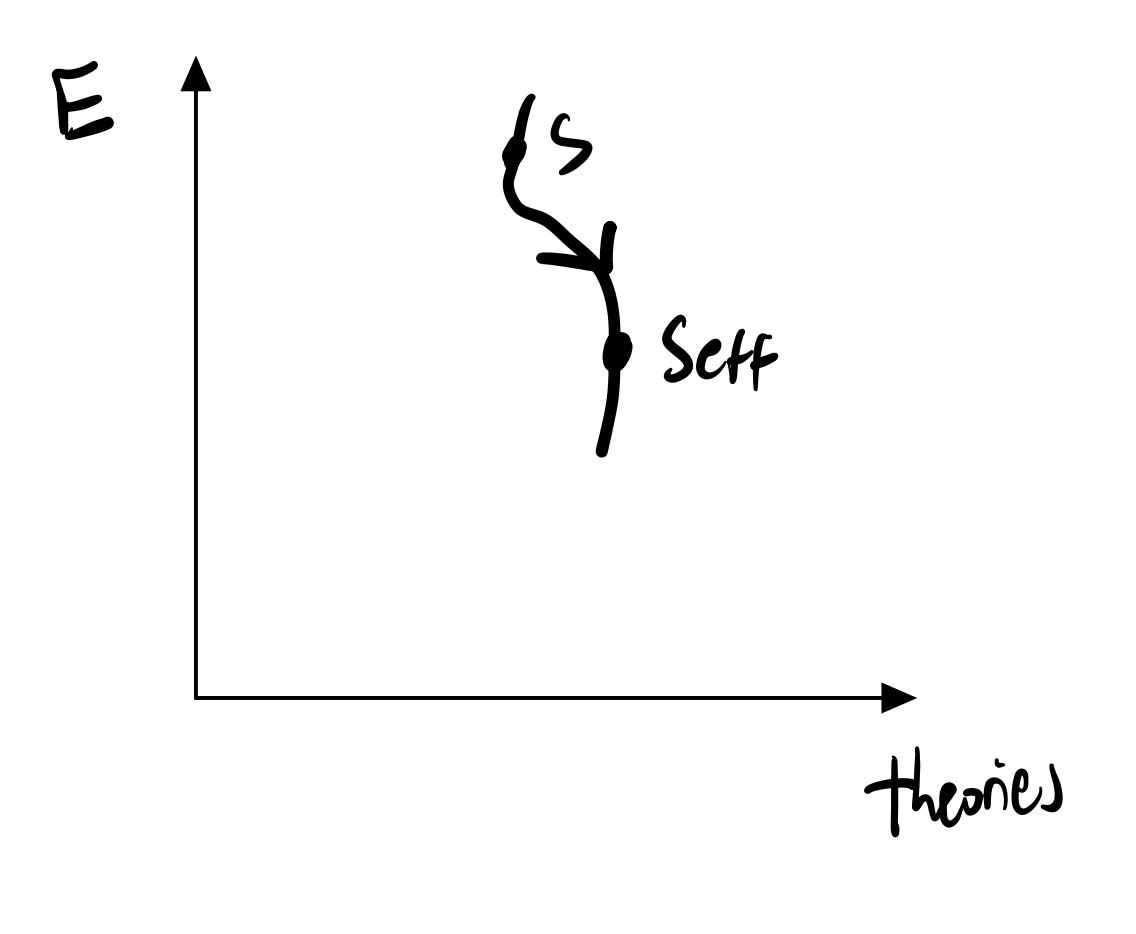
\includegraphics[scale=0.35]{Lectures/Figures/lec14-rgflow.png}
\end{center}

In QFT there is a very elegant way to implement this using the path integral, which we will now begin to explore. A useful reference for this part of the course is Chapter 12 of Peskin and Schroeder.

\subsection{Case Study - Looking at $\phi^4$ theory}
Srednicki uses $\phi^3$, where the interesting questions are in $D = 6$... so let's instead look at $\phi^4$ theory, where there are interesting things happening in $D = 4$ (else Luca would feel bad if this was your only QFT course and you only got to study 6 spacetime dimensions, which is beyond our everyday experience). Our action takes the form:
\begin{equation}
    S = \int d^Dx \frac{1}{2}(\p_\mu \phi)^2 + \frac{1}{2}m^2\phi^2 + \frac{1}{4!}\lambda \phi^4
\end{equation}
Doing dimensional analysis, we have (for the action to be dimensionless):
\begin{equation}
    [\phi] = \frac{D-2}{2}, [m] = 1
\end{equation}
and then looking at the dimension of $\lambda$:
\begin{equation}
    1 \sim \frac{S_{\text{int}}}{S_{\text{m}}} \sim \frac{\lambda\phi^4}{m^2} \sim \lambda E^{D-4} \implies [\lambda] = 4-D
\end{equation}
For $D < 4$, the coupling is relevant (going to higher energies we get more perturbative control). For $D > 4$ it is irrelevant (going to lower energies we get more perturbative control). For $D = 6$ the coupling is marginal, and we don't know (yet) where we need to go to get control over our theory - we need to do more work.

The way we implement RG in QFT using the path integral is quite nice. What we can do is integrate out (path integrate) all fields with momentum beyond/above some value (i.e. energies above a certain scale/below some length scale), and we will see how the couplings flow when we do this. To simplify, let us Wick rotate from the start, $t \to it_E$:
\begin{equation}
    e^{iS} \to e^{-S_E}
\end{equation}
with:
\begin{equation}
    S_E = \int d^Dx \frac{1}{2}(\nabla \phi)^2 + \frac{1}{2}m^2 \phi^2 + \frac{1}{4!}\lambda\phi^4
\end{equation}
now, its quite clear that we are doing statistical mechanics, with $S_E$ taking the role of $\beta H$. Instead of looking at $3+1$ dimensions (3 spatial, 1 time), the problem is now in 4 spatial dimensions. Consider the path integral:

\begin{equation}
    Z = \int \prod_x d\phi(x)e^{-S_E} = \int \prod_k d\phi_k e^{-S_E(\phi_k)}
\end{equation}
We now consider a slightly different object; a path integral where all modes with $k > \Lambda$ have already been integrated out:
\begin{equation}
    Z_\Lambda = \int \prod_{k < \Lambda}d\phi_k e^{-S_E}
\end{equation}
In the coarse graining step, we then integrate out all $\phi_k$ with $b\Lambda < \abs{k} < \Lambda$, with $0 < b < 1$ and $1 - b \ll 1$.

\begin{center}
    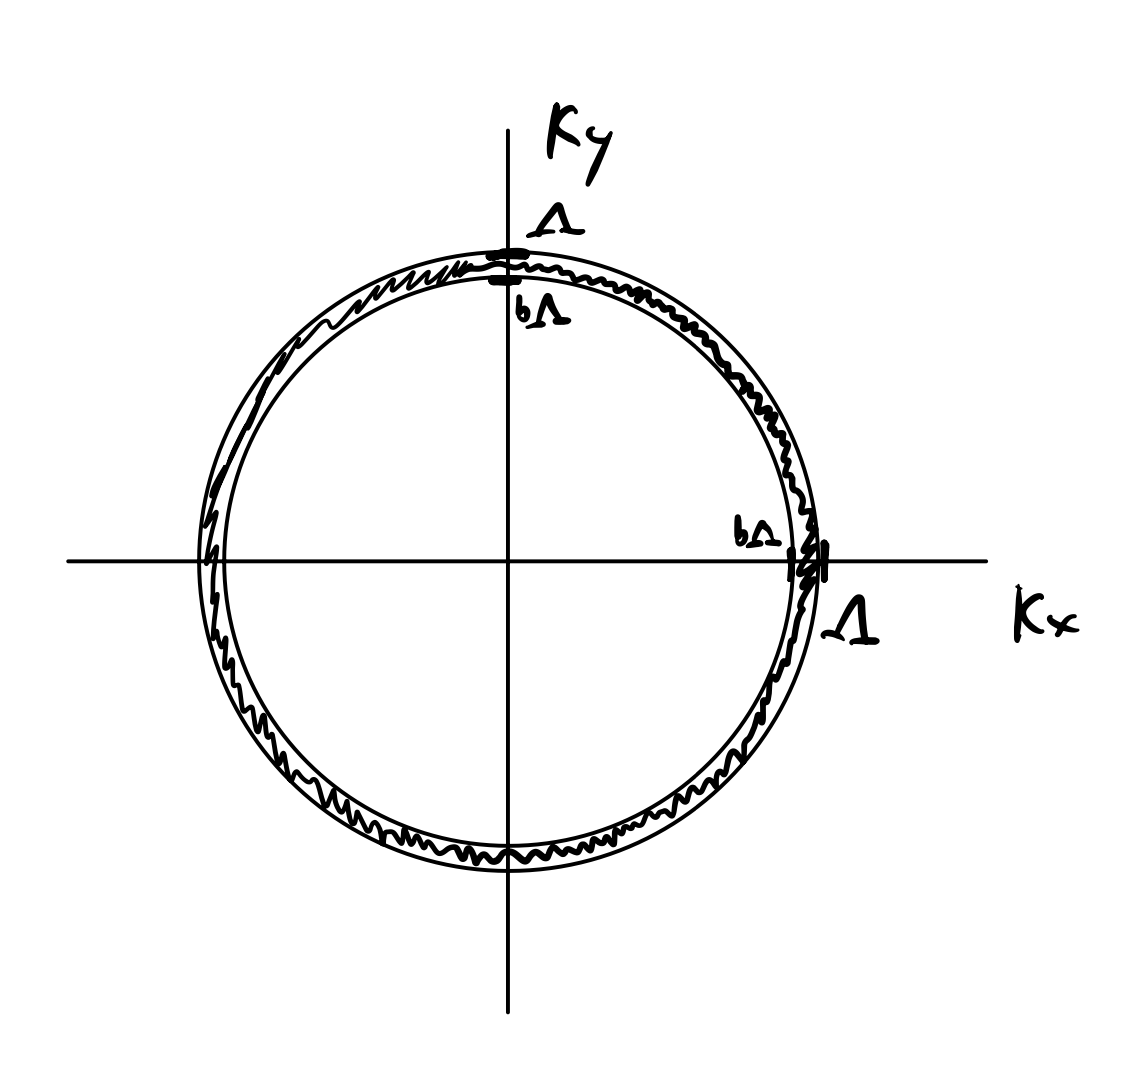
\includegraphics[scale=0.35]{Lectures/Figures/lec14-momentumshell.png}
\end{center}
We then compare to $Z_{\Lambda}$.

\subsection{Free-theory warm-up}
We consider:
\begin{equation}
    S_E = \int d^4x \frac{1}{2}(\nabla \phi)^2 + \frac{1}{2}m^2\phi^2 = \int_{k < \Lambda} \frac{d^4k}{(2\pi)^4}\frac{1}{2}(k^2 + m^2)\phi_{k}\phi_{-k}
\end{equation}
where note that in the free theories the momentum modes do not couple. We've already integrated out modes higher than $\Lambda$. Now, we split this integral:
\begin{equation}
    S_E = \int_{k < b\Lambda}\frac{1}{2}(k^2 + m^2)\phi_k\phi_{-k} + \int_{b\Lambda < k < \Lambda}\frac{1}{2}(k^2 + m^2)\phi'_{k}\phi'_{-k}
\end{equation}
where we use $\phi_k$ to denote modes with $k < b\Lambda$ and $\phi_k'$ to denote modes with $b\Lambda < k < \Lambda$. We then have:
\begin{equation}
    \begin{split}
        Z_\Lambda &= \int \prod_{k < b\Lambda}d\phi_k \int \prod_{b \Lambda < k < \Lambda} d\phi_k' e^{-S}
        \\ &= \int \prod_{k < b\Lambda}d\phi_k e^{-\frac{1}{2}\int_{k < b\Lambda}(k^2 + m^2 \phi_k \phi_{-k})} \int \prod_{b\Lambda < k < \Lambda}d\phi_k' e^{-\frac{1}{2}\int_{b\Lambda < k < \Lambda}(k^2 + m^2)\phi_k'\phi_{-k}'}
    \end{split}
\end{equation}
The integral over the $\phi_k'$s just gives a number independent of $\phi$ (call it $C$) and we are left with just the path integral over the low energy modes:
\begin{equation}
    Z_\Lambda = C\int \prod_{k < b\Lambda}d\phi_k d\phi_k e^{-\frac{1}{2}\int_{k < b\Lambda}\frac{1}{2}(k^2 + m^2)\phi_k \phi_{-k}}
\end{equation}
Now, we want to compare this to what we started with. In order for the range of momenta to match, we substitute $\tilde{k} = \frac{k}{b} < \Lambda$.
\begin{equation}
    Z_\Lambda = \int \prod_{\tilde{k} < \Lambda}d\phi_{\tilde{k}} e^{-\int_{\tilde{k} < \Lambda}\frac{1}{2}b^4(b^2 \tilde{k}^2 + m^2)\phi_{\tilde{k}}\phi_{-\tilde{k}}}
\end{equation}
Now rescale the field $\tilde{\phi} = b^3\phi$ to have a canonical kinetic term:
\begin{equation}
    Z_{\Lambda} = \int \prod_{\tilde{k} < \Lambda}d\phi_{\tilde{k}} e^{-\int_{\tilde{k} < \Lambda}\frac{1}{2}(\tilde{k}^2 + \frac{m^2}{b^2})\phi_{\tilde{k}}\phi_{-\tilde{k}}}
\end{equation}
We see that the effective $m^2$ has grown, with $m^2 \to \frac{m^2}{b^2}$. This is a very complicated way to make a very obvious statement. Recall the propagator of the free scalar is:
\begin{equation}
    G(k) = \frac{1}{k^2 + m^2}
\end{equation}
So all this is saying is that as we decrease the energy $k$, the effect of the mass $m$ grows. Thus, we would say that $m^2$ is \emph{relevant}, because it matters more at low energies/under coarse graining. This is the same thing that we would have obtained by doing dimensional analysis.

Now we have all the ingredients we need to study the renormalization of a $\phi^4$ interacting theory.

\subsection{Back to renormalization of $\phi^4$}
We return to:
\begin{equation}
    S = \int d^4x \frac{1}{2}(\nabla \phi)^2 + \frac{1}{2}m^2 \phi^2 + \frac{1}{4!}\lambda\phi^4
\end{equation}
When we fourier transform the $\phi^4$ term, we get something of the form:
\begin{equation}
    \int_{k_1k_2k_3}\phi_{k_1}\phi_{k_2}\phi_{k_3}\phi_{-k_1-k_2-k_3}
\end{equation}
which is more subtle than what we had before, the RG mixes the high and low energy modes. Suppose we split into $\phi, \phi'$:
\begin{equation}
    S[\phi + \phi'] = \int d^4x \frac{1}{2}(\p(\phi + \phi'))^2 + \frac{1}{2}m^2(\phi + \phi')^2 + \frac{\lambda}{4!}(\phi + \phi')^4
\end{equation}
So looking at the partition function:
\begin{equation}
    Z = \int D\phi e^{-S(\phi)}\int D\phi' \exp(-\int \frac{1}{2}(\p\phi')^2 + \frac{1}{2}m^2\phi'^2 + \frac{\lambda}{4!}(\phi'^4 + 4\phi'^3\phi + 6\phi'^2\phi^2 + 4\phi'\phi^3))
\end{equation}
we see that the last term indeed mixes the high and low energy modes. Let's expand:
\begin{equation}
    Z = \int D\Phi e^{-S(\phi)}\int D\phi' e^{-S(\phi')} [1 - \frac{\lambda}{4!}\int d^4x (4\phi'^3\phi + 6\phi'^2\phi^2 + 4\phi'\phi^3) + \ldots]
\end{equation}
We can view the $\phi$ in the $\phi'$ integral as an external source:
\begin{equation}
    Z = \int D\Phi e^{-S(\phi)}\left(1 - \frac{\lambda}{4!}\int d^4x 4\phi(x)\avg{\phi'^3(x)} + 6\phi^2(x)\avg{\phi'^2(x)} + 4\phi^3(x)\avg{\phi'(x)}\right)
\end{equation}
now, by the $\mathbb{Z}_2$ symmetry of the theory the one and three point functions vanish, so we are left with:
\begin{equation}
    Z = \int D\Phi e^{-S(\phi)}\left(1 - \frac{\lambda}{4!}\int d^4x + 6\phi^2(x)\avg{\phi'^2(x)}\right)
\end{equation}
Diagramatically, the contribution of this term looks like:

\begin{center}
    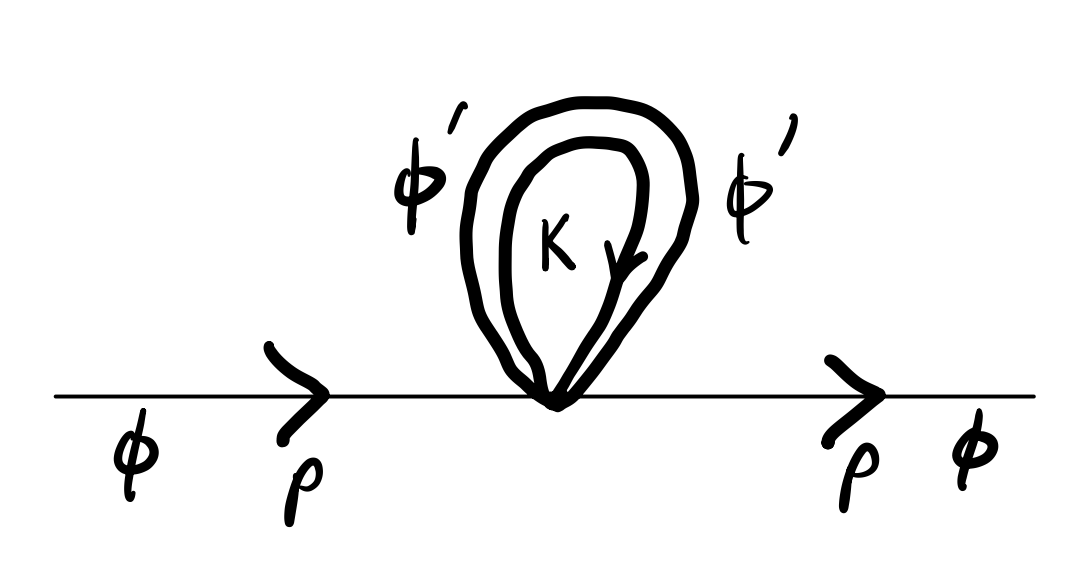
\includegraphics[scale=0.35]{Lectures/Figures/lec14-massrenorm.png}
\end{center}

Let's compute the two point function. This is similar to the free field two-point function we know, but we only integrate over the modes between $b\Lambda$ and $\Lambda$:
\begin{equation}
    \avg{\hat{\phi}'^2(x)} = \avg{\phi'(x)\phi'(x)} = \int_{b\Lambda < k < \Lambda}\frac{d^4k}{(2\pi)^4}\frac{1}{k^2 + m^2} = \frac{2\pi^2}{(2\pi)^4}\int_{b\Lambda}^\Lambda dk \frac{k^3}{k^2 + m^2}
\end{equation}
Now if we assume that $m \gg \Lambda$, then since $k \sim \Lambda$ we have:
\begin{equation}
    \avg{\hat{\phi}'^2(x)} \approx \frac{1}{8\pi^2}\int_{b\Lambda}^\Lambda dkk = \frac{1}{16\pi^2}(\Lambda^2 - (b\Lambda)^2) = \frac{\Lambda^2}{(4\pi)^2}(1 - b^2).
\end{equation}
Thus, we see that the effect of the interaction at this order is to add a term in the path integral for the low energy modes:
\begin{equation}
    Z = \int D\phi e^{-S(\phi)}\left(1 - \frac{\lambda}{2}\int d^4x \phi^2(x)\frac{\Lambda^2}{(4\pi)^2}(1 - b^2) + \ldots \right)
\end{equation}
We reinterpret this small quantity as an exponential:
\begin{equation}
    \exp(-\delta S), \quad \delta S = \frac{1}{2}\int d^4x \frac{\lambda \Lambda^2}{(4\pi)^2}(1 - b)^2\phi^2(x)
\end{equation}
so what did this interaction do? It renormalized the mass by the above amount, so the effective action is now:
\begin{equation}
    S_{\text{eff}} = \frac{1}{2}\int (\nabla \phi)^2 + (m^2 + \delta m^2)\phi^2
\end{equation}
where the mass gets ``dressed'' by the high energy modes. Next week, we will look at higher orders, and we will see that the interactions also renormalize themselves!! (We will then see the fate of $\lambda$!) For example at $O(\lambda^2) $, we will have the contribution:

\begin{center}
    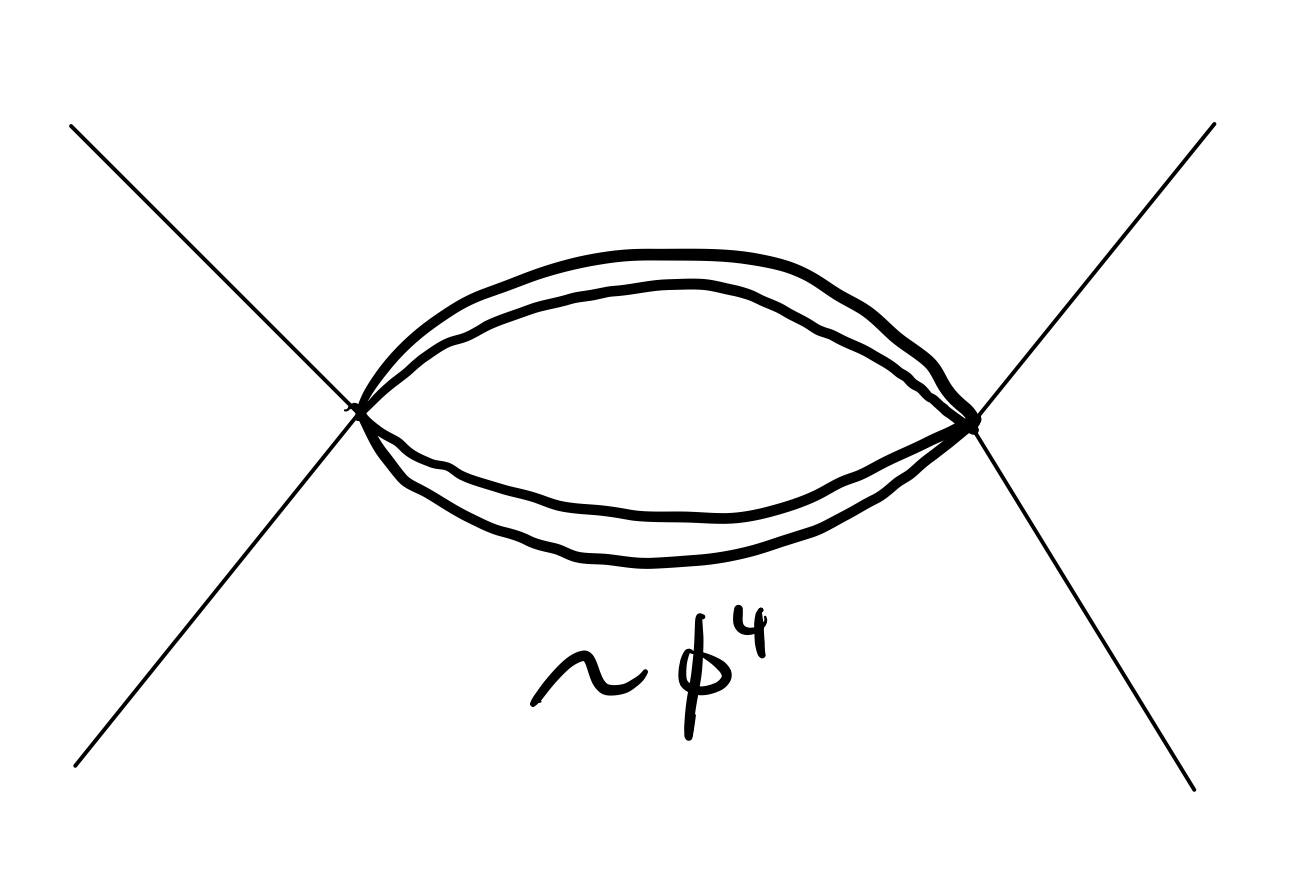
\includegraphics[scale=0.35]{Lectures/Figures/lec14-interactionrenorm.png}
\end{center}




\newpage
\section{Renormalization Group Flows}
\subsection{Review}
We studied how couplings ``flow'' upon integrating out a thin shell $b\Lambda < p < \Lambda$

\begin{center}
    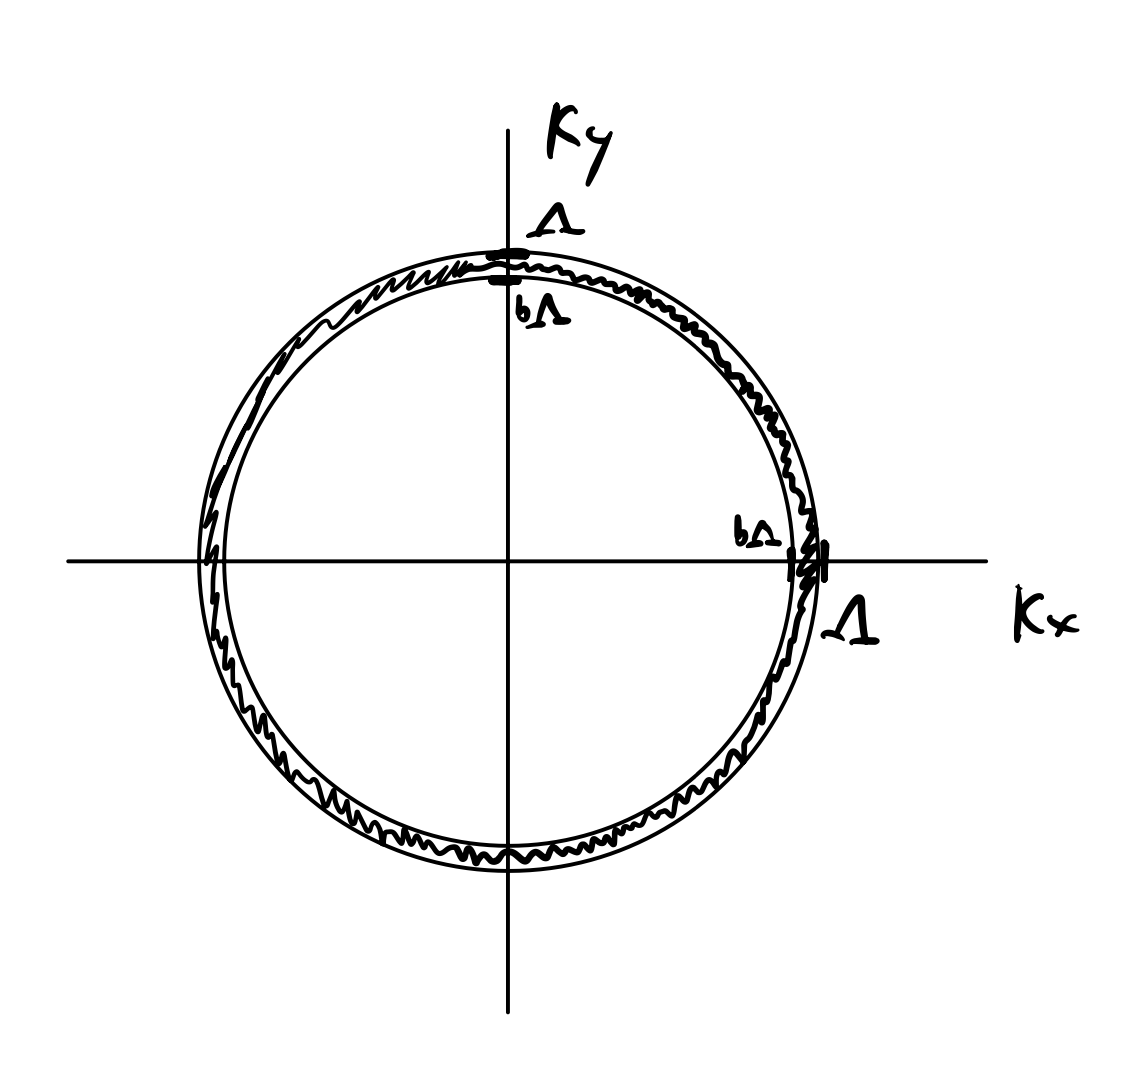
\includegraphics[scale=0.35]{Lectures/Figures/lec14-momentumshell.png}
\end{center}

(should be $p$ in the figure above, but I got lazy and did not want to redraw it). We considered the action:
\begin{equation}
    S = \int d^4x \frac{1}{2}(\nabla \phi)^2 + \frac{1}{2}m^2\phi^2 + \frac{\lambda}{4!}\phi^4
\end{equation}
upon integrating out the field, we had:
\begin{equation}
    Z = \int \mathcal{D}\phi e^{-S[\phi]}\int D\phi' e^{-S_{\text{int}}[\phi, \phi']}e^{-S[\phi']} = \int \mathcal{D}\phi e^{-S_{\text{eff}}[\phi]}
\end{equation}
Expanding in the interaction:
\begin{equation}
    Z = \int \mathcal{D}\phi \int \mathcal{D}\phi' (1 - S_{\text{int}} + \frac{1}{2}S_{\text{int}}^2 + ldots)e^{-S[\phi']}
\end{equation}
Where:
\begin{equation}
    S_{\text{int}} = \frac{\lambda}{4!}\int d^4x 4\phi^3\phi' + 6\phi^2\phi'^2 + 4\phi\phi'^3.
\end{equation}
Then to $O(\lambda)$:
\begin{equation}
    Z = \int \mathcal{D}\phi e^{-S[\phi]}\left(1 - \frac{\lambda}{4}\int d^4x \phi^2 \avg{\phi'^2(x)} + \ldots\right)
\end{equation}
where:
\begin{equation}
    \avg{\phi'^2(x)} = \frac{\Lambda^2}{(4\pi)^2}(1 - b^2)
\end{equation}
Thus:
\begin{equation}
    Z = \int \mathcal{D}\phi e^{-S[\phi]}\left(1 - \int \frac{1}{2}\Delta m^2 \phi^2\right)
\end{equation}
With:
\begin{equation}
    \Delta m^2 = \frac{\lambda\Lambda^2}{2(4\pi)^2}(1 - b^2).
\end{equation}
This contribution is pictorially depicted in the diagrams:

\begin{center}
    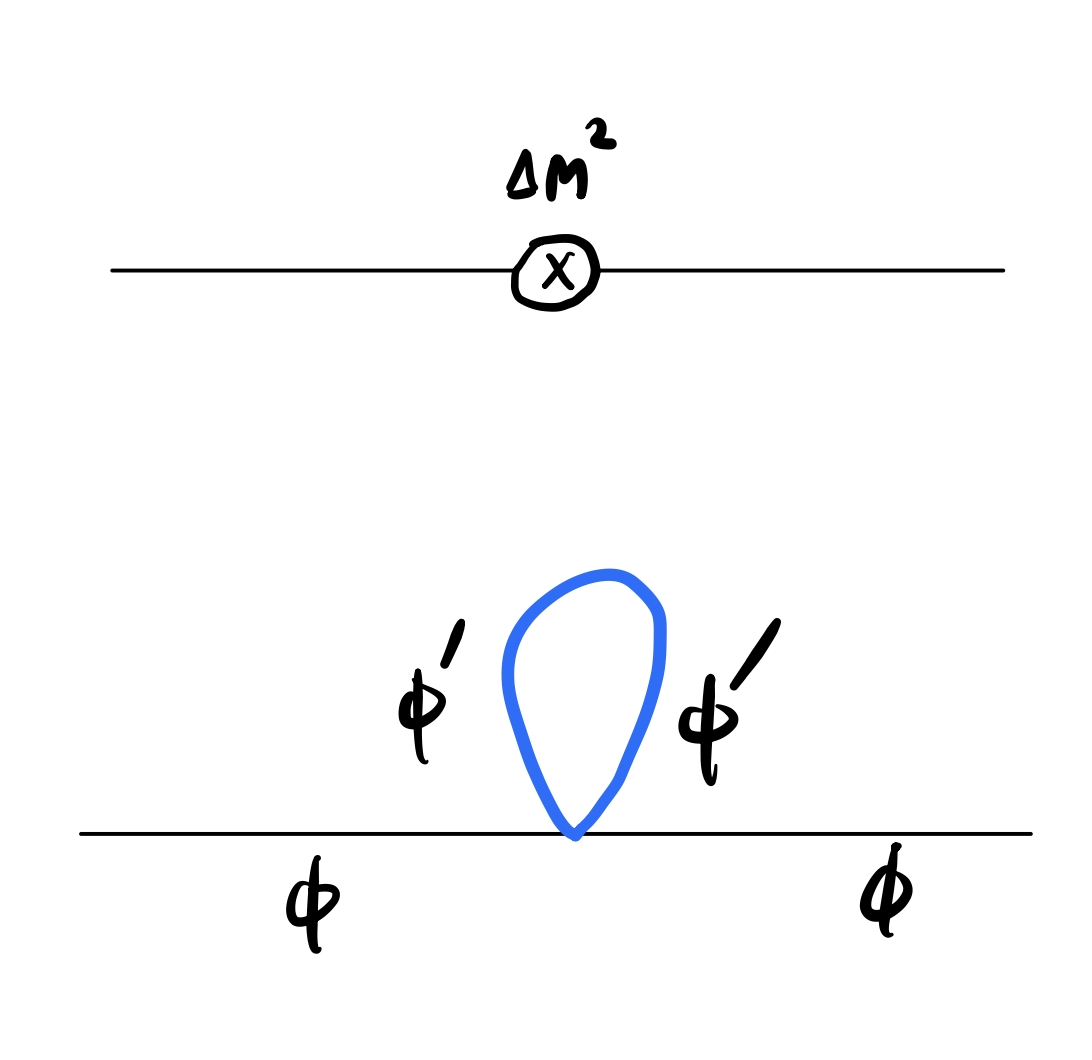
\includegraphics[scale=0.3]{Lectures/Figures/lec15-masscorrection.png}
\end{center}

This isn't so interesting, because the shift of the mass term is just a shift in the classical action. But the renormalization of the \emph{couplings} will be very interesting. This will be particularly interesting when we have theories with dimensionless couplings, when we can't use dimensional analysis to conclude that the coupling is relevant or irrelevant. The flow of the couplings will teach us this information.

\subsection{Renormalizing the interaction}
At higher orders, interactions renormalizes interactions; we have contributions from diagrams like:

\begin{center}
    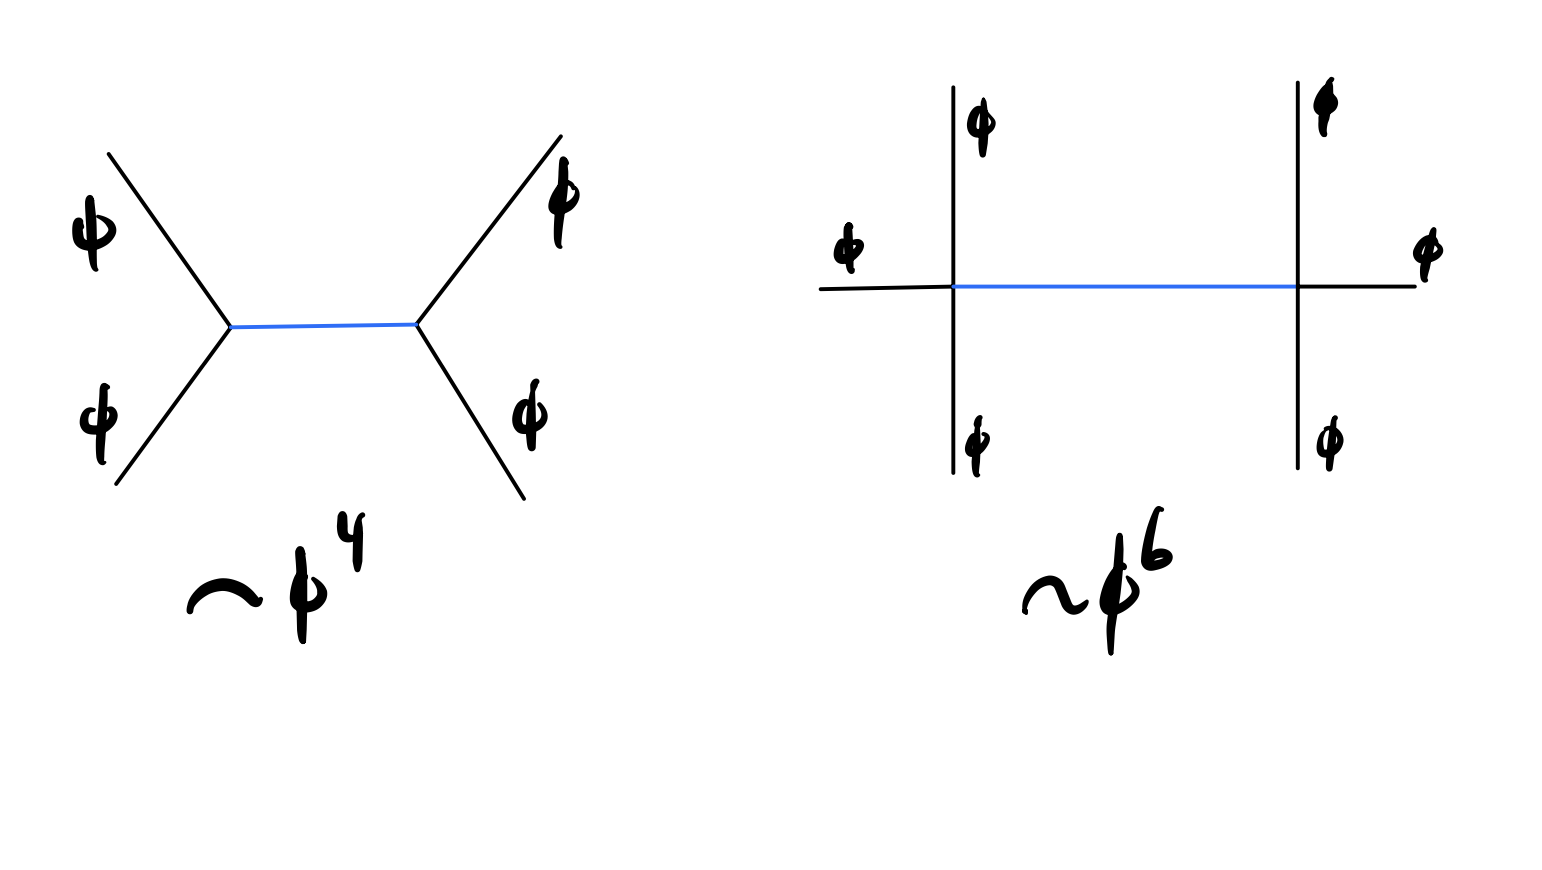
\includegraphics[scale=0.3]{Lectures/Figures/lec15-diagrams.png}
\end{center}

It is worth noting that at this order of $O(\lambda^2)$, several terms/diagrams contribute, but we focus on terms with 4 external fields, as these are the ones that will enter the renormalization of our interaction.

We look at:
\begin{equation}
    S_{\text{int}} = \frac{\lambda}{4}\int d^4x \phi^2(x)\phi'^2(x)
\end{equation}
What we are supposed to compute here is:
\begin{equation}
    Z = \int \mathcal{D}\phi e^{-S}\int \mathcal{D}\phi'\left(1 + S_{\text{int}} + \frac{1}{2}S_{\text{int}}^2 + \ldots \right)e^{-S[\phi']}
\end{equation}
we then need to compute:
\begin{equation}
    (A) = \frac{1}{2}\left(\frac{\lambda}{4}\right)^2\int d^4x d^4x' \phi^2(x)\phi^2(x')\avg{\phi'^2(x)\phi'^2(x')}.
\end{equation}

Where due to Wick contractions the four-point function appearing above just gives us a term $2G(x - x')^2$. This is a loop diagram, and its not too hard to compute. As usual, we work in momentum space:

\begin{center}
    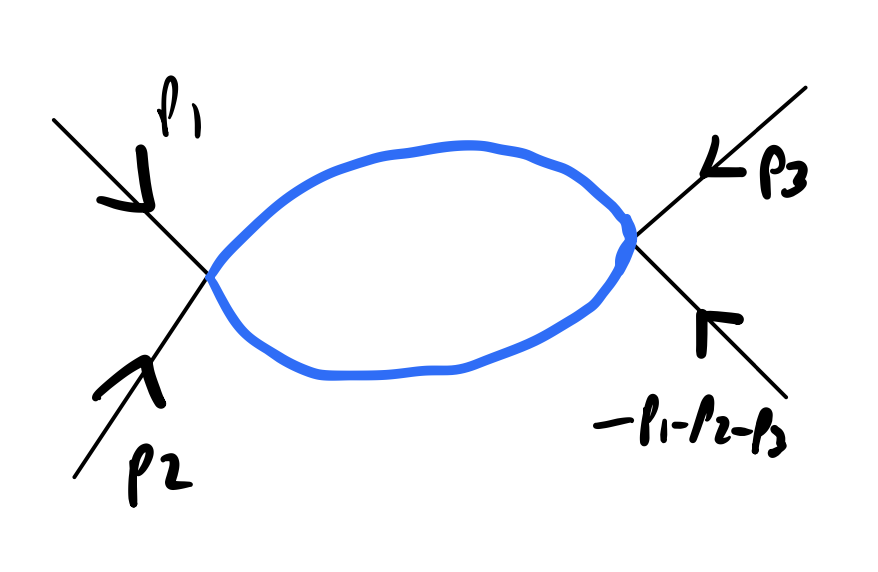
\includegraphics[scale=0.3]{Lectures/Figures/lec15-momentum.png}
\end{center}

so the term is:
\begin{equation}
    (A) = \left(\frac{\lambda}{4}\right)^2\int_{p_1p_2p_3}\phi_{p_1}\phi_{p_2}\phi_{p_3}\phi_{-p_1-p_2-p_3}\int_{p'}G(p')G(-p')
\end{equation}
Assuming $\Lambda \gg p_1, p_2, p_3$ and $\Lambda \gg m$, The $p'$ integral (only in the small shell near $\Lambda$) appearing above gives:
\begin{equation}
    \int_{p'}G(p')G(-p') = \int \frac{d^4p'}{(2\pi)^4}\frac{1}{(p')^4} = \frac{2\pi^2}{(2\pi)^4}\int_{b\Lambda}^\Lambda \frac{dp'}{p'} = \frac{1}{8\pi^2}\log \frac{1}{b}
\end{equation}
So Fourier transforming back, we obtain a correction which we interpret as a correction to the coupling:
\begin{equation}
    Z = \int \mathcal{D}\phi e^{-S[\phi]}\left(1 - \frac{\Delta \lambda}{4!}\int_x \phi^4(x) + \ldots\right)
\end{equation}
with:
\begin{equation}
    \Delta \lambda = -\frac{3\lambda^2}{(4\pi)^2}\log \frac{1}{b} < 0.
\end{equation}
Thus, we found that the effective coupling decreased. What this tells us is that as we go to lower and lower energies (as we coarse grain), the coupling becomes weaker and weaker. Thus, perturbation theory should become more controlled, and at very low energies the theory should become free. At tree level, studying the dimensions we concluded it was marginal. With our more careful analysis here, we found that the coupling is \emph{marginally irrelevant}. Examples of QFTs with marginally irrelevant couplings are:
\begin{itemize}
    \item $\phi^4$ theory in $D = 4$ or $D = 3 + 1$
    \item QED in $D = 4$
    \item Hydrodynamics in $D = 2 + 1$
\end{itemize}
A certain time ago, researchers thought that perhaps all theories were this way. However, this is not the case; examples of QFT with marginally relevant couplings are:
\begin{itemize}
    \item QCD in $D = 4$
    \item BCS theory of superconductivity in any dimension
    \item Non-linear $\sigma$ models in $D = 2$
\end{itemize}

Philosophical aside - RG tells us that we can't live in more than 4 dimensions, because in more than 4 dimensions we can't have dimensionless couplings (up to ongoing research). But for gravity we want $D \geq 4$. So $D = 4$ is the sweet spot.

\subsection{The $\beta$ function}
The $\beta$ function characterizes how the coupling changes with scale. Luca never remembers the sign convention, but it is defined as:
\begin{equation}
    \beta_\lambda = \dod{\lambda}{\log b}
\end{equation}
so for $\lambda \phi^4 > 0$ we have:
\begin{equation}
    \beta_\lambda = \frac{3\lambda^2}{(4\pi)^2} > 0.
\end{equation}
Thus we have that the coupling is marginally irrelevant if $\beta > 0$ and relevant if $\beta < 0$. In PS8, we will look at a case where the $\beta$ function vanishes due to competition of two terms. This is a situation where the theory is scale invariant, and corresponds to a RG fixed point.

\subsection{Callan-Symmezik Equation}
So - we learned how couplings can flow under coarse graining, but we still have the problem of the logarithmic corrections for marginal couplings. How can we use what we have learned to regain control of our perturbation expansion and make predictions for our observables? This brings us to the Callan-Symmezik equation. It is discussed in full generality in Peskin 12.3; here we study a simpler version.

The simplest thing we could use to probe the coupling is the four point function (we will see later that this can also be interpreted as a 2-to-2 scattering) $\avg{\phi_{p_1}\phi_{p_2}\phi_{p_3}\phi_{-p_1-p_2-p_3}}$:

\begin{center}
    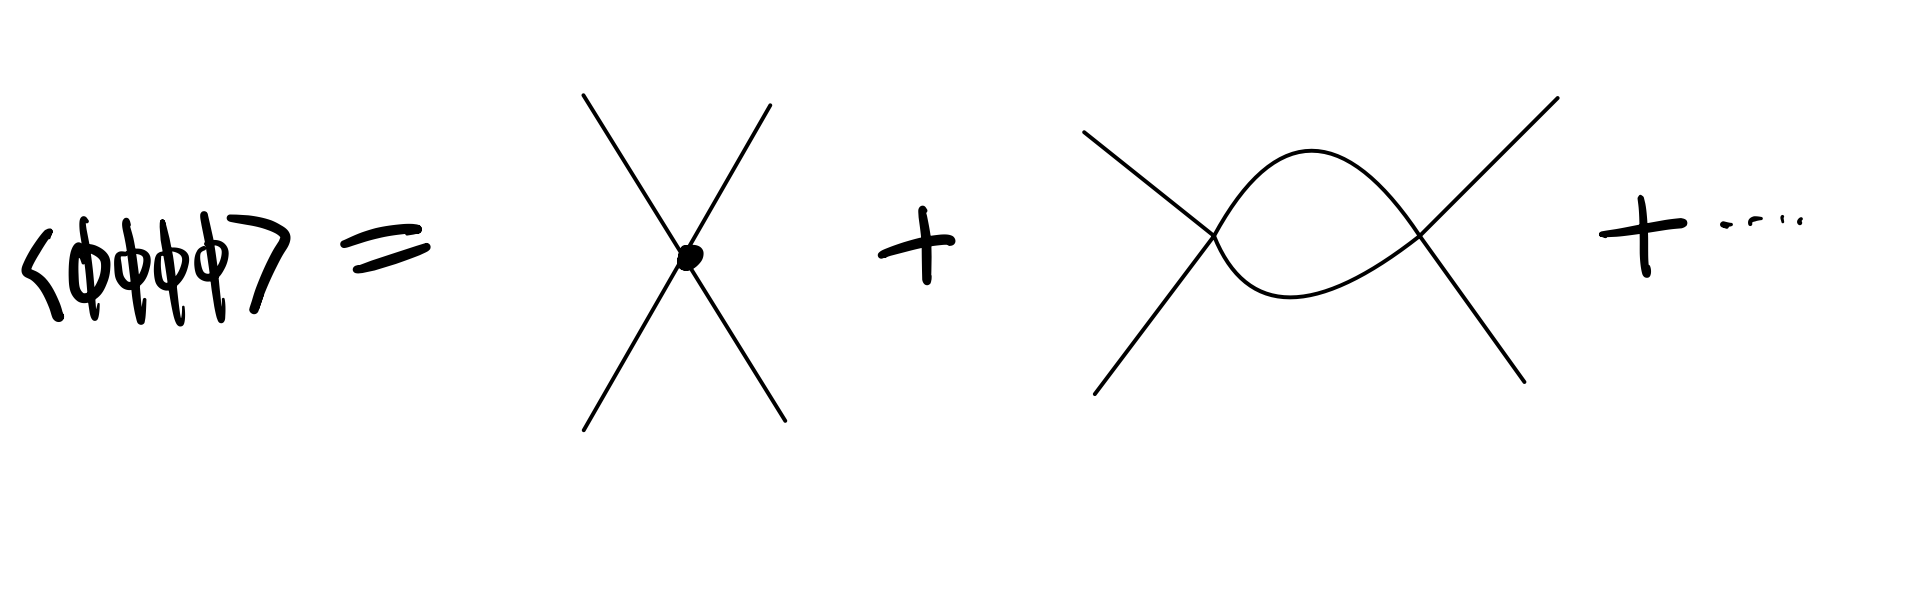
\includegraphics[scale=0.3]{Lectures/Figures/lec15-phi4observable.png}
\end{center}

Which evaluates to:
\begin{equation}
    \avg{\phi_{p_1}\phi_{p_2}\phi_{p_3}\phi_{-p_1-p_2-p_3}} = G(p_1)G(p_2)G(p_3)G(-p_1-p_2-p_3)\left[-\lambda + \left(\frac{\lambda}{4}\right)^2\int_{p'}G(p')G(p_1 + p_2 - p') + \ldots \right]
\end{equation}
Let us maximally simplify this observable - we want something that depends on a scale and not 4 different kinds of momentum. For simplicity then, we set all momenta to be equal and divide by the $GGGG$ (and set $m = 0$):
\begin{equation}
    G_4 = \frac{\avg{\phi\phi\phi\phi}}{GGGG} = -\lambda + \left(\frac{\lambda}{4}\right)^2\int_{p'}G(p')G(2p - 2p') + \ldots
\end{equation}
This measures the coupling (at leading order) and then loop corrections. The loop integral we have already done, and obtained the non-analytic piece $\log(\frac{\Lambda}{p})$. Restoring the numbers we got:
\begin{equation}
    G_4 = \lambda - \frac{3\lambda^2}{(4\pi)^2}\log(\frac{\Lambda}{p}) + \ldots
\end{equation}
why we were unhappy is because the non-analytic piece appears to blow up at high and low energies. In particular this is distressing because we found the coupling to be marginally irrelevant.

But what did we learn from RG? It showed that observables depend on a correlated way on the momenta $p$ and the coupling $\lambda$. The observables should not change if we simultaneously changes the scale (here, $p$) and the coupling in a way that respects this correlation, i.e. via the $\beta$ function. This will allow us to resum all the terms appearing in $G_4$ here that are important at weak coupling.

We study:
\begin{equation}
    0 = p\dod{}{p}G_4(p, \lambda(p)) = (p\p_p + p\dpd{\lambda}{p}\p_\lambda) G_4(p, \lambda) = (p\p_p - \beta_\lambda \p_\lambda) G_4(p, \lambda) 
\end{equation}
Thus we have the C-Z equation:
\begin{equation}
    \boxed{0 = (p\p_p - \beta_\lambda \p_\lambda) G_4(p, \lambda)}
\end{equation}
Writing this in terms of $\tau = \log \frac{p}{m}$ then:
\begin{equation}
    (\p_\tau - \beta\lambda \p_\lambda)G_4(\tau, \lambda) = 0
\end{equation}
If $\beta_\lambda$ is a constant than we just have:
\begin{equation}
    (\p_\tau - \beta \p_\lambda)G_4(\tau, \lambda) \implies G_4(\tau, \lambda) = f(\beta\tau + \lambda)
\end{equation}
i.e. a wave solution whose profile can be constrained with $G_4(0, \lambda)$. But of course here $\beta$ is not a constant, but it is not much more complicated. With $\beta_\lambda = \alpha\lambda^2$, we have:
\begin{equation}
    0 = (\p_\tau - \alpha\lambda^2\p_\lambda)G_4(\tau, \lambda)
\end{equation}
now taking $\frac{d\lambda}{\lambda^2} = dg$ so $g = -\frac{1}{\alpha\lambda}$:
\begin{equation}
    0 = (\p_\tau - \p_g)G_4(\tau, g)
\end{equation}
therefore:
\begin{equation}
    G_4(p, \lambda) = f(\tau + g) = f(\log(\frac{p}{m}) - \frac{1}{\alpha\lambda})
\end{equation}
Now we use perturbation theory to match what this observable is (RG and PT complement each other). From PT:
\begin{equation}
    G_4(m, \lambda) = -\lambda + \ldots = f(-\frac{1}{\alpha\lambda})
\end{equation}
Thus to leading order:
\begin{equation}
    f(x) = \frac{1}{\alpha x}
\end{equation}
Therefore:
\begin{equation}
    G_4(p, \lambda) = \frac{1}{\alpha}\frac{1}{\log(\frac{p}{m}) - \frac{1}{\alpha\lambda}} = -\frac{\lambda}{1 - \alpha\lambda\log(\frac{p}{m})} = -\frac{\lambda}{1 - \frac{3\lambda}{(4\pi)^2}\log(\frac{p}{m})}
\end{equation}
This looks like we resummed a bunch of higher order terms (in $\lambda \log p)$. Indeed if we expanded it then we would recover our PT expansion. As $p \to 0$, the denominator goes to infinity and thus the effective coupling goes to zero at low energies, as we found in RG. If $p$ increases, we get a Landau pole in the above expression at $p = me^{\frac{1}{\alpha\lambda}}$, i.e. we lose control over the theory. Note that in QCD where the coupling is marginally relevant, when $\beta_\lambda < 0$ ($\alpha < 0$) we get the opposite; we have a breakdown as $p$ decreases, and there is a critical energy scale $p = me^{-\frac{1}{\abs{\alpha}\lambda}}$ at this breakdown. Here we get confinement and symmetry breaking. In the BCS theory, we get a superconductor.

The conclusion of this all is; in RG we say that couplings ``run'', and this defines the energy scales in which we have control over the theory.

You are encouraged to read the chapter in Peskin - it presents the more general version.
\newpage
\section{Scattering and the LSZ Reduction Formula}

\subsection{Motivation}
We've focused on correlation functions to relate our theories to experiments. Now, we see how correlators enter into scattering - one of our most direct probes of nature.

Smashing things together can tell us a lot about systems; for example it can reveal the shape of composite particles, e.g. Rutherford scattering of electrons off of a nucleus. 

\begin{center}
    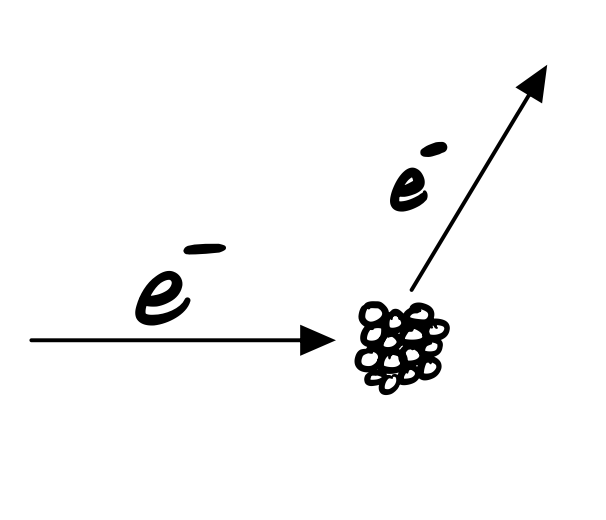
\includegraphics[scale=0.3]{Lectures/Figures/lec16-rutherford.png}
\end{center}

We can also probe the structure of interactions, e.g. a collision between an electron and proton, and even learn about the presence of other particles if we observe that there is energy missing/the scattering appears ``inelastic'' (e.g. on the left we have an elastic collision, on the right we have a collision that appears inelastic as at high enough energy, an unstable pion that decays into two photons is produced, and we didn't keep track of the energy of these).

\begin{center}
    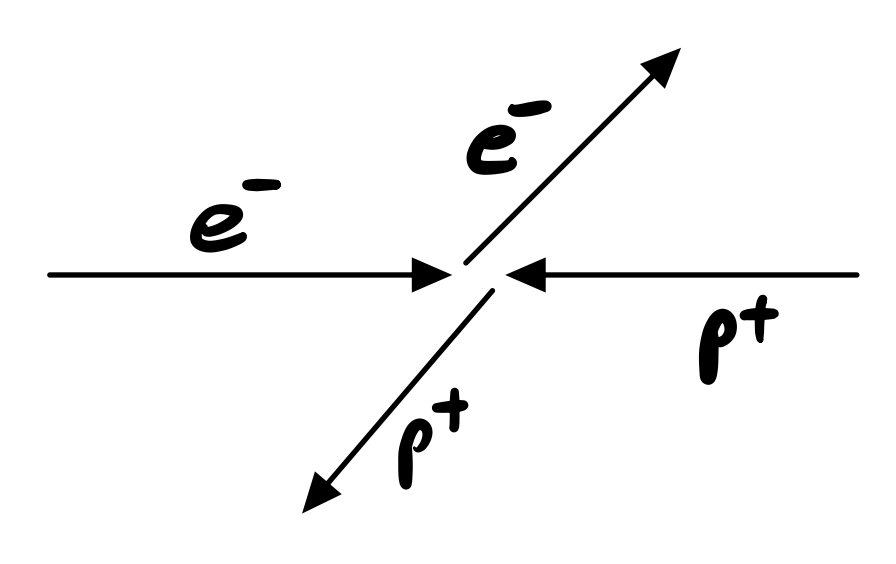
\includegraphics[scale=0.3]{Lectures/Figures/lec16-elasticcollision.png}
    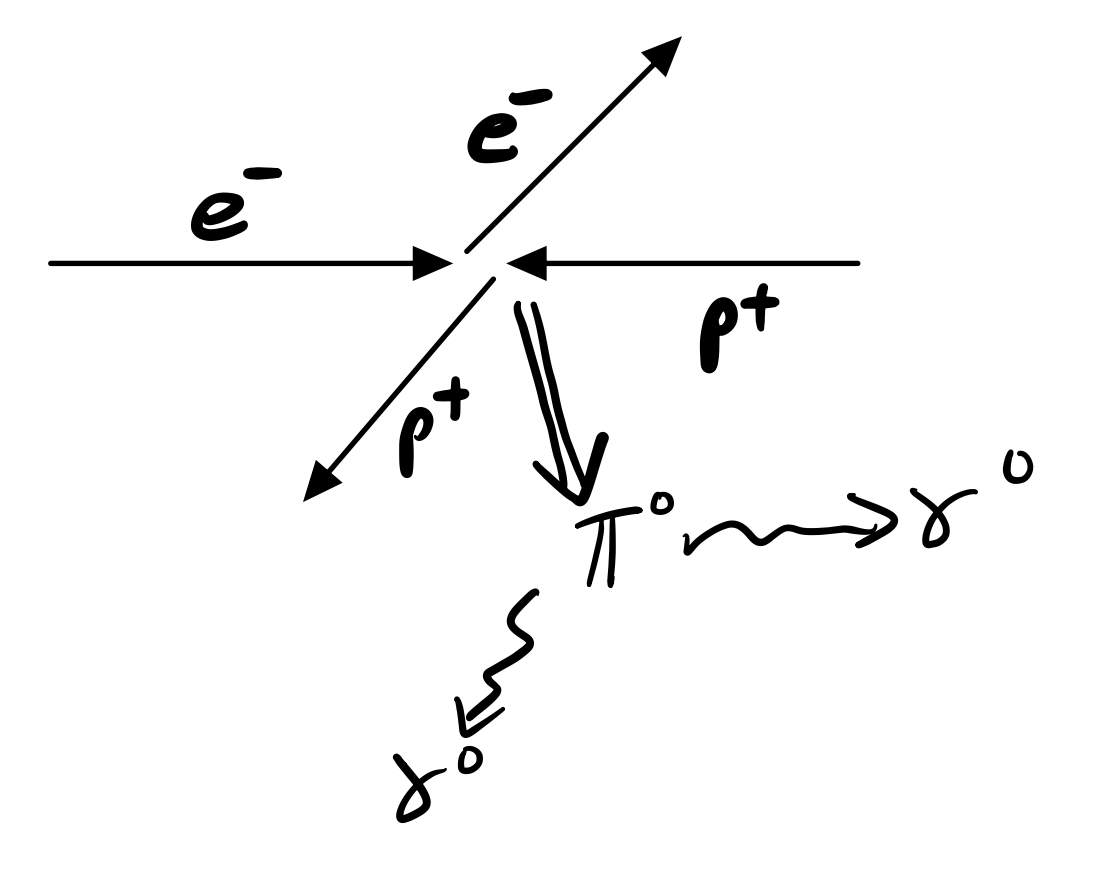
\includegraphics[scale=0.3]{Lectures/Figures/lec16-inelasticcollision.png}
\end{center}

What can we say about scattering states? Clearly, they have nontrivial time evolution and thus are not eigenstates. But, at $t \to -\infty$, they look like a collection of single-particle eigenstates. Let's take that as our starting point.

\subsection{Trivial time-evolution of free theories}

Recall single particle states for a free QFT. There, we have:
\begin{equation}
    \ket{\v{k}} = \hat{a}^\dag_{\v{k}}\ket{0}
\end{equation}
with the Lorentz-covariant normalization:
\begin{equation}
    \braket{\v{k}}{\v{k}'} = 2\e_\v{k}(2\pi)^d\delta^d(\v{k} - \v{k}')
\end{equation}
with dispersion $\e_\v{k} = \sqrt{\v{k}^2 + m^2}$. The raising/lowering operators we could wwrite in terms of the fields and their conjugate momenta:
\begin{equation}
    \begin{split}
        \hat{a}_\v{k} &= \e_\v{k}\hat{\phi}_\v{k} + i\hat{\pi}_\v{k} = \e_\v{k}\hat{\phi}_\v{k} + i\p_t\hat{\phi}_\v{k}
        \\ \hat{a}_\v{k}^\dag &= \e_\v{k}\hat{\phi}_{-\v{k}} - i\hat{\pi}_{-\v{k}} = \e_\v{k}\hat{\phi}_{-\v{k}} - i\p_t\hat{\phi}_{-\v{k}}
    \end{split}
\end{equation}
Thus, we can write the field operator as:
\begin{equation}
    \hat{\phi}_\v{k} = \frac{1}{2}(\hat{a}_\v{k} + \hat{a}^\dag_{-\v{k}})
\end{equation}
and this choice of basis was conveneint at it diagonalized the Hamiltonian, with:
\begin{equation}
    [\hat{H}, \hat{a}_\v{k}^\dag] = \e_\v{k}\hat{a}^\dag_\v{k}
\end{equation}
Studying the time-dependence:
\begin{equation}
    \begin{split}
        \hat{\phi}_\v{k}(t) &= \frac{1}{2\e_\v{k}}e^{i\hat{H}t}(\hat{a}_\v{k} + \hat{a}^\dag_{-\v{k}})e^{-i\hat{H}t}
        \\ &= \frac{1}{2\e_\v{k}}(e^{-i\e_\v{k}t}a_\v{k} + e^{i\e_\v{k}t}a_{-\v{k}}^\dag)
    \end{split}
\end{equation}
and:
\begin{equation}
    \p_t \hat{\phi}_\v{k}(t) = \frac{i}{2}(e^{-i\e_\v{k}t}a_{\v{k}} - e^{i\e_\v{k}t}a_{-\v{k}}^\dag)
\end{equation}
Note then that:
\begin{equation}
    e^{-i\e_\v{k}t}a_\v{k} = (\e_\v{k} + i\p_t)\hat{\phi}_\v{k}(t) \implies a_\v{k} = e^{i\e_\v{k}}(\e_\v{k} + i\p_t)\hat{\phi}_\v{k}(t)
\end{equation}
is time-independent. The $\hat{a}_\v{k}$ creates a single particle state. We can create 2-particle (and more) states by acting via multiple raising operators $\ket{\v{k}_1 \ldots \v{k}_n} = a_{\v{k}_1}^\dag \ldots a_{\v{k}_n}^\dag\ket{0}$ but not much will happen in a free theory, the time dependence is trivial.

\subsection{Interacting theories - In/Out states and the S-Matrix}
The fact that the above expression for $\hat{a}_\v{k}$ was time-independent relied on the fact that $[\hat{H}, \hat{a}_\v{k}] = -\e_\v{k}\hat{a}_\v{k}$. But, with interactions the Hamiltonian generally has more terms than just the quadratic $\hat{a}^\dag\hat{a}$ term, and could have quartic (or higher) interactions. So, this time-independent expression does not generically hold; instead, they are time-dependent. However, we can still consider the expressions:
\begin{equation}
    \begin{split}
        a_\v{k}(t) &= e^{i\e_\v{k}}(\e_\v{k} + i\p_t)\hat{\phi}_\v{k}(t)
        \\ a_\v{k}^\dag(t) &= e^{-i\e_\v{k}}(\e_\v{k} - i\p_t)\hat{\phi}_{-\v{k}}(t)
    \end{split}
\end{equation}
Which we note are \emph{not} equal to the Heisenberg evolved operators $e^{i\hat{H}t}\hat{a}e^{-i\hat{H}t}$ in the interacting theory, as there will now be additional commutations of $\hat{a}$ with $\hat{H}$.

A guess for what creates a 2-particle state at asymptotically early times is:
\begin{equation}
    \ket{i} = a_{\v{k}_1}^\dag(t=-\infty)a_{\v{k}_2}^\dag(t=-\infty)\ket{0}
\end{equation}
i.e. we assume that in the infinite past, we just have these simple 2-particle states as we did in the free theory. The intuition for this is far-separated wavepackets do not interact. Note that however these are not 2-particle eigenstates in the interacting theory. But this is OK. All that we need for this to work is for objects like $a^\dag_{\v{k}_1}(-\infty)\ket{0}$ to have some overlap with the true single-particle eigenstates of the interacting Hamiltonian/theory, $\bra{\v{k}}$. I.e. we want:
\begin{equation}
    \bra{\v{k}}a^\dag_{\v{k}'}\ket{0} = C\delta^d(\v{k} - \v{k}')
\end{equation}
Note that we can't solve the interacting theory fully, but we do rely on the assumption that theories with a mass gap have well-defined single-particle excitations. Also note that the fact that the above overlap is proportional to a delta function follows by spatial translation symmetry.

So, we have a candidate for the ``in'' states to scattering. Now, let's consider the ``out'' states. Even though there may be very very complicated dynamics and states at intermediate times, the ``out'' states can be assumed to also be very simple at late times:
\begin{equation}
    \ket{f} = a^\dag_{\v{k}_1'}(t=+\infty)a^\dag_{\v{k}_2'}(t=+\infty)\ket{0}
\end{equation}
Note that if we reverse time evolve an out state back to very early times we will have something that looks very complicated (and same for the in states - if we time evolve it it will be a complicated linear combination of out states). Note also - we consider exact $\v{k}$ states here, in reality Heisenberg uncertainty tells us that we should consider smeared wavepackets. It doesn't change the discussion that much, so for our discussion here we ignore it (but if you read Srednicki, you will see the smearing go along for the ride there).

The ``S-Matrix'' is the amplitude for a specific ``in'' state $\ket{i}$ to, after time evolution, produce a given out state $\ket{f}$:
\begin{equation}
    S_{fi} = \braket{f}{i}
\end{equation}
with:
\begin{equation}
    p(i \to f) = \abs{\braket{f}{i}}^2
\end{equation}
One might worry that there doesn't appear to be time-evolution appearing in the above expression (we take the direct overlap of $\ket{i}$ and $\ket{f}$), but the time-evolution is in some sense accounted for in $\ket{f}$, and this definition of the matrix elements does indeed give the relevant amplitudes.

\subsection{2-to-2 S-matrix and LSZ formula}
Consider the matrix elements for a 2 particle to 2 particle scattering:
\begin{equation}
    \braket{f}{i} = \bra{0}\hat{a}_{\v{k}_1'}(\infty)\hat{a}_{\v{k}_2'}(\infty)\hat{a}_{\v{k}_1}(-\infty)\hat{a}_{\v{k}_2}(-\infty)\ket{0}
\end{equation}
We start by finding a formula for the difference $\hat{a}_\v{k}^\dag(\infty) - \hat{a}_\v{k}^\dag(-\infty)$, which would vanish in the free theory.

We write the difference as an integral over time:
\begin{equation}
    \begin{split}
        \hat{a}^\dag_\v{k}(\infty) - \hat{a}_\v{k}^\dag(-\infty) &= \int_{-\infty}^\infty dt \p_t \hat{a}^\dag_\v{k}(t) 
        \\ &= \int_{-\infty}^\infty dt \p_t\left[e^{-i\e_\v{k}t}(\e_\v{k} - i\p_t)\hat{\phi}_{-\v{k}}(t)\right]
        \\ &=\int dt e^{-i\e_\v{k}t}(-i\e_\v{k} + \p_t)(-i)(i\e_\v{k} + \p_t)\hat{\phi}_{-\v{k}}(t)
        \\ &= -i\int dt e^{-i\e_\v{k}t}(\p_t^2 + k^2 + m^2)\hat{\phi}_{-\v{k}}(t)
    \end{split}
\end{equation}
Now plugging in the Fourier transform of the $\hat{\phi}_{-\v{k}}  \int d^dx e^{i\v{k} \cdot \v{x}}\hat{\phi}(t, \v{x})$:
\begin{equation}
    \hat{a}^\dag_\v{k}(\infty) - \hat{a}_\v{k}^\dag(-\infty) = -i\int d^{d+1}x e^{-i\e_\v{k}t + i\v{k} \cdot \v{x}}(\p_t^2 + k^2 + m^2)\hat{\phi}(t, \v{x})
\end{equation}
Now, we observe that the $k^2$ is the same thing as the $-\nabla^2$ acting on the left (brings down two factors of $(i\v{k})$). By twicefold integration by parts, we can make it act on the right, and so:
\begin{equation}
    \hat{a}^\dag_\v{k}(\infty) - \hat{a}_\v{k}^\dag(-\infty) = -i\int d^{d+1}x e^{-i\e_\v{k}t + i\v{k} \cdot \v{x}}\left(\p_t^2 - \nabla^2 + m^2\right)\hat{\phi}(t, \v{x})
\end{equation}
Thus:
\begin{equation}
    \boxed{\hat{a}^\dag_\v{k}(\infty) - \hat{a}_\v{k}^\dag(-\infty) = -i\int d^{d+1}x e^{ik_\mu k^\mu}(m^2 - \p^2)\hat{\phi}(t, \v{x})}
\end{equation}
with $k_\mu = (-\e_\v{k}, \v{k})$. We notice that the $\p^2 - m^2$ operator is just the Klein-Gordon operator, for which $(\p^2-m^2)\phi = 0$ in a free theory, as we said it would. But it does \emph{not} vanish in an interacting theory. For example with $\mathcal{L}_{\text{int}} = \frac{1}{3}\lambda \phi^3$ we would get something like:
\begin{equation}
    (\p^2 - m^2)\phi = \lambda \phi^2 \neq 0
\end{equation}

The expression we derived looks somewhat complicated, but it will eventually simplify a lot, when we plug it into our expression into $\braket{f}{i}$. Before doing so, we add in the time-ordering symbol for free:
\begin{equation}
    \braket{f}{i} = \bra{0}\mathcal{T}\{\hat{a}_{\v{k}_1'}(\infty)\hat{a}_{\v{k}_2'}(\infty)\hat{a}_{\v{k}_1}(-\infty)\hat{a}_{\v{k}_2}(-\infty)\}\ket{0}
\end{equation}
Then, using what we have derived for the difference, we can write:
\begin{equation}
    \begin{split}
        \hat{a}^\dag_{\v{k}_1}(-\infty) = a_{\v{k}_1}^\dag(\infty) + i\int_{x_1}e^{ik_1x_1}(m^2 - \p_{x_1}^2)\phi(x_1)
        \\ \hat{a}_{\v{k}'_1}(\infty) = a_{\v{k}_1}(-\infty) + i\int_{x_1'}e^{-ik_1x_1'}(m^2 - \p_{x_1'}^2)\phi(x_1')
    \end{split}
\end{equation}
Thanks to the time-ordering (which interachanges the order of things such that we get annihilations of the vaccum via $a\ket{0} = 0$ and $\bra{0}a^\dag = 0$), we end up with:
\begin{equation}
    \boxed{\braket{f}{i} = i^4\int_{x_1x_2x_1'x_2'}e^{ik_1x_1}e^{ik_2x_2}e^{-ik_1'x_1'}e^{-ik_2'x_2'}(m^2 - \p_{x_1}^2)(m^2 - \p_{x_2}^2)(m^2 - \p_{x_1'}^2)(m^2 - \p_{x_2'}^2)\bra{0}\mathcal{T}\{\hat{\phi}(x_1)\hat{\phi}(x_2)\hat{\phi}(x_1')\hat{\phi}(x_2')\}\ket{0}}
\end{equation}
This is the LSZ-formula for 2-to-2 scattering. But it can be easily generalized to $n$-to-$n'$ (see Srednicki Eq. (5.15) - there we see that we get a $n + n'$-point function). But the most experimentally relevant ones will be $2$-to-$n'$.

The key takeaway is that the S-matrix is basically made up of time-ordered correlators.

\subsection{2 Comments - Normalization and (No) Multiple Particles}
There is one slight subtlety here. In an interacting theory, we generically expect that our normalization coefficient $C$ will not be unity;
\begin{equation}
    \bra{\v{k}}a_{\v{k}'}^\dag\ket{0} = C\delta(\v{k} - \v{k}')
\end{equation}
Said differently:
\begin{equation}
    \bra{\v{k}}\hat{\phi}(\v{x})\ket{0} = \bra{\v{k}}e^{i\v{P} \cdot \v{x}}\phi(0)e^{-i\v{P}\cdot\v{x}}\ket{0} = e^{i\v{k}\cdot\v{x}}\bra{\v{k}}\phi(0)\ket{0}
\end{equation}
The $\bra{\v{k}}\phi(0)\ket{0}$ is a Lorentz scalar, and the $k$-dependence can only enter through $k^2 = -m^2$. Thus it depends on the parameters of the theory $(\lambda, \lambda', m^2, \ldots)$. For free theory, $\bra{\v{k}}\phi(0)\ket{0} = 1$. We will now rescale $\hat{\phi}$ such that it is equal to one. In practice, this is accomplished via adding $-\frac{1}{2}\delta Z\int (\p\phi)^2$ to the Lagrangian.

Furthermore, one can check that $a^\dag_{\v{k}}(-\infty)$ does \emph{not} create multi-particle states (at asymptotically early times). The detailed argument is given in Srednicki Section 5 (read it!) but here we give the intuition. Namely, it does not have the correct energy to create multiple particles - this observation crucially relies on a mass gap, or separation between single-particle states and the rest of the spectrum, as is sketched below:

\begin{center}
    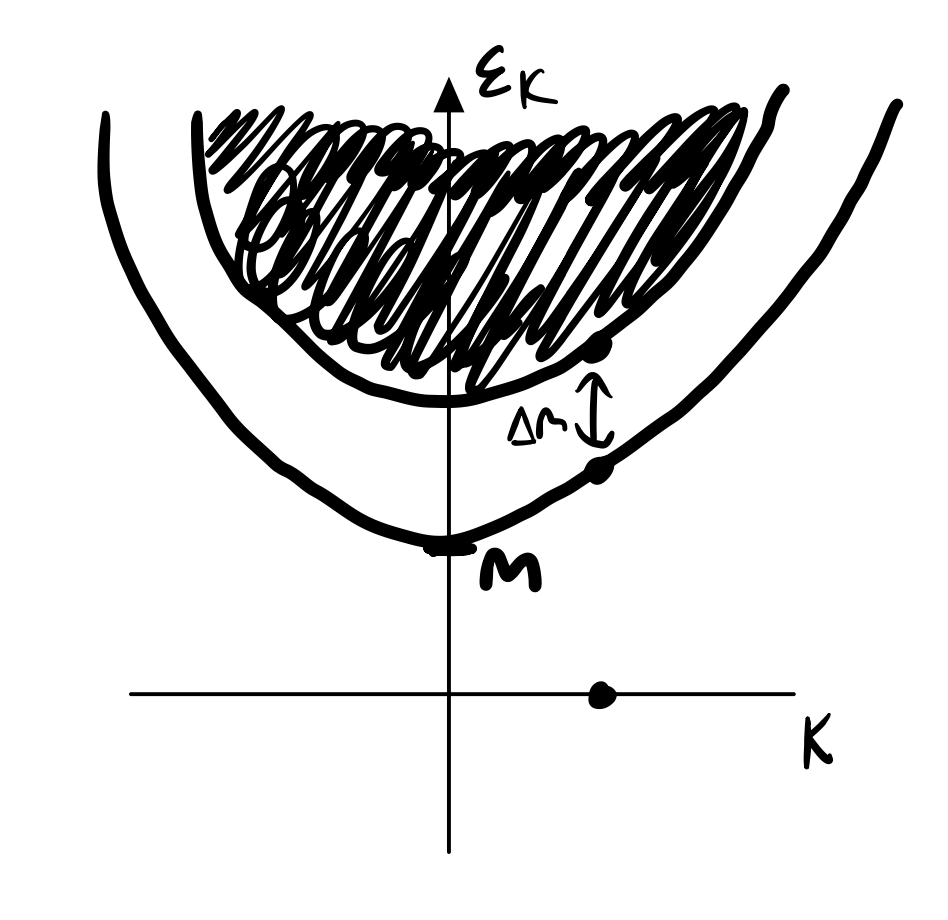
\includegraphics[scale=0.3]{Lectures/Figures/lec16-massgap.png}
\end{center}

This tells us that it is not possible for define the S-matrix for massless/gapless theories. Unfortunately, this contains QFTs that we see in nature, including Conformal Field Theories/CFTs. These issues can be tackled in QED using techniques of soft divergence. But for strongly interacting gapless theories, we can't distinguish single-particle states from a soup of dressed multiple particles, and there is no hope for the S-matrix.
\newpage
\section{S-matrix elements}
\emph{Note: I was unable to make it to this lecture due to travel constraints, so these notes are adapted from Inci's lecture notes - many thanks!}

\subsection{Review of the LSZ Formula}
Before the break, we discussed the LSZ formula, which allowed us to convert observables (specifically, time-ordered correlators) into S-matrices (i.e. scattering/transition amplitudes).

In more detail, recall that the $S$-matrix consists of amplitudes $\braket{f}{i}$ for a specific in state, e.g. $\ket{i} = a^\dag_{\v{k}_1}(-\infty)a^\dag_{\v{k}_2}(-\infty)\ket{0}$ to evolve into a specific out state, e.g. $\bra{f} = \bra{0}a_{\v{k}_1'}(\infty)a_{\v{k}_2'}(\infty)$. The LSZ formula relates this matrix element to a time-ordered correlator:
\begin{equation}
    \braket{f}{i} = i^4\int_{x_1, x_2, x_1', x_2'}e^{i(k_1x_1 + k_2x_2 - k_1'x_1' - k_2'x_2')}(m^2 - \p_1^2)(m^2 - \p_2^2)(m^2 - \p_{1'}^2)(m^2 - \p_{2'}^2)\bra{0}\mathcal{T}\set{\phi(x_1)\phi(x_2)\phi(x_1')\phi(x_2')}\ket{0}
\end{equation}
Note that the $k_i$ appearing in the above are 4-momenta, with the $k_i^0$/energy being fixed by the spatial momentum:
\begin{equation}
    k_i^0 = \e_{\v{k}_i} = \sqrt{m^2 + \v{k}_i^2}
\end{equation}
The S-matrix is thus an ``on-shell'' observable.

We also note that in order for the normalization to be correct (in interacting theories $\bra{\v{k}}a_{\v{k}'}^\dag(-\infty)\ket{0} = C\delta(\v{k} - \v{k'})$ with $C$ not necessarily 1), we normalize the fields such that $\bra{\v{k}}\phi(0)\ket{0} = 0$, so:
\begin{equation}
    \bra{\v{k}}\phi(x)\ket{0} = e^{ikx}\bra{k}\phi(0)\ket{0} = e^{ikx}
\end{equation}

\subsection{S-matrix for interacting scalar QFT}
We consider the Lagrangian:
\begin{equation}
    \mathcal{L} = -\frac{1}{2}(\p\phi)^2 - \frac{1}{2}m^2\phi^2 - \frac{1}{3!}g\phi^3 - \frac{1}{4!}\lambda\phi^4
\end{equation}
Integrating the LSZ formula by parts twice, we obtain the expression:

\begin{equation}
    \bra{f}{i} = (m^2 + k_1^2)(m^2 + k_2^2)(m^2 + k_1'^2)(m^2 + k_2'^2)\int_{x_1, x_2, x_1', x_2'}e^{ik_1x_1 + k_2x_2 - k_1x_1' - k_2x_2'}\avg{\phi(x_1)\phi(x_2)\phi(x_1')\phi(x_2')}
\end{equation}
where we have the time ordered correlator:
\begin{equation}
    \begin{split}
        \avg{\phi(x_1)\phi(x_2)\phi(x_1')\phi(x_2')} &\equiv \avg{\phi(x_1)\phi(x_2)\phi(x_1')\phi(x_2')}_C 
        + \avg{\phi(x_1)\phi(x_1')}\avg{\phi(x_2)\phi(x_2')} 
        \\ &+ \avg{\phi(x_1)\phi(x_2')}\avg{\phi(x_2)\phi(x_1')} + \avg{\phi(x_1)\phi(x_2)}\avg{\phi(x_1')\phi(x_2')} 
    \end{split}
\end{equation}
Note that since $k_1, k_2, k_1', k_2'$ make up our ``on-shell'' 4-point function, it seems like the $m^2 + k_i^2$ gives zero, but the connected part will always have $G(k_1)G(k_2)G(k_1')G(k_2')$ which cancels out the zeroes.

\subsection{Disconnected Terms and the Free-Field S-Matrix}
We look at the disconnected terms in the above matrix element. The first is:
\begin{equation}
    (1) = \int_{x_1, x_2, x_1' x_2'}e^{i(k_1x_1 + k_2x_2 - k_1'x_1' - k_2'x_2')}G(x_1' - x_1) G_2(x_2' - x_2)
\end{equation}
with $G(x) = G_F(x) = \bra{0}\mathcal{T}\set{\phi(x)\phi(0)}\ket{0}$. Defining $\tilde{x}_i = x_i' - x_i$ we have:
\begin{equation}
    (1) = \int_{x_1, x_2, x_1', x_2'}e^{ix_1(k_1 - k_1')}e^{ix_2(k_2 - k_2')}e^{-ik_1'\tilde{x}_1}G(\tilde{x}_1)e^{-ik_2'\tilde{x}_2}G(\tilde{x}_2) = G(k_1')G(k_2')(2\pi)^{d+1}\delta^{d+1}(k_1-k_1')(2\pi)^{d+1}\delta^{d+1}(k_2 - k_2'
    )
\end{equation}
where in the second equality we Fourier transform the $e^{-ik_i'\tilde{x}_i}G(\tilde{x}_i)$s. Thus we have the nonzero term represented by the diagram:

\begin{center}
    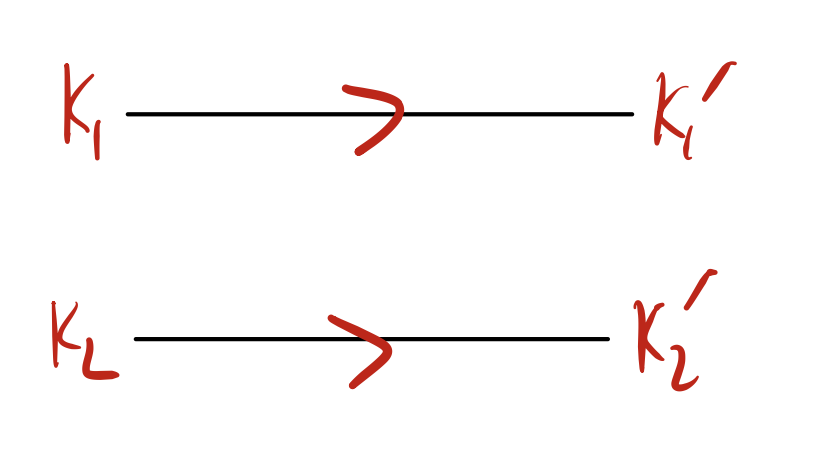
\includegraphics[scale=0.35]{Lectures/Figures/lec17-stay.png}
\end{center}

For the second disconnected term, we can follow the same procedure and obtain:
\begin{equation}
    (2) = G(k_1)G(k_2)(2\pi)^{d+1}\delta^{d+1}(k_1 - k_2')(2\pi)^{D+1}\delta^{d+1}(k_2 - k_1')
\end{equation}
which is represented by the diagram:

\begin{center}
    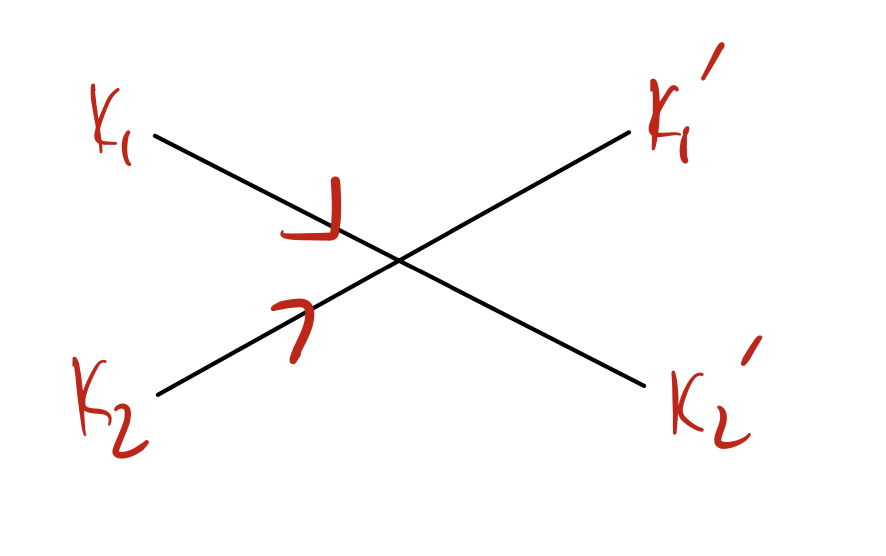
\includegraphics[scale=0.35]{Lectures/Figures/lec17-swap.png}
\end{center}

Technically, there is also a third term with $\delta^{d+1}(k_1 + k_2)$. But, this term is associated with two physical momenta/particles, i.e. $k_1^0, k_2^0 > 0$ and hence vanishes, with $\delta^{d+1}(k_1 + k_2) = 0$.

In the free theory, this would be it! We would have:
\begin{equation}
    \bra{0}a_{k_1'}a_{k_2'}a^\dag_{k_1}a^\dag_{k_2}\ket{0} = 2\e_{k_1}\e_{k_2}(2\pi)^{2(d+1)}\left[\delta^d(\v{k}_1 - \v{k}_1')\delta^d(\v{k}_2 - \v{k}_2') + \delta^d(\v{k}_1 - \v{k}_2')\delta^d(\v{k}_2 - \v{k}_1')\right]
\end{equation}
and thus obtain $\braket{f}{i} = \delta_{if}$, i.e. the $S$ matrix is the identity:
\begin{equation}
    S = 1
\end{equation}
This makes physical sense; in the free theory there is no interaction/scattering process between the particles, so all that can happen is the initial state stays the same to the final state.

\subsection{First-Order connected Term}
In an arbitrary interacting theory, we isolate the non-trivial scattering part of the $S$-matrix by writing:
\begin{equation}
    \braket{f}{i} = \delta_{if} + T_{if}
\end{equation}
or $S = 1 + iT$. The $T$ represents the non-trivial part. For the interacting scalar QFT we have written, this term looks like:
\begin{equation}
    T_{if} = (m^2 + k_1^2)(m^2 + k_2^2)(m^2 + k_1'^2)(m^2 + k_2'^2)\int_{x_1, x_2, x_1', x_2'}e^{ik_1x_1 + k_2x_2 - k_1x_1' - k_2x_2'}\avg{\phi(x_1)\phi(x_2)\phi(x_1')\phi(x_2')}_C
\end{equation}
where we have subtracted off the free field theory contribution.

Let us evaluate this. We use translation invariance of the theory to simplify our life, substituting $x_1 \to x_1 + x_2'$, $x_2 \to x_2 + x_2'$, $x_1' \to x_1' + x_2'$. We then have:
\begin{equation}
    \avg{\phi(x_1)\phi(x_2)\phi(x_1')\phi(x_2')}_C = \avg{\phi(x_1 - x_2')\phi(x_2-x_2')\phi(x_1-x_2')\phi(0)}_C \equiv \avg{\phi(x_1)\phi(x_2)\phi(x_1')\phi(0)}_C 
\end{equation}
where in the last equality we use our new renamed variables.
Thus:
\begin{equation}
    T_{if} = (m^2 + k_1^2)(m^2 + k_2^2)(m^2 + k_1'^2)(m^2 + k_2'^2)\int_{x_1, x_2, x_1', x_2'}e^{ik_1x_1 + k_2x_2 - k_1x_1' - k_2x_2'}\avg{\phi(x_1)\phi(x_2)\phi(x_1')\phi(0)}_C = (2\pi)^{d+1}\delta^{d+1}(k_1 + k_2 - k_1' - k_2')i\mathcal{M}.
\end{equation}
Where in the last equality we Fourier transform and define  $\mathcal{M}$ as the matrix element, with:
\begin{equation}
    i\mathcal{M} = (m^2 + k_1^2)(m^2 + k_2^2)(m^2 + k_1'^2)(m^2 + k_2'^2)\avg{\phi_{k_1}\phi_{k_2}\phi_{-k_1'}\phi(0)}_C
\end{equation}
with $\phi_{k_i} = \int_{x_i}e^{i x_ik_i}\phi(x_i)$. As usual. For the free theory,$\avg{\phi_{k_1}\phi_{k_2}\phi_{-k_1'}\phi(0)}_C = 0$ and $\mathcal{M}$ vanishes.

Let us compute the matrix element to leading order in the coupling; there is no $O(g)$ contribution at this order, but we will find a $O(\lambda)$ contribution:
\begin{equation}
    \avg{\phi_{k_1}\phi_{k_2}\phi_{-k_1'}\phi(0)}_C \sim \avg{\phi_{k_1}\phi_{k_2}\phi_{-k_1'}\phi(0)\left(\frac{-i}{4!}\lambda \int_x \phi^4(x)\right)}_{g,\lambda = 0}
\end{equation}
There are $4 \cdot 3 \cdot 2 \cdot 1 = 4!$ ways of ordering the fields/choices for Wick contractions, which cancels out with the $\frac{1}{4!}$ present in the interaction term of the Lagrangian.

Looking at the types of contractions, we have:
\begin{equation}
    \wick{\c1 \phi(x) \c1 \phi(0)} = G(x)
\end{equation}
\begin{equation}
    \wick{\c1 \phi(x) \c1 \phi_k} = \int_{x'}e^{ikx'}\wick{\c1 \phi(x) \c1 \phi(x')} = \int_{x'}G(x' - x) \stackrel{\tilde{x} = x' - x}{=} e^{ikx}\int_{\tilde{x}} e^{ik\tilde{x}}G(\tilde{x}) = e^{ikx}G(k)
\end{equation}
Thus:
\begin{equation}
    \begin{split}
        \avg{\phi_{k_1}\phi_{k_2}\phi_{-k_1'}\phi(0)}_C = -i\lambda\int_{x}e^{i(k_1 + k_2 - k_1')x}G(k_1)G(k_2)G(k_1')G(x) &= -i\lambda G(k_1)G(k_2)G(k_1')G(k_1 + k_2 - k_1') 
        \\ &= -i\lambda G(k_1)G(k_2)G(k_1')G(-k_2')
    \end{split}
\end{equation}
Graphically, we have the diagram:

\begin{center}
    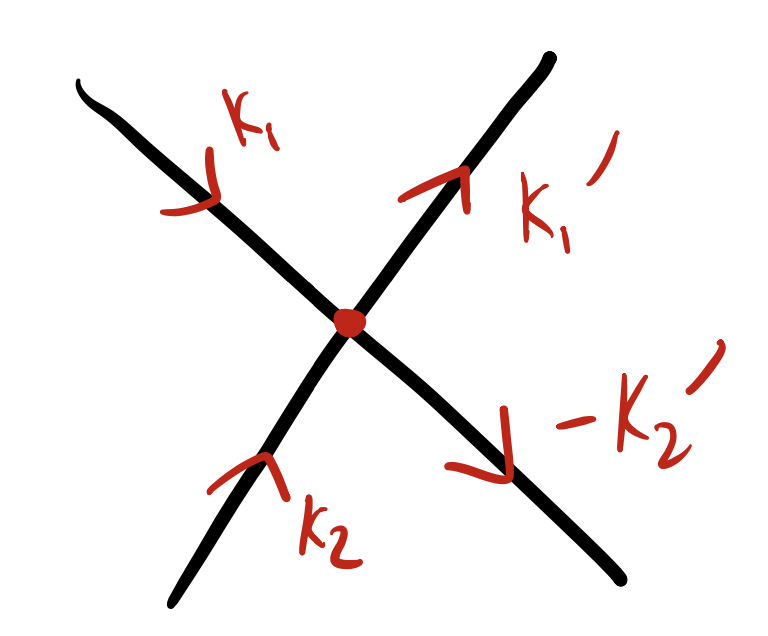
\includegraphics[scale=0.3]{Lectures/Figures/lec17-4pointvertex.png}
\end{center}

Note that all the $G(\cdot)$ cancel out the prefactors, since $G(k) = \frac{-i}{k^2 + m^2}$. Thus we find that $i\tilde{M}_{i \to f} = -i\lambda$, or that:
\begin{equation}
    \tilde{M}(\v{k}_1, \v{k}_2 \to \v{k}_1', \v{k}_2') = -\lambda
\end{equation}
Note that we have no $\v{k}$ dependence! this is the simplest $S$-matrix.

\subsection{Higher-Order S-Matrix}

If we look at $O(g^2)$, we then have $\phi^3$ terms, which result in a non-trivial $S$-matrix. Let's look at this:
\begin{equation}
    \avg{\phi_{k_1}\phi_{k_2}\phi_{-k_1'}\phi(0)}_C \cong \frac{(-i)^2}{2}\left(\frac{g}{3!}\right)^2\int_{x, y}\avg{\phi_{k_1}\phi_{k_2}\phi_{-k_1'}\phi(0)\phi^3(x)\phi^3(y)}
\end{equation}
As is now standard, we can now count all the possible Wick contractions. $\phi(0)$ can contract with either $\phi(x)$ or $\phi(y)$, of which there are 3 each, which gives $3 \cdot 2$ contractions. At least one of the $\phi(x)$ and $\phi(y)$ must contract with each other, else the diagram is disconnected - since there are 2 remaining $\phi(x)$s and 3 remaining $\phi(y)$s (or vise versa), there is another factor of $3 \cdot 2$ contractions. Together this cancells out the $\frac{1}{3!^2}$ factor on the outside. Of the remaining fields, the last $\phi(x)$ contracts with one of $\phi_{k_1}, \phi_{k_2}, \phi_{-k_1'}$ and the other two contract with the remaining $\phi(y)$s. We can classify the diagrams we get based on which of the external momenta the $\phi(x)$ gets contracted with:

\begin{itemize}
    \item If $\phi(x)$ contracts with $\phi_{k_1'}$, then we have the S-channel:
    \begin{equation}
        \equiv -g^2\int_{x, y}e^{i(k_1 + k_2)y}G(k_1)G(k_2)e^{-ik_1'x}G(k_1')G(x)G(x-y)
    \end{equation}
    \begin{center}
        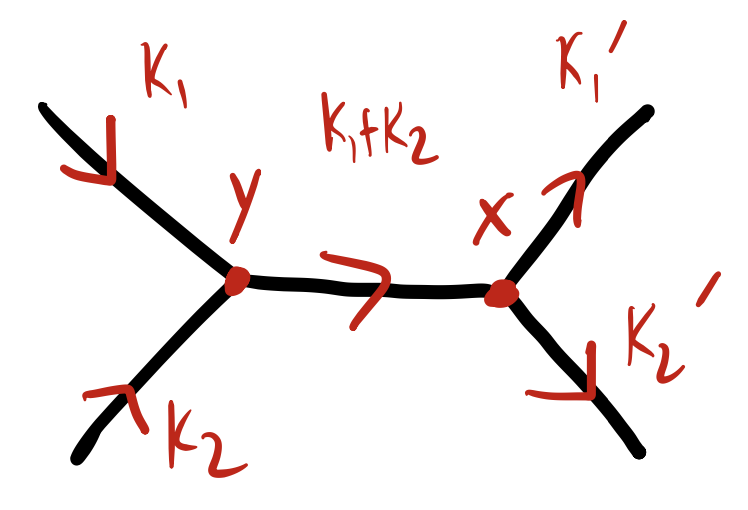
\includegraphics[scale=0.35]{Lectures/Figures/lec17-schannel.png}
    \end{center}

    \item If $\phi(x)$ contracts with $\phi_{k_1}$, then we have the u-channel:
    \begin{equation}
        \equiv -g^2\int_{x, y}e^{i(k_2 - k_1')y}e^{ik_1x}G(k_1)G(k_2)G(k_1')G(x)G(x-y)
    \end{equation}
    \begin{center}
        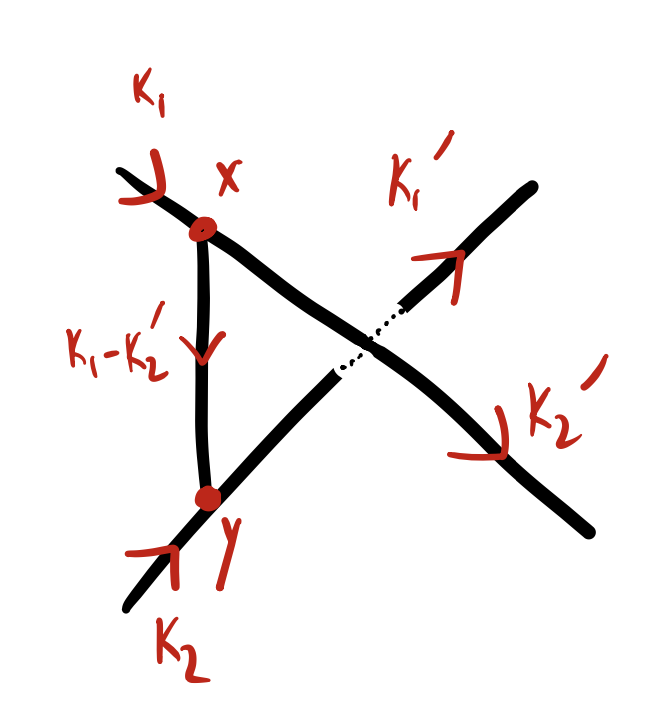
\includegraphics[scale=0.35]{Lectures/Figures/lec17-uchannel.png}
    \end{center}

    \item If $\phi(x)$ contracts with $\phi_{k_2}$, we have the t-channel:
    \begin{equation}
        \equiv -g^2\int_{x, y}e^{i(k_1 - k_1')y}G(k_1)e^{ik_2x}G(k_2)G(k_1')G(x)G(x-y)
    \end{equation}
    \begin{center}
        \includegraphics[scale=0.35]{Lectures/Figures/lec17-tchannel.png}
    \end{center}
\end{itemize}

Thus with $\tilde{y} = x - y'$, we have the matrix element:
\begin{equation}
    \begin{split}
        i\mathcal{M} &= i(m^2 + k(k_1 + k_2 - k_1')^2)(-g^2)\int_{x, \tilde{y}}e^{-ix(k_1 + k_1 - k_1')}G(x)\left[e^{-i(k_2 - k_1')\tilde{y}}G(\tilde{y}) + e^{-i(k_1 - k_1')}G(\tilde{y}) + e^{-i(k_1 + k_2)}G(\tilde{y})\right]
        \\ &= -g^2\left[G(k_1 - k_1') + G(k_1 - k_1') + G(k_1 + k_2)\right] 
        \\ &= ig^2\left[\frac{1}{m^2+ (k_2 - k_1')^2} + \frac{1}{m^2 + (k_1 - k_1')^2} + \frac{1}{m^2 + (k_1 + k_2)^2}\right]
    \end{split}
\end{equation}
\newpage
\section{Particle Cross Sections}
\subsection{Review of results + Mandelstam variables}
To summarize what we have derived thus far:
\begin{itemize}
    \item One can isolate the non-trivial part of the S-matrix as:
    \begin{equation}
        \braket{f}{i} = \delta_{if} + iT_{if}
    \end{equation}
    or $S = 1 + iT$.
    \item Translation invariance further implies that:
    \begin{equation}
        iT_{if} = (2\pi)^4\delta^4(k_1 + k_2 - k_1' - k_2')i\mathcal{M}(k_1, k_2 \to k_1', k_2')
    \end{equation}
    \item We studied $\mathcal{M}$ for two interacting theories, at tree-level:
    \begin{itemize}
        \item $\mathcal{L}_{\text{int}} = -\frac{\lambda}{4!}\phi^4$, with the diagram:
        \begin{center}
            \includegraphics[scale=0.4]{Lectures/Figures/lec18-Olambda.png}
        \end{center}
        and matrix element (independent of the momenta):
        \begin{equation}
            \mathcal{M}(k_1, k_2 \to k_1', k_2') = -\lambda
        \end{equation}
        \item $\mathcal{L}_{\text{int}} = -\frac{g}{3!}\phi^3$, with diagrams:
        \begin{center}
            \includegraphics[scale=0.4]{Lectures/Figures/lec18-Ogsquared.png}
        \end{center}
        and matrix element (dependent on the momenta):
        \begin{equation}
            \begin{split}
                \mathcal{M}(k_1. k_2 \to k_1', k_2') &= g^2\left[\frac{1}{(k_1 + k_2)^2 + m^2} + \frac{1}{(k_1 - k_1')^2 + m^2} + \frac{1}{(k_1 - k_2')^2 + m^2}\right] 
                \\ &= g^2\left[\frac{1}{m^2 - s} + \frac{1}{m^2 - t} + \frac{1}{m^2 - u}\right]
            \end{split}
        \end{equation}
        where $s, t, u$ are the \emph{Mandelstam variables}:
        \begin{equation}
            s = -(k_1 + k_2)^2, t = -(k_1 - k_1')^2, u = -(k_1 - k_2')^2
        \end{equation}
        and are the only Lorentz invariant variables that the S-matrix can depend on. Why are these the only three? First, note that the fourth momenta is fixed by the $\delta$ function, so it can depend on at most three particles. Then, further noting that $k_1^2 = k_2^2 = k_1'^2 = k_2'^2 = -m^2$, (the S-matrix is on-shell) the only way to get nontrivial variables is by taking combinations. Further, there is actually a relation between the three, so it is really only 2 that are independent:
        \begin{equation}
            s + t + u = 6m^2 - 2k_1(k_2 - k_1' - k_2') = 6m^2 - 2k_1(-k_1) = 6m^2 + 2k_1^2 = 4m^2
        \end{equation}
        where in the second equality we use the delta function. Since their sum is fixed, there are only 2 independent variables, e.g. $s, t$. But sometimes it is convenient to keep the third ($u$) around (instead of writing it as $u = 4m^2 - s - t$) as it keeps the crossing symmetry (that is, symmetry under swaps of $s/t/u$) manifest in our results.
    \end{itemize}
\end{itemize}

As an aside; here we compute the S-matrix perturbatively, but there is a research program known as the ``S-matrix bootstrap'' which is a non-perturbative approach to QFT, which essentially guesses possible matrix elements $\mathcal{M}(s, t, u)$ using all of the properties that they have to satisfy - crossing symmetry, analyticity, causality, Lorentz invariance. This program was born out of study of strongly coupled QFTs (e.g. QCD) and was abandoned for a while, but is now seeing a resurgence.

\subsection{Converting matrix elements to cross sections}
This is the last topic we will cover in this course! It is discussed in Section 10 of Srednicki, 5.1 of Schwartz, and 4.6 of Peskin. The former 2 have a slightly heuristic/faster derivation, Peskin has a slightly more careful derivation.

The cross sectional area of an object is the area $\sigma$ that we can see of an object, e.g. the 2-D ball below has a classical cross sectional area of $\sigma = 2\pi r$. 

\begin{center}
    \includegraphics[scale=0.35]{Lectures/Figures/lec18-sigma.png}
\end{center}

We can probe what $\sigma$ is by scattering objects off of it. Consider shooting a bunch of particles at an object, then the number of scattered particles in some time $T$ is given by:
\begin{equation}
    N_{\text{scatter}} = \sigma v T n
\end{equation}
where $\sigma$ is the cross section, $v$ is the speed of the particles, and $n$ is the number density. Thus:
\begin{equation}
    \sigma = \frac{N_{\text{scatter}}}{vTn}
\end{equation}
this is the classical definition of a cross section - in QM, we instead define it as the probability to scatter. Thus, in QFT the cross section is not only a measure of the size of a particle, but also how strongly it interacts.

In addition to just the cross section/total probability, we would also like to resolve the possible outgoing states. Thus, we look at the differential cross section:
\begin{equation}
    d\sigma = \frac{dP}{vT n}
\end{equation}
with $dP$ the differential probability to scatter into a state with a given $k_1', k_2'$. This formula has to be taken with a slight grain of salt, because in the thermodynamic limit ($V \to \infty$) $dP$ and $n$ both go to zero (the former because the probability for scattering into a specific momenta is zero, the latter because $n = \frac{N}{V} \to 0$). Thus, it is useful to temporarily introduce $V < \infty$, and take the density to be $n = \frac{1}{V}$ (looking at scattering off of a single-particle).

We study the differential probability:
\begin{equation}
    dP = \frac{\abs{\braket{f}{i}}^2}{\braket{i}{i}\braket{f}{f}}d\Pi; \quad d\Pi = \prod_{i=1}^n \frac{V^3 d^3k_i'}{(2\pi)^3}
\end{equation}
where $d\Pi$ accounts for a generalization to $2 \to n$ scattering. We can calibrate the normalization of this expression using the free theory (working in $D = 3 + 1$ dimensions, and for $2\to2$ scattering for simplicity):
\begin{equation}
    \braket{f}{i} = 2\e_{k_1}2\e_{k_2}(2\pi)^6\delta^3(k_1 - k_1')\delta^3(k_2 - k_2')
\end{equation}
\begin{equation}
    \braket{i}{i} = 2\e_{k_1}2\e_{k_2}(2\pi)^3\delta^3(0)\delta^3(0)
\end{equation}
\begin{equation}
    \braket{f}{f} = 2\e_{k_1'}2\e_{k_2'}(2\pi)^3\delta^3(0)\delta^3(0)
\end{equation}
Then:
\begin{equation}
    \int dP = \frac{(\delta^3(\v{k}_1 - \v{k}_1')\delta^3(\v{k}_2 - \v{k}_2'))^2}{(\delta^3(0)\delta^3(0))^2}\int d\Pi = \int\frac{(\delta^3(\v{k}_1 - \v{k}_1')\delta^3(\v{k}_2 - \v{k}_2'))^2}{(\delta^3(0)\delta^3(0))^2}\left(\frac{V}{(2\pi)^3}\right)^2 d^3k_1' d^3k_2' = \left(\frac{V}{(2\pi)^3\delta^3(0)}\right)^2 = 1
\end{equation}
So the normalization is indeed correct.

More generally for $2 \to n$:
\begin{equation}
    \braket{f}{f} = \prod_{i=1}^n 2\e_{k_i'}(2\pi)^3\delta^3(0) =  \prod_{i=1}^n 2\e_{k_i'}V
\end{equation}
\begin{equation}
    \braket{i}{i} = 2\e_{k_1}2\e_{k_2}(2\pi)^3\delta^3(0)\delta^3(0)
\end{equation}
Then looking at the overlap:
\begin{equation}
    \abs{\braket{f}{i}}^2 = (2\pi)^4\delta^4(0)(2\pi)^4\delta^3(k_1 + k_2 - \sum_{i=1}^n k_i')\abs{\mathcal{M}}^2
\end{equation}
where $(2\pi)^4\delta^4(0) = VT$. Thus looking at the differential probability:
\begin{equation}
    dP = \frac{VT(2\pi)^4\delta^4(k_1 + k_2 - \sum_{i}k_i')\abs{\mathcal{M}}^2}{2\e_{k_1}2\e_{k_2}V^2\prod_{i=1}^n(2\e_{k_i'}V)}\prod_{i=1}^n\frac{Vd^3k_i'}{(2\pi)^3} = \frac{T\abs{M}^2}{V(2\e_{k_1})(2\e_{k_2})}\left((2\pi)^4\delta^4(k_1 + k_2 - \sum_i k_i')\prod_i \frac{d^3k_i'}{(2\pi)^32\e_{k_i'}}\right)
\end{equation}
where the expression in brackets is the Lorentz-invariant phase space measure:
\begin{equation}
    d\Pi_{\text{LIPS}} = (2\pi)^4\delta^4(k_1 + k_2 - \sum_i k_i')\prod_i \frac{d^3k_i'}{(2\pi)^32\e_{k_i'}}
\end{equation}
Cross-sections are generally not Lorentz invariant, but it is nice to factor out this part that is.

Thus, returning to the differential cross section:
\begin{equation}
    d\sigma = \frac{\abs{\mathcal{M}}^2}{(2\e_{k_1})(2\e_{k_2})\abs{\v{v}_1 - \v{v}_2}}d\Pi_{\text{LIPS}}
\end{equation}
where the velocity is the group velocity:
\begin{equation}
    \v{v}_i = \dod{\e_{k_i}}{\v{k}_i} = \dod{\sqrt{\v{k}_i^2 + m^2}}{\v{k}_i} = \frac{\v{k}_i}{\e_{k_i}}
\end{equation}

We saw that $\abs{\mathcal{M}}$ was proportional to (some power of) the coupling, so as we stated previously, the cross-section is indeed a measure of the interaction.

\subsection{Evaluating 2-2 Differential Cross Section}
Lets consider a $\phi\phi \to \phi\phi$ scattering. 

\begin{center}
    \includegraphics[scale=0.35]{Lectures/Figures/lec18-scatter.png}
\end{center}

In the CoM frame, $\v{k}_1 = -\v{k}_2$ (and thus $\e_{\v{k}_1} = \e_{\v{k}_2}$). The total centre-of-mass frame energy is $E_{CM} = 2\e_{\v{k}_1}$. By momentum conservation, $\v{k}_2' = -\v{k}_1'$, and by energy conservation $2\e_{k_1} = 2\e_{k_1'}$ and so:
\begin{equation}
    \abs{\v{k}_1} = \abs{\v{k}_2} = \abs{\v{k}_1'} = \abs{\v{k}_2'}
\end{equation}
Thus the only free parameters in this problem is the norm of the momentum vector $\abs{\v{k}_1}$ and the angle of scattering $\theta$. These map to the Mandelstam variables $s$ and $t$. 

We need to put together the Lorentz-invariant phase space measure. We will see that we shall be able to remove some of the differentials.
\begin{equation}
    d\Pi_{\text{LIPS}} = (2\pi)^4\delta^4(k_1 + k_2 - k_1' - k_2')\frac{d^3k_1'}{(2\pi)^32\e_{k_1'}}\frac{d^3k_2'}{(2\pi)^32\e_{k_2'}}
\end{equation}
We can start by integrating out $\v{k}_2'$, which converts the 4-momentum conservation from the dirac delta to an energy conservation dirac delta:
\begin{equation}
    d\Pi_{\text{LIPS}} = (2\pi)\delta^4(\e_{k_1} + \e_{k_2} - \e_{k_1'} - \e_{k_2'})\frac{d^3k_1'}{(2\pi)^3(2\e_{k_1'})(2\e_{k_2'})}
\end{equation}
in the COM frame (this is a LI quantity, so we can evaluate it in any frame we like) - we go into spherical coordinates, and the the $k_1'$s appearing below are now the magnitude of the momenta:
\begin{equation}
    d\Pi_{\text{LIPS}} = (2\pi)\frac{\delta(E_{CM} - 2\e_{k_1'})}{(2\pi)^3E^2_{CM}}k_1'^2 dk_1' d\Omega
\end{equation}
The $\delta$ function fixes $\e_{k_1'} = \frac{E_{CM}}{2}$ and so fixes $k_1' = k_1$. Thus using the usual trick of the Jacobian and delta functions:
\begin{equation}
    \delta(E_{CM} - 2\e_{k_1'}) = \delta(2k_1 - 2k_1')\frac{1}{\dod{\e_{k_1'}}{k_1'}} = \frac{1}{2}\delta(k_1 -k_1')\frac{1}{v_i}
\end{equation}
Thus:
\begin{equation}
    d\Pi_{\text{LIPS}} = \frac{1}{2}\frac{1}{v_1}\frac{1}{(2\pi)^2E_{CM}^2}k_1^2d\Omega
\end{equation}
and then recalling that $v_1 = \frac{k_1}{\e_{k_1}}$, it follows that $k_1 = v_1\e_{k_1}$ and so $\e_{k_1} = v_1\frac{E_{CM}}{2}$:
\begin{equation}
    d\Pi_{\text{LIPS}} = \frac{v_1}{32\pi^2}d\Omega
\end{equation}
which is our result for the measure. It is dimensionless as it should be. It is not manifestly Lorentz invariant (an artifact of choosing a reference frame to evaluate), but contains both $v, d\Omega$ which together enforces its Lorentz invariance. Plugging this into our formula for the differential cross section:
\begin{equation}
    d\sigma = \frac{\abs{\mathcal{M}}^2}{(2\e_{k_1})(2\e_{k_2})\abs{\v{v}_1 - \v{v}_2}}d\Pi_{\text{LIPS}} = \frac{\abs{\mathcal{M}}^2}{64\pi^2E_{CM}^2}d\Omega
\end{equation}
Thus we obtain the differential cross section:
\begin{equation}
    \boxed{\dod{\sigma}{\Omega_{CM}} = \frac{\abs{\mathcal{M}}^2}{64\pi^2 E_{CM}^2}}
\end{equation}
which is also known as the ``angle-resolved differential cross section''.

As a note, the above expression is related to the Mandelstam variable $s$ as:
\begin{equation}
    s = -(k_1 + k_2)^2 \stackrel{COM}{=} (k_1^0 + k_2^0)^2 = (2\e_{k_1})^2 = E_{CM}^2
\end{equation}
where we use that the spatial parts of the momenta are zero in the COM frame. The other independent Mandelstam variable $t$ will be related to $\theta$. 

If we wanted the full cross section $\sigma$, we have to carry out the full integral over the angles $\Omega$. But this is non-trivial and depends on the particular physics/theory, and we have to take into account the angular dependence of the matrix element. Though - note that since there is no $\phi$ (azimuthal)-dependence here, we could carry out the azimuthal integral in $d\Omega = d\phi d\cos\theta$ which gives a factor of $2\pi$. Next quarter, we encounter particles with spin, and there we will see an azimuthal dependence as a result.

\subsection{Examples of 2-2 cross sections}
\begin{itemize}
    \item For $\mathcal{L}_{\text{int}} = -\frac{\lambda}{4!}\phi^4$, we have that $\mathcal{M} = -\lambda$ and so:
    \begin{equation}
        \dod{\sigma}{\Omega_{CM}} = \frac{\lambda^2}{64\pi^2 s}
    \end{equation}
    Here the matrix element is not dependent on the angle and we can carry out the angular integral. This yields a factor of $\frac{4\pi}{2}$ (the 2 comes about because we overcount the angles; there is a symmetry of reversing the angle), and thus:
    \begin{equation}
        \sigma = \frac{\lambda^2}{32\pi s}
    \end{equation}
    \item For $\mathcal{L}_{\text{int}} = -\frac{g}{3!}\phi^3$, we have $\mathcal{M}(s, t) = \mathcal{M}(s, \theta)$ so there is a nontrivial dependence of the matrix element on the angle and so the angular integral is more complicated. You will have fun with this in PS9.
\end{itemize}

If we go to higher orders in $\lambda$, we get the diagrams:

\begin{center}
    \includegraphics[scale=0.3]{Lectures/Figures/lec18-Olambdasquared.png}
\end{center}

which we know from our prior analysis gives the the matrix element picks up a logarithmic part:
\begin{equation}
    \mathcal{M} \sim \lambda(1 + \lambda \log s + \ldots)
\end{equation}
which via the RG procedure can be resummed:
\begin{equation}
    \mathcal{M} \stackrel{RG}{\to} \frac{\lambda}{1 - \lambda \log s}.
\end{equation}
this log correction to the cross section can be measured in experiment:

\begin{center}
    \includegraphics[scale=0.3]{Lectures/Figures/logruncouplings.png}
\end{center}

This brings us to the end of QFT1! This is not an easy topic, and one does not understand it after taking a single course. It is reccomended to take multiple classes/learn from multiple perspectives! It is also reccomended that you take QFT2. Here in QFT1 we explored scalar field theory very deeply, and learned a lot of deep results in QFT (e.g. non-perturbative results, renormalization group). In QFT2 we'll make up for the missing parts, like fermions, gauge fields, particles with spin.


\end{document}